\chapter{Teor'ia Cl'asica de la Radiaci'on Electromagn'etica}\label{caprad}

\section{Resolviendo las ecuaciones de Maxwell.}\label{resolvmax}

Las ecuaciones de Maxwell inhomog'eneas, escritas en t'erminos de los potenciales electromagn'eticos y en el gauge de Lorenz, se reducen a
%\begin{equation}
%\boxed{\Box A^\mu   =\frac{4\pi}{c}J^\mu ,}
%\end{equation}
%o, equivalentemente,
%\begin{equation}
%\Box \phi   =4\pi \rho, \qquad \Box \vec{A}=\frac{4\pi}{c}\vec{J}.
%\end{equation}
\begin{equation}
 \Box\phi=\frac{\rho}{\varepsilon}, \qquad  \Box\vec{A}=\mu\,\vec{J}.
\end{equation}
Estas son las ecuaciones que resolveremos: las ecuaciones de onda
inhomog'eneas para fuentes dadas. Todas ellas son de la forma
\begin{equation}
\Box \Psi(\vec{x},t)=g(\vec{x},t), \label{oih}
\end{equation}
con una funci'on ``fuente'' $g(\vec{x},t)$ dada.


\subsection{Ecuaci'on de Helmholtz inhomog'enea y funci'on de Green independiente del tiempo}
\subsubsection{Transformada de Fourier}
Primero introduciremos la \textbf{transformada de Fourier temporal} de los campos involucrados (suponemos que estos campos son cuadrado-integrables),
\begin{equation}
\bar{\Psi}(\vec{x},\omega):=\frac{1}{\sqrt{2\pi}}\int_{-\infty}^\infty
\Psi(\vec{x},t)e^{-i\omega t}\,dt,
\end{equation}
\begin{equation}
\bar{g}(\vec{x},\omega):=\frac{1}{\sqrt{2\pi}}\int_{-\infty}^\infty
g(\vec{x},t)e^{-i\omega t}\,dt ,
\end{equation}
y entonces
\begin{equation}
g(\vec{x},t)=\frac{1}{\sqrt{2\pi}}\int_{-\infty}^\infty
\bar{g}(\vec{x},\omega)e^{+i\omega t}\,d\omega,
\end{equation}
\begin{equation}
\Psi(\vec{x},t)=\frac{1}{\sqrt{2\pi}}\int_{-\infty}^\infty
\bar{\Psi}(\vec{x},\omega)e^{+i\omega t}\,d\omega.
\end{equation}

Usando estas transformaciones la ecuaci'on (\ref{oih}) se reduce a la ecuaci'on de
Helmholtz inhomog'enea:
\begin{equation}
\left[ \nabla^2+k^2\right] \bar{\Psi}(\vec{x},\omega)=-\bar{g}(\vec{x},\omega),
\label{Hih}
\end{equation}
con $k:=\omega/c$. Resolveremos esta ecuaci'on \textit{independiente del tiempo} por medio del m'etodo de la funci'on de Green.

\subsubsection{Funci'on de Green independiente del tiempo}
La funci'on de Green asociada a nuestro problema es
\begin{equation}
\left[ \nabla^2+k^2\right] G(\vec{x},\vec{x}')=+\delta^{(3)}(\vec{x}-\vec{x}').
\label{ecGreen}
\end{equation}
Si logramos resolver (\ref{ecGreen}) y encontrar una soluci'on $G(\vec{x},\vec{x}')$ entonces una soluci'on particular de (\ref{Hih}) es de la forma
\begin{equation}
\bar{\Psi}(\vec{x},\omega)=-\int G(\vec{x},\vec{x}')\bar{g}(\vec{x}',\omega)\,dV'.
\end{equation}
La funci'on de Green $G(\vec{x},\vec{x}')$ puede considerarse como un caso particular de soluci'on de (\ref{Hih}) correspondiente a una funci'on fuente $\bar{g}=\delta^{(3)}(\vec{x}-\vec{x}')$. En t'erminos m'as f'isicos, la funci'on de Green $G(\vec{x},\vec{x}')$ es proporcional al campo producido por una \textbf{fuente puntual}. En efecto, si $g(\vec{x},t)=f(t)\delta^{(3)}(\vec{x}-\vec{x}')$, entonces $\bar{g}(\vec{x},\omega)=\bar{f}(\omega)\delta^{(3)}(\vec{x}-\vec{x}')$, donde $\bar{f}(\omega)$ es la transformada de Fourier de $f(t)$. De lo anterior, vemos que en este caso la soluci'on de (\ref{Hih}) es de la forma $-\bar{f}(\omega)G(\vec{x},\vec{x}')$.

La funci'on de Green que satisface (\ref{ecGreen}) \textit{no es 'unica}, siempre es posible sumar una soluci'on de la ecuaci'on de Helmholtz homog'enea. De entre las posibles soluciones, encontraremos aquella que satisfaga \textit{condiciones de simetr'ia apropiadas a nuestro problema}. En particular, deseamos encontrar las soluciones particulares que describan los campos \textit{generados por una distribuci'on de cargas y corrientes dada}, sin incluir los campos generados por \textit{fuentes externas al sistema} (y que satisfacen la ecuaci'on homog'enea en el dominio bajo consideraci'on).

Ya que $G(\vec{x},\vec{x}')$ determina la dependencia espacial de la soluci'on correspondiente a una carga puntual situada en $\vec{x}'$, esperamos que 'esta sea esf'ericamente sim'etrica en torno a este punto (``isotrop'ia del espacio''), y s'olo dependiente de la diferencia entre $\vec{x}$ y $\vec{x}'$ (``homogeneidad del espacio''). Entonces, supondremos que $G$ depende de $\vec{x}$ y $\vec{x}'$ s'olo a trav'es de la combinaci'on $|\vec{x}-\vec{x}'|$. Si
\begin{equation}
G(\vec{x},\vec{x}')=G(|\vec{x}-\vec{x}'|),
\end{equation}
 la ecuaci'on (\ref{ecGreen}) se reduce a
\begin{equation}
\left[ \nabla^2+k^2\right] G(r)=\delta^{(3)}(r), \qquad r:=|\vec{r}|.
\end{equation}
%ya que, sin perder generalidad, es posible elegir $\vec{x}'=\vec{0}$.
En coordenadas esf'ericas, tendremos entonces que
\begin{equation}
 \frac{1}{r^2}\frac{d}{dr}\left( r^2\frac{dG}{dr}\right) +k^2G(r)=\delta^{(3)}(r)
.\label{HelmG}
\end{equation}
Es directo resolver (\ref{HelmG}) para puntos $r\neq 0$. Obtenemos:
\begin{equation}
G(r)=\alpha\frac{e^{\pm ikr}}{r}, \label{G0}
\end{equation}
para $r\neq 0$. La constante $\alpha$ debe ser determinada de modo que
(\ref{G0}) sea v'alida para todo punto, incluyendo el punto $r=0$. Usando
$\vec{\nabla}r=-r^2\vec{\nabla}\left({1}/{r}\right) $, podemos escribir:
\begin{eqnarray}
\vec{\nabla}G&=&\pm ik\alpha\frac{1}{r}\left( \vec{\nabla}r\right) e^{\pm
ikr}+\alpha e^{\pm ikr} \vec{\nabla}\left( \frac{1}{r}\right) \\
&=&\mp ik\alpha r\vec{\nabla}\left( \frac{1}{r}\right)  e^{\pm ikr}+\alpha
e^{\pm ikr} \vec{\nabla}\left( \frac{1}{r}\right) .
\end{eqnarray}
Similarmente,
\begin{eqnarray}
\nabla^2G&=&\vec{\nabla}\cdot \vec{\nabla}G \\
&=&\mp ik\alpha r\left( \vec{\nabla}r\right)\cdot\vec{\nabla}\left(
\frac{1}{r}\right)  e^{\pm ikr}\mp ik\alpha r \nabla^2\left( \frac{1}{r}\right)
e^{\pm ikr}+k^2\alpha r\left( \vec{\nabla}r\right)\cdot\vec{\nabla}\left(
\frac{1}{r}\right)  e^{\pm ikr}\nonumber\\
&&\pm ik\alpha e^{\pm ikr} \left( \vec{\nabla}r\right)\cdot\vec{\nabla}\left(
\frac{1}{r}\right) +\alpha e^{\pm ikr}\nabla^2\left( \frac{1}{r}\right) \\
&=&\mp ik\alpha r \nabla^2\left( \frac{1}{r}\right)  e^{\pm ikr}+k^2\alpha
r\left( \vec{\nabla}r\right)\cdot\vec{\nabla}\left( \frac{1}{r}\right)  e^{\pm
ikr}+\alpha e^{\pm ikr}\nabla^2\left( \frac{1}{r}\right) \\
&=&\mp ik\alpha r \nabla^2\left( \frac{1}{r}\right)  e^{\pm ikr}-k^2\alpha
\frac{1}{r} \left|\vec{\nabla}r\right|^2  e^{\pm ikr}+\alpha e^{\pm
ikr}\nabla^2\left( \frac{1}{r}\right).
\end{eqnarray}
Usando ahora $\nabla^2\left({1}/{r}\right) =-4\pi\delta^{(3)}(r)$,
$f(r)\delta^{(3)}(r)=f(0)\delta^{(3)}(r)$ para una funci'on $f(r)$ arbitraria, y
$\vec{\nabla}r=\hat{r}$, de modo que $|\vec{\nabla}r|=1$,
encontramos
\begin{eqnarray}
\nabla^2G&=&\pm 4\pi ik\alpha r  e^{\pm ikr}\delta^{(3)}(r) -k^2\alpha \frac{1}{r}
e^{\pm ikr}-4\pi\alpha e^{\pm ikr}\delta^{(3)}(r) \\
&=&0-k^2\alpha \frac{e^{\pm ikr}}{r}   -4\pi\alpha \delta^{(3)}(r) \\
&=&-k^2G(r) -4\pi\alpha \delta^{(3)}(r) .\label{lapG}
\end{eqnarray}
Comparando (\ref{lapG}) con (\ref{HelmG}) obtenemos $\alpha=-{1}/{4\pi}$, de
modo que la funci'on de Green para nuestro problema es
\begin{equation}
\boxed{G(\vec{x},\vec{x}')=-\frac{1}{4\pi}\frac{e^{\pm
ik|\vec{x}-\vec{x}'|}}{|\vec{x}-\vec{x}'|}, \qquad k:=\frac{\omega}{c}.} \label{Green}
\end{equation}


\subsection{Potenciales retardados}
Con la funci'on de Green (\ref{Green}) obtenemos la soluci'on particular para la
transformada de Fourier $\bar{\Psi}(\vec{x},\omega)$:
\begin{equation}
\bar{\Psi}(\vec{x},\omega)=\frac{1}{4\pi}\int
\bar{g}(\vec{x}',\omega)\frac{e^{\pm
ik|\vec{x}-\vec{x}'|}}{|\vec{x}-\vec{x}'|}\,dV' .
\end{equation}
Con esto, podemos finalmente calcular la soluci'on particular de la ecuaci'on de
onda inhomog'enea (\ref{oih}):
\begin{eqnarray}
\Psi(\vec{x},t)&=&\frac{1}{\sqrt{2\pi}}\frac{1}{4\pi}\int_{V'}\int_{-\infty}
^\infty \bar{g}(\vec{x}',\omega)\frac{e^{\pm
ik|\vec{x}-\vec{x}'|}}{|\vec{x}-\vec{x}'|}e^{i\omega t}\,d\omega\,dV'  \\
&=&\frac{1}{\sqrt{2\pi}}\frac{1}{4\pi}\int_{V'}\frac{1}{|\vec{x}-\vec{x}'|}\int_
{-\infty}^\infty \bar{g}(\vec{x}',\omega)e^{i\omega t_{\pm}}\,d\omega \,dV' \\
&=&\frac{1}{4\pi}\int_{V'} \frac{g(\vec{x}',t_{\pm})}{|\vec{x}-\vec{x}'|}\,dV' .
\end{eqnarray}
En la expresi'on anterior hemos denotado
\begin{equation}
t_{\pm}:=t\pm \frac{|\vec{x}-\vec{x}'|}{c}.
\end{equation}
Los \textbf{potenciales retardados} corresponden a la soluci'on con
\begin{equation}
\boxed{t_{\rm ret}:=t-\frac{|\vec{x}-\vec{x}'|}{c},} \label{deftret}
\end{equation}
que es llamado el \textbf{tiempo retardado} (puesto que $t_{\rm ret}\le t$), de modo que
\begin{equation}
\boxed{\phi_{\rm ret}(\vec{x},t)=\frac{1}{4\pi\varepsilon}\int_{V'}
\frac{\rho(\vec{x}',t_{\rm ret})}{|\vec{x}-\vec{x}'|}\,dV',} \qquad \boxed{\vec{A}_{\rm
ret}(\vec{x},t)=\frac{\mu}{4\pi}\int_{V'}
\frac{\vec{J}(\vec{x}',t_{\rm ret})}{|\vec{x}-\vec{x}'|}\,dV' ,} \label{potret}
\end{equation}
suministran expresiones para los potenciales electromagn'eticos en un punto
$\vec{x}$ y en un instante $t$ dado \textit{en t'erminos de la distribuci'on de cargas y corrientes en tiempos anteriores a} $t$ (``soluci'on causal''). En otras palabras, los potenciales (\ref{potret}) permiten \textit{pre}decir los campos producidos por un sistema de cargas dado. La soluci'on correspondiente al \textbf{tiempo avanzado} $t_{\rm av}:=t+{|\vec{x}-\vec{x}'|}/{c}\ge t$ no ser'a usada puesto que conduce, en cada instante $t$, a campos determinados por la distribuci'on de cargas en \textit{tiempos posteriores a }$t$ (``soluci'on acausal'').

Las expresiones para los potenciales retardados son similares a aquellas v'alidas los casos electrost'atico y magnetost'atico, ver \eqref{perho} y \eqref{defA} respectivamente, salvo que las fuentes dentro de la integral est'an evaluadas en el tiempo retardado, que depende tanto del tiempo como de la posici'on\footnote{Esta propiedad no es en general v'alida si los potenciales satisfacen gauges distintos al de Lorenz.}. Esta soluci'on muestra que los campos en un punto $\vec{x}$ y tiempo $t$ dado son una  \textit{superposici'on de t'erminos proporcionales a las fuentes ubicadas en \textit{cada punto} $\vec{x}'$, pero en tiempos anteriores} $t_{\rm ret}$, de forma tal que el \textit{evento}\footnote{es decir, un punto determinado del espacio y del tiempo.} definido por $(ct_{\rm ret},\vec{x}')$ tiene una \textit{relaci'on tipo luz} con el evento $(ct,\vec{x})$. Esto 'ultimo significa, como se desprende de (\ref{deftret}), que
\begin{equation}\marginnote{relaci'on tipo luz}
 c^2(t-t_{\rm ret})^2-|\vec{x}-\vec{x}'|^2=0.
\end{equation}
En otras palabras, los valores del campo en un evento dado est'an determinados por los valores de las fuentes en los puntos del \textbf{cono de luz pasado} asociado a tal evento. Ver figura \ref{fig:cdl2}.
\begin{figure}[!h]
\centerline{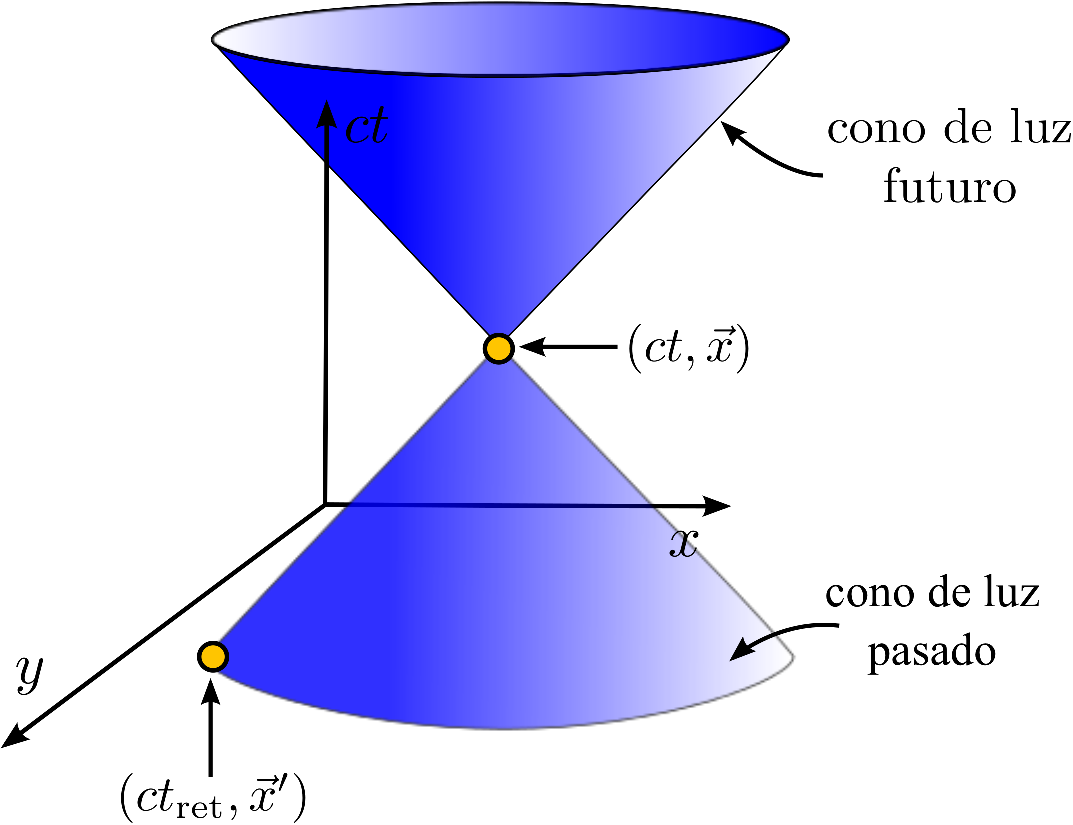
\psfig{file=fig/fig-cono-de-luz-01.pdf,height=5.5cm,angle=0}}
\caption{Cono de luz}
\label{fig:cdl2}
\end{figure}

Otra consecuencia directa es que cualquier \textit{cambio} en la configuraci'on de las fuentes en un punto afectar'a a los campos en otro punto s'olo en tiempos posteriores, luego de un intervalo de tiempo igual al tiempo de vuelo de una se\~nal luminosa que los conecte. En otras palabras: \textit{los cambios de los campos producidos por cambios de las fuentes se propagan con rapidez $c=1/\sqrt{\varepsilon\mu}$}. Equivalentemente, el valor de las fuentes en un determinado evento contribuye a los valores de los campos s'olo en eventos situados sobre el \textit{cono de luz futuro} del evento fuente.

\section{Ecuaciones de Jefimenko}
A partir de las expresiones para los potenciales retardados en el gauge de Lorenz, es decir las ecuaciones \eqref{potret}, podemos calcular los campos el'ectrico y magn'etico producidos por una distribuci'on (arbitraria, pero compacta) de cargas y corrientes:
\begin{equation}
\vec{E}(\vec{x},t)=\frac{1}{4\pi\varepsilon}\int_V \left[  \frac{\rho(\vec{x}',t_{\rm ret})(\vec{x}-\vec{x}')}{\vert \vec{x}-\vec{x}' \vert^3} + \frac{1}{c}\frac{ \dot\rho(\vec{x}',t_{\rm ret})(\vec{x}-\vec{x}')}{\vert\vec{x}-\vec{x}'\vert^2} -\frac{1}{c^2}\frac{\dot{\vec{J}} (\vec{x}',t_{\rm ret})}{\vert\vec{x}-\vec{x}' \vert} \right] dV',
\end{equation}
\begin{equation}
\vec{B}(\vec{x},t)=\frac{\mu}{4\pi} \int_V\left[
\frac{\vec{J}(\vec{x}',t_{\rm ret})\times(\vec{x}-\vec{x}')}{\vert \vec{x}-\vec{x}'\vert^3}+ \frac{1}{c}\frac{ \dot{\vec{J}}(\vec{x}',t_{\rm ret})\times(\vec{x}-\vec{x}')}{\vert\vec{x}-\vec{x}' \vert^2} \right]dV', \label{b3}
\end{equation}
donde $\dot{f}(\vec{x},t)$ denota la derivada partial respecto a la variable temporal de la que depende la funci'on $f(\vec{x},t)$, es decir $\dot{f}(\vec{x},t):=(\partial_t f)(\vec{x},t)$. Las relaciones anteriores son conocidas como \textbf{ecuaciones de Jefimenko}\footnote{\href{http://en.wikipedia.org/wiki/Jefimenko}{Oleg Jefimenko} (1922-2009): f'isico estadounidense.}. Note que estas expresiones para los campos el'ectrico y magn'etico difieren de aquellas que se encontrar'ian directamente la soluci'on de las ecuaciones inhomog'eneas \eqref{EcOihE} y \eqref{EcOihB}. ?`Puede explicar por qu'e ocurre esto?.


\section{Potenciales de Li'enard-Wiechert}

Se conoce como \textbf{potenciales de Li'enard}\footnote{\href{https://en.wikipedia.org/wiki/Alfred-Marie_Li\%C3\%A9nard}{Alfred Marie Li\'enard} (1869-1958): f'isico franc'es.}\textbf{-Wiechert}\footnote{\href{https://en.wikipedia.org/wiki/Emil_Wiechert}{Johann Emil Wiechert} (1861-1928): (geo)f'isico alem'an.} a los potenciales retardados generados por una \textit{carga puntual} $q$ \textit{que se mueve en forma conocida, pero arbitraria, con trayectoria} $\vec{z}(t)$. Ver figura (\ref{fig:LW}).
\begin{figure}[ht]
\centerline{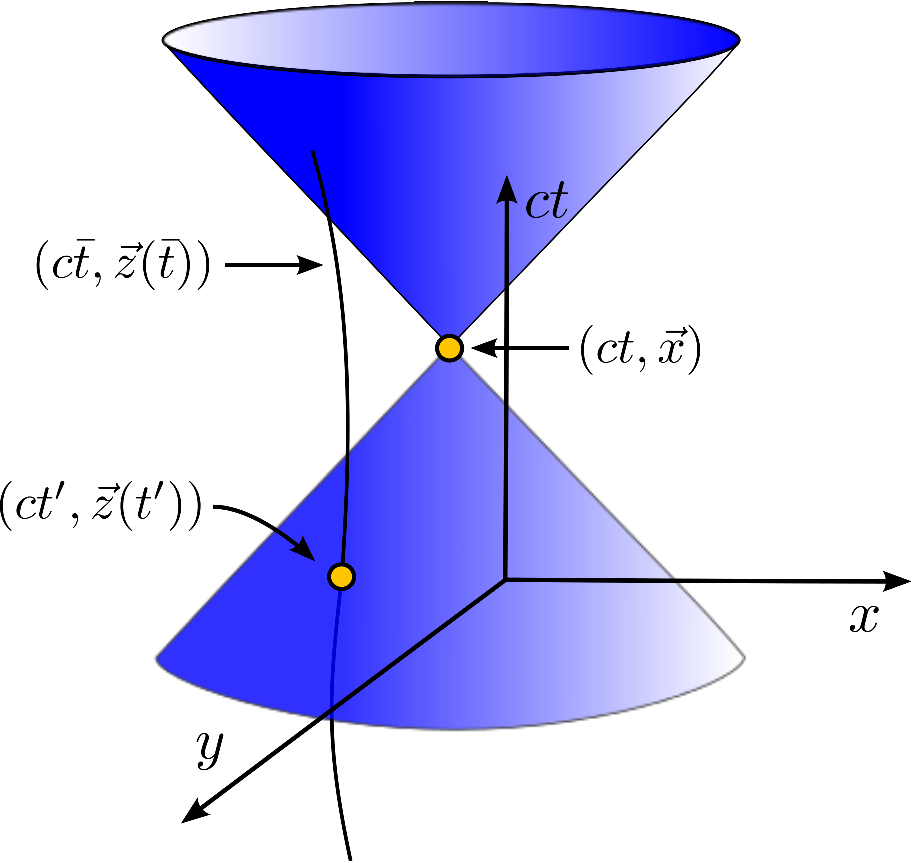
\psfig{file=fig/fig-cono-de-luz-02.pdf,height=5.5cm,angle=0}}
\caption{Trayectoria de una carga puntual y cono de luz asociado al evento $(ct,\vec{x})$.}
\label{fig:LW}
\end{figure}
En este caso, la densidad de carga y de corriente est'an dadas por
\begin{equation}
\rho(\vec{x},t)=q\delta^{(3)}(\vec{x}-\vec{z}(t)), \qquad
\vec{J}(\vec{x},t)=q\vec{v}(t)\delta^{(3)}(\vec{x}-\vec{z}(t)),
\end{equation}
donde $\vec{v}(t)={d\vec{z}}/{dt}$. Por lo tanto, los potenciales retardados (\ref{potret}) se reducen a
\begin{equation}
\phi_{\rm ret}(\vec{x},t)=\frac{q}{4\pi\varepsilon}\int_{V'}
\frac{\delta^{(3)}(\vec{x}'-\vec{z}(t_{\rm ret}))}{|\vec{x}-\vec{x}'|}\,dV', \qquad
\vec{A}_{\rm ret}(\vec{x},t)=\frac{q\mu}{4\pi}\int_{V'}
\frac{\vec{v}(t_{\rm ret})\delta^{(3)}(\vec{x}'-\vec{z}(t_{\rm ret}))}{|\vec{x}-\vec{x}'|}\,dV'  \label{potretq1}
\end{equation}
o, m'as expl'icitamente,
\begin{equation}
\phi_{\rm ret}(\vec{x},t)=\frac{q}{4\pi\varepsilon}\int_{V'}
\frac{\delta^{(3)}(\vec{x}'-\vec{z}(t-|\vec{x}-\vec{x}'|/c))}{|\vec{x}-\vec{x}'|}\,dV', \end{equation}
\begin{equation}
\vec{A}_{\rm ret}(\vec{x},t)=\frac{q\mu}{4\pi}\int_{V'}
\frac{\vec{v}(t-|\vec{x}-\vec{x}'|/c)\,\delta^{(3)}(\vec{x}'-\vec{z}(t-|\vec{x}-\vec{x}'|/c))}{|\vec{x}-\vec{x}'|}\,dV' . \label{potretq2}
\end{equation}
Ambas expresiones son de la forma
\begin{equation}
I(\vec{x},t)=\int_{V'}
f(\vec{x},\vec{x}',t)\,\delta^{(3)}(\vec{x}'-\vec{z}(t-|\vec{x}-\vec{x}'|/c))\,d^3x' . \label{potretqg1}
\end{equation}

Para calcular este tipo de integrales, expresaremos la delta de Dirac 3-dimensional como una integral sobre la variable (temporal) auxiliar $T$:
\begin{equation}
 \delta^{(3)}(\vec{x}'-\vec{z}(t-|\vec{x}-\vec{x}'|/c))=\int_T \delta^{(3)}(\vec{x}'-\vec{z}(T))\,\delta(T-t+|\vec{x}-\vec{x}'|/c)\, dT.
\end{equation}
Con esto,
\begin{equation}
I(\vec{x},t)=\int_{T}\int_{V'}
f(\vec{x},\vec{x}',t)\,\delta^{(3)}(\vec{x}'-\vec{z}(T))\,\delta(T-t+|\vec{x}-\vec{x}'|/c)\,d^3x' \, dT. \label{potretqgm11}
\end{equation}
Expresada de esta forma, es sencillo realizar la integral espacial, puesto que la delta de Dirac 3-dimensional evaluar'a la coordenada $\vec{x}'$ en el punto $\vec{z}(T)$, es decir, en un punto sobre la trayectoria de la carga. As'i, obtenemos
\begin{equation}
I(\vec{x},t)=\int_{T}f(\vec{x},\vec{z}(T),t)\,\delta(T-t+|\vec{x}-\vec{z}(T)|/c)\, dT. \label{potretqgm12}
\end{equation}
El argumento de la delta de Dirac es una funci'on no trivial $g$ de la variable auxiliar $T$. Denotamos
\begin{equation}
 g(T):=T-t+\frac{1}{c}|\vec{x}-\vec{z}(T)|,
\end{equation}
de modo que
\begin{eqnarray}
I(\vec{x},t)&=&\int_{T}f(\vec{x},\vec{z}(T),t)\,\delta(g(T))\, dT \\
&=&\int_{T}f(\vec{x},\vec{z}(T),t)\frac{\delta(T-t')}{|g'(t')|}\, dT \\
&=&\frac{f(\vec{x},\vec{z}(t'),t)}{|g'(t')|}, \label{Ir}
\end{eqnarray}
donde $g'$ es la funci'on derivada de $g$ y $t'$ es la soluci'on de la ecuaci'on $g(t')=0$, es decir, de
\begin{equation}
 t'=t-\frac{1}{c}|\vec{x}-\vec{z}(t')|. \label{t'}
\end{equation}
Esta relaci'on define una ecuaci'on algebraica para $t'$ cuya soluci'on define, \textit{conocida la trayectoria de la carga}, un tiempo retardado $t'=t'(\vec{x},t)$. Adem'as, usando la regla de la cadena, encontramos
\begin{equation}
 g'(t')=1-\frac{1}{c}\frac{\vec{v}(t')\cdot\left(\vec{x}-\vec{z}'(t')\right)}{\left|\vec{x}-\vec{z}(t')\right|}=1-\vec{\beta}(t')\cdot\hat{n}(t')>0 \label{gp},
\end{equation}
para $|\vec\beta|<1$, con $\vec\beta:=\vec{v}/c$. Por ahora, supondremos que siempre la velocidad de la part'icula es menor que la velocidad de la luz en el medio. Entonces, reemplazando (\ref{gp}) en (\ref{Ir}), se encuentra que
\begin{equation}
 I(\vec{x},t)=\frac{f(\vec{x},\vec{z}(t'),t)}{1-\vec{\beta}(t')\cdot\hat{n}(t')}. \label{Ir2}
\end{equation}
Para el caso del potencial, encontramos as'i que
\begin{equation}
\phi_{\rm ret}(\vec{x},t)=\frac{1}{4\pi\varepsilon}\frac{q}{\left|\vec{x}-\vec{z}(t')\right|}\frac{1}{\left( 1-\vec\beta(t')\cdot\hat{n}(t')\right) }.
 \end{equation}
An'alogamente, en el caso del potencial vectorial, obtenemos
\begin{equation}
\vec{A}_{\rm ret}(\vec{x},t)=\frac{\mu c}{4\pi}\frac{q}{\left|\vec{x}-\vec{z}(t')\right|}
\frac{\vec{\beta}(t')}{\left( 1-\vec\beta(t')\cdot\hat{n}(t')\right) }.
 \end{equation}
 
Debe recordarse que en estas expresiones $t'$ es una funci'on de $\vec{x}$ y $t$, determinada por la soluci'on de (\ref{t'}) para una trayectoria dada. La condici'on (\ref{t'}) implica que el evento donde se quiere determinar el campo, con coordenadas $(ct,\vec{x})$, y el evento sobre la trayectoria de la carga en el tiempo $t'$, con coordenadas $(ct',\vec{z}(t'))$, tienen una \textit{relaci'on tipo luz}, ya que
\begin{equation}
 c^2(t-t')^2-|\vec{x}-\vec{z}(t')|^2=0.
\end{equation}

En otras palabras, el evento con coordenadas $(ct',\vec{z}(t'))$ es la \textit{intersecci'on entre el cono de luz pasado asociado a $(ct,\vec{x})$ y la l'inea de mundo de la carga}. Ver figura \ref{fig:LW}. Los potenciales en un evento $(ct,\vec{x})$ dado dependen entonces s'olo de las propiedades de la carga (posici'on y velocidad) en el evento $(ct',\vec{z}(t'))$.

Usualmente, se simplifica la notaci'on definiendo
\begin{equation}
 \vec{R}:=\vec{x}-\vec{z}(t'), \qquad R:=\left|\vec{x}-\vec{z}(t')\right|, \qquad \hat{n}:=\frac{\vec{R}}{R}, \label{defR}
\end{equation}
y denotando la evaluaci'on de todas las funciones dependientes del tiempo en $t'$ por $f(t'):=\left.f\right|_{\rm ret}$, de modo que
\begin{equation}
\boxed{\phi_{\rm ret}(\vec{x},t)=\frac{1}{4\pi\varepsilon}\left. \frac{q}{ R\left(
1-\vec{\beta}\cdot\hat{n}\right) }\right|_{\rm ret}, } \qquad
\boxed{\vec{A}_{\rm ret}(\vec{x},t)=\frac{\mu c}{4\pi}\left. \frac{q\vec{\beta}}{ R\left(1-\vec{\beta}\cdot\hat{n}\right) }\right|_{\rm ret}.} \label{potretq}
\end{equation}

Note que en este caso los potenciales retardados est'an relacionados por
\begin{equation}
\vec{A}_{\rm ret}(\vec{x},t)=\frac{1}{c}\phi_{\rm ret}(\vec{x},t)\left.\vec{\beta}\right|_{\rm ret}.
\end{equation}


\subsection{Derivaci'on alternativa*}
Podemos integrar (\ref{potretqg1}) cambiando de variable de integraci'on de $\vec{x}'$ a la nueva variable $\vec{y}$, definida por (recu'erdese que, para efectos de la integraci'on, $t$ es un par'ametro y $\vec{z}$ una funci'on conocida)
\begin{equation}
 \vec{y}(\vec{x'}):=\vec{x}'-\vec{z}(t-|\vec{x}-\vec{x}'|/c). \label{txy}
\end{equation}
En t'erminos de $\vec{y}$ la integral (\ref{potretqg1}) adopta la forma
\begin{equation}
I(\vec{x},t)=\int f(\vec{x},\vec{x}'(\vec{y}),t)\delta^{(3)}(\vec{y})
\left|\frac{\partial \vec{x}}{\partial \vec{y}}\right|\,d^3y, \label{potretqg2}
\end{equation}
donde $\left|\frac{\partial \vec{x}'}{\partial \vec{y}}\right|=\left|\frac{\partial \vec{y}}{\partial \vec{x}'}\right|^{-1}$ es el jacobiano de la transformaci'on. A partir de (\ref{txy}) encontramos que
\begin{eqnarray}
\frac{\partial y^i}{\partial x'^j}&=&\delta^i_j-\dot{z}^i(t_{\rm ret})\frac{\partial t_{\rm ret}}{\partial x'^j} \\
&=&\delta^i_j+\frac{1}{c}v^i(t_{\rm ret})\partial'_j|\vec{x}-\vec{x}'|\\
&=&\delta^i_j-\beta^i(t_{\rm ret})\frac{(x^j-x'^j)}{|\vec{x}-\vec{x}'|}\\
&=&\delta^i_j-\beta^i(t_{\rm ret})\hat{n}^j.
\end{eqnarray}
% donde hemos introducido el vector de velocidad adimensionalizado $\vec{\beta}$ y definido el vector unitario $\vec{n}(\vec{x},\vec{x}'):=\frac{(\vec{x}-\vec{x}')}{|\vec{x}-\vec{x}'|}$.
Un c'alculo directo muestra que
\begin{equation}
 \left|\frac{\partial \vec{y}}{\partial \vec{x}'}\right|=1-\vec\beta\cdot\hat{n}.
\end{equation}
Con este resultado, podemos reescribir la integral (\ref{potretqg2}) como
\begin{eqnarray}
I(\vec{x},t)&=&\int f(\vec{x},\vec{x}'(\vec{y}),t)\delta^{(3)}(\vec{y})
\left|\frac{\partial \vec{x}}{\partial \vec{y}}\right|\,d^3y \\
&=&\int \delta^{(3)}(\vec{y})
\frac{f(\vec{x},\vec{x}'(\vec{y}),t)}{1-\vec\beta\cdot\hat{n} }\,d^3y . \label{potretqg3}
\end{eqnarray}
La delta de Dirac impone la evaluaci'on del integrando en el punto correspondiente a $\vec{y}=\vec{0}$. De (\ref{txy}) vemos que esto corresponde a evaluar $\vec{x}'$ en el punto del espacio que satisface
\begin{equation}
 \vec{x}'=\vec{z}(t-|\vec{x}-\vec{x}'|/c),
\end{equation}
para un punto evento $(ct,\vec{x})$ dado. Equivalentemente, en t'erminos del tiempo retardado, $\vec{x}'$ debe ser evaluado en aquel punto sobre la trayectoria de la carga por donde 'esta pas'o en el tiempo retardado $t'$, que satisface
\begin{equation}
 t'=t-\frac{1}{c}|\vec{x}-\vec{z}(t')|.
\end{equation}
% La soluci'on de esta condici'on, dada la trayectoria $\vec{z}$, define $t'=t'(\vec{x},t)$.
% Con todo esto, la integral puede escribirse como
% \begin{equation}
%  I(\vec{x},t)=\frac{f(\vec{x},\vec{z}(t'),t)}{\left(
%1-\vec\beta(t')\cdot\hat{n}(\vec{x},\vec{z}(t')\right) }. \label{potretqg3}
% \end{equation}
Con esto, obtenemos
\begin{equation}
 I(\vec{x},t)=\left.\frac{f(\vec{x},\vec{x}'(\vec{y}),t)}{ 1-\vec\beta\cdot\hat{n} } \right|_{\vec{y}=\vec{0}},
\end{equation}
que es equivalente (\ref{Ir2}).

\subsection{Ejemplo: carga en movimiento con velocidad constante}
Consideremos el caso en que la trayectoria de la part'icula es $\vec{z}(t)=\vec{v}t$, con $\vec{v}=v\hat{x}$.

La condici'on (\ref{t'}), que es equivalente a
\begin{equation}
c(t-t')=\left|\vec{x}-\vec{z}(t')\right|=\sqrt{(x-vt')^2+y^2+z^2},
\end{equation}
tiene como soluci'on retardada, $t'<t$, a
\begin{equation}
t'=\gamma^2\left( t-\frac{vx}{c^2}-\frac{1}{c}\sqrt{(x-vt)^2+
(y^2+z^2)\gamma^{-2}}\right) , \qquad \gamma:=\frac{1}{\sqrt{1-v^2/c^2}}.
\end{equation}
Evaluamos la expresi'on en el denominador de las expresiones en \eqref{potretq}. Luego de algo de 'algebra, obtenemos
\begin{equation}
\left[ R\left(1-\vec{\beta}\cdot\hat{n}\right)\right]_{\rm ret}=\sqrt{(x-vt)^2+  \gamma^{-2}(y^2+z^2)}.
\end{equation}
Con esto, los potenciales adoptan la siguiente forma expl'icita:
\begin{eqnarray}
\phi(\vec{x},t)&=&\frac{1}{4\pi\varepsilon}\frac{q}{\sqrt{(x-vt)^2+ \gamma^{-2}(y^2+z^2)}} ,\\
\vec{A}(\vec{x},t)&=&\frac{\mu c}{4\pi} \frac{q\beta\hat{x}}{\sqrt{(x-vt)^2+
\gamma^{-2}(y^2+z^2)}}.
\end{eqnarray}
Derivando, encontramos las expresiones expl'icitas para los campos el'ectrico y magn'etico:
\begin{eqnarray}
B_x(\vec{x},t)&=&0, \\
B_y(\vec{x},t)&=&-\frac{q\mu}{4\pi}\frac{v\gamma^{-2}z}{\left[ (x-vt)^2+
\gamma^{-2}(y^2+z^2)\right]^{3/2}}, \\
B_z(\vec{x},t)&=&+\frac{q\mu}{4\pi}\frac{v\gamma^{-2}y}{\left[(x-vt)^2+
\gamma^{-2}(y^2+z^2)\right]^{3/2}}.
\end{eqnarray}
\begin{eqnarray}
E_x(\vec{x},t)&=&\frac{q}{4\pi\varepsilon}\frac{\gamma^{-2}\left( x-vt\right) }{\left[ (x-vt)^2+
(y^2+z^2)\gamma^{-2}\right] ^{3/2}}, \\
E_y(\vec{x},t)&=&\frac{q}{4\pi\varepsilon}\frac{\gamma^{-2}y}{\left[ (x-vt)^2+
(y^2+z^2)\gamma^{-2}\right] ^{3/2}},\\
E_z(\vec{x},t)&=&\frac{q}{4\pi\varepsilon}\frac{\gamma^{-2}z }{\left[ (x-vt)^2+
(y^2+z^2)\gamma^{-2}\right]
^{3/2}},
\end{eqnarray}
o, en forma un poco m'as compacta,
\begin{equation}\label{EBqvconst}
\vec{E}(\vec{x},t)=\frac{q}{4\pi\varepsilon}\frac{\gamma^{-2}\left(\vec{x}-\vec{v}t\right)}{\left[(x-vt)^2+ (y^2+z^2)\gamma^{-2}\right] ^{3/2}},  \qquad
\vec{B}(\vec{x},t)=\frac{q\mu}{4\pi}\frac{\gamma^{-2}(\vec{v}\times\vec{x})}{\left[(x-vt)^2+\gamma^{-2}(y^2+z^2)\right]^{3/2}}.
\end{equation}
En la secci'on \ref{secEjEBvc} recobraremos este resultado usando transformaciones de Lorentz. Animaciones de estos campos pueden ser encontrados \href{http://ocw.mit.edu/ans7870/8/8.02T/f04/visualizations/electrostatics/04-MovingChargePosElec/04-MovChrgPosElec_f223_320.html}{aqu\'i} para el campo el'ectrico y \href{http://ocw.mit.edu/ans7870/8/8.02T/f04/visualizations/magnetostatics/01-MovingChargePosMag/01-MovChrgMagPos_f223_320.html}{aqu\'i} para el campo magn'etico \cite{MIT}.


\section{Campo electromagn'etico generado por cargas con movimiento acelerado}
\begin{figure}[ht]
\centerline{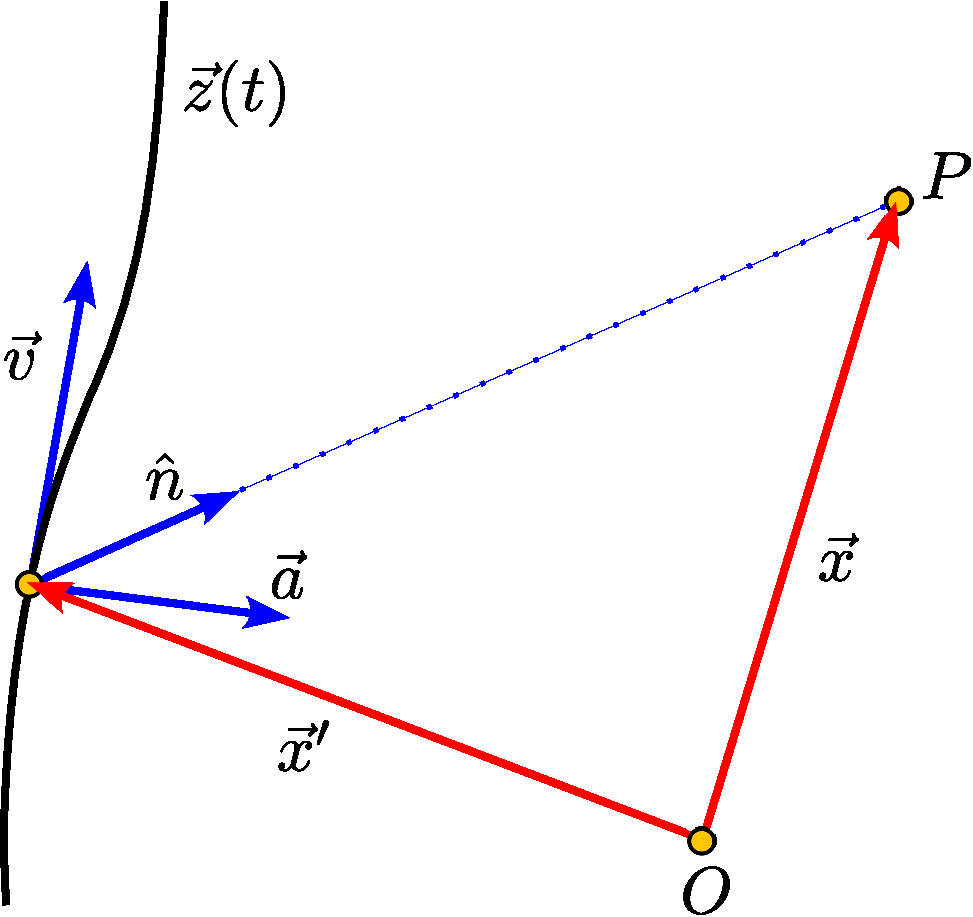
\psfig{file=fig/fig-vectores.pdf,height=5cm,angle=0}} \caption{}
\label{R7}
\end{figure}
Sabemos que los campos el'ectrico y magn'etico est'an dados en t'erminos de derivadas de los potenciales de acuerdo a las expresiones \eqref{defA2} y \eqref{defphi2}. Para evaluar las derivadas involucradas es necesario tener en cuenta que los potenciales retardados dependen de la posici'on $\vec{x}$ y el tiempo $t$ expl'icitamente a trav'es de $\vec{R}=\vec{x}-\vec{z}(t')$ y $\vec{n}$, \textit{pero adem'as impl'icitamente a trav'es del tiempo retardado} $t'=t'(\vec{x},t)$, que es soluci'on de \eqref{t'}.

Tomando en cuenta esta doble dependencia, calculamos:
\begin{eqnarray}
 \partial_i\phi&=&\frac{q}{4\pi\varepsilon}\partial_i\left[\frac{1}{R-\vec{\beta}\cdot\vec{R}}\right] \\
&=&-\frac{q}{4\pi\varepsilon}\frac{1}{(R-\vec{\beta}\cdot\vec{R})^2}\left[\partial_iR-\frac{1}{c}a_j(t')R_j\partial_i t'-\beta_j\partial_iR_j\right].
\end{eqnarray}
Derivando $R^2=R_jR_j$ encontramos que
\begin{equation}
\partial_i R=\hat{n}_j\partial_i R_j. \label{diR}
\end{equation}
Por otro lado, la definici'on (\ref{defR}a) implica que
\begin{equation}
 \partial_i R_j=\partial_i( x_j-z_j(t'))=\delta_{ij}-c\beta_j\partial_i t' . \label{diRj}
\end{equation}
Adem'as, la condici'on (\ref{t'}) permite escribir las derivadas de $t'$ en t'erminos de las derivadas de $R$:
\begin{equation}
 \partial_i t'=\partial_i(t-\frac{1}{c}R)=-\frac{1}{c}\partial_iR. \label{dit'}
\end{equation}
Reemplazando (\ref{diR}) en (\ref{dit'})  y luego usando (\ref{diRj}) obtenemos
\begin{equation}
 \partial_i t'=-\frac{1}{c}\hat{n}_i+(\vec{\beta}\cdot\hat{n})\partial_it', \label{dit'2}
\end{equation}
que nos permite encontrar una expresi'on para $\partial_it'$ en t'erminos de $\hat{n}$ y $\vec{\beta}$:
\begin{equation}
 \boxed{\partial_i t'=-\frac{1}{c}\frac{\hat{n}_i}{1-\vec{\beta}\cdot\hat{n}}.}
\end{equation}
Reemplazando este resultado en (\ref{diRj}) y en (\ref{diR}) obtenemos expresiones similares para las otras derivadas que necesitamos:
\begin{equation}
 \boxed{\partial_i R_j=\delta_{ij}+\frac{\beta_j\hat{n}_i}{1-\vec{\beta}\cdot\hat{n}},}
\end{equation}
\begin{equation}
\boxed{\partial_i R=\frac{\hat{n}_i}{1-\vec{\beta}\cdot\hat{n}}.}
\end{equation}
Con esta informaci'on, podemos expresar el gradiente del potencial escalar como
\begin{equation}
 \partial_i\phi=-\frac{q}{4\pi\varepsilon}\frac{1}{(R-\vec{\beta}\cdot\vec{R})^2} \left[\frac{\hat{n}_i}{1-\vec{\beta}\cdot\hat{n}}+\frac{1}{c^2}\frac{(\vec{a}\cdot\vec{R})\hat{n}_i}{1-\vec{\beta}\cdot\hat{n}} -\beta_i-\frac{\beta^2\hat{n}_i}{1-\vec{\beta}\cdot\hat{n}}\right],
\end{equation}
o, en notaci'on vectorial,
\begin{equation}
 \vec\nabla\phi=-\frac{q}{4\pi\varepsilon}\frac{1}{(R-\vec{\beta}\cdot\vec{R})^2}\left[\frac{\hat{n}}{\gamma^2(1-\vec{\beta}\cdot\hat{n})}+\frac{1}{c^2}\frac{(\vec{a}\cdot\vec{R})\hat{n}}{1-\vec{\beta}\cdot\hat{n}}-\vec\beta\right].
\end{equation}
Similarmente, calculamos la derivada temporal del potencial vectorial:
\begin{eqnarray}
 \partial_t A_i&=&\frac{q\mu c}{4\pi}\partial_t\left[\frac{\beta_i}{R-\vec{\beta}\cdot\vec{R}}\right] \\
&=&\frac{q\mu c}{4\pi}\left[\frac{1}{c}\frac{a_i\partial_tt'}{(R-\vec{\beta}\cdot\vec{R})}-\frac{\beta_i}{(R-\vec{\beta}\cdot\vec{R})^2}\left(\partial_tR-\frac{1}{c}a_j(t')R_j\partial_t t'-\beta_j\partial_tR_j\right)\right] \\
&=&\frac{\mu c}{4\pi}\frac{q}{(R-\vec{\beta}\cdot\vec{R})^2}\left[\frac{1}{c}a_i(R-\vec{\beta}\cdot\vec{R})\partial_tt'-\beta_i\partial_tR+\frac{1}{c}\beta_ia_jR_j\partial_t t'+\beta_i\beta_j\partial_tR_j\right] . \label{dtA}
\end{eqnarray}
Las derivadas del lado derecho de la expresi'on anterior pueden calcularse usando el mismo m'etodo antes usado: Derivando $R^2=R_jR_j$, (\ref{defR}a) y (\ref{t'}) encontramos, respectivamente, que
\begin{equation}
\partial_t R=\hat{n}\cdot\partial_t \vec{R}, \label{dtR}
\end{equation}
\begin{equation}
 \partial_t \vec{R}=\partial_t( \vec{x}-\vec{z}(t'))=-c\vec{\beta}\,\partial_t t', \label{dtRj}
\end{equation}
\begin{equation}
 \partial_t t'=\partial_t(t-\frac{1}{c}R)=1-\frac{1}{c}\partial_tR. \label{dtt'}
\end{equation}
Sustituyendo (\ref{dtR}) en (\ref{dtt'})  y luego usando (\ref{dtRj}) llegamos a
\begin{equation}
 \partial_t t'=1+(\vec{\beta}\cdot\hat{n})\partial_tt',
\end{equation}
de donde podemos despejar $\partial_t t'$, obteniendo
\begin{equation}
 \boxed{\partial_t t'=\frac{1}{1-\vec{\beta}\cdot\hat{n}}.} \label{dtt'2}
\end{equation}
Con esto, (\ref{dtRj}) y (\ref{dtR}) determinan las derivadas faltantes:
\begin{equation}
 \boxed{\partial_t \vec{R}=-\frac{c\vec\beta}{1-\vec{\beta}\cdot\hat{n}},}
\end{equation}
\begin{equation}
\boxed{\partial_t R=-\frac{c(\vec\beta\cdot\hat{n})}{1-\vec{\beta}\cdot\hat{n}}.}
\end{equation}
Sustituci'on en (\ref{dtA}) conduce entonces a
\begin{eqnarray}
 \partial_t \vec{A}
&=&\frac{\mu c}{4\pi}\frac{q}{(R-\vec{\beta}\cdot\vec{R})^2}\left[\frac{1}{c}\vec{a}R+\frac{1}{c}
\frac{\vec{\beta}(\vec{a}\cdot\vec{R})}{(1-\vec{\beta}\cdot\hat{n})}+\frac{c\vec\beta}{1-\vec{\beta}\cdot\hat{n}}(\vec{\beta}\cdot\hat{n}-\beta^2)\right] \\
&=&\frac{\mu c}{4\pi}\frac{q}{(R-\vec{\beta}\cdot\vec{R})^2}\left[\frac{1}{c}\vec{a}R+\frac{1}{c}
\frac{\vec{\beta}(\vec{a}\cdot\vec{R})}{(1-\vec{\beta}\cdot\hat{n})}-c\vec\beta+\frac{c\vec\beta}{\gamma^2(1-\vec{\beta}\cdot\hat{n})}\right] \\
&=&\frac{1}{4\pi\varepsilon}\frac{q}{(R-\vec{\beta}\cdot\vec{R})^2}\left[\frac{1}{c^2}\vec{a}R+\frac{1}{c^2}\frac{\vec{\beta}(\vec{a}\cdot\vec{R})}{(1-\vec{\beta}\cdot\hat{n})}-\vec\beta+\frac{\vec\beta}{\gamma^2(1-\vec{\beta}\cdot\hat{n})}\right] .
\end{eqnarray}
Tenemos ahora los ingredientes necesarios para calcular el campo el'ectrico:
\begin{eqnarray}
4\pi\varepsilon\vec{E}&=&\frac{q}{(R-\vec{\beta}\cdot\vec{R})^2}\left[\frac{\hat{n}}{\gamma^2(1-\vec{\beta}\cdot\hat{n})}+\frac{1}{c^2}\frac{(\vec{a}\cdot\vec{R})\hat{n}}{(1-\vec{\beta}\cdot\hat{n})}-\vec\beta-\frac{1}{c^2}\vec{a}R-\frac{1}{c^2}\frac{\vec{\beta}(\vec{a}\cdot\vec{R})}{(1-\vec{\beta}\cdot\hat{n})}+\vec\beta-\frac{\vec\beta}{\gamma^2(1-\vec{\beta}\cdot\hat{n})}\right] \nonumber \\
&=&\frac{q}{(R-\vec{\beta}\cdot\vec{R})^2}\left[\frac{\hat{n}-\vec\beta}{\gamma^2(1-\vec{\beta}\cdot\hat{n})}+\frac{1}{c^2}\frac{(\vec{a}\cdot\vec{R})\hat{n}}{(1-\vec{\beta}\cdot\hat{n})}-\frac{1}{c^2}\vec{a}R-\frac{1}{c^2}\frac{\vec{\beta}(\vec{a}\cdot\vec{R})}{(1-\vec{\beta}\cdot\hat{n})}\right] \\
&=&\frac{q(\hat{n}-\vec\beta)}{\gamma^2R^2(1-\vec{\beta}\cdot\hat{n})^3}+\frac{q}{c^2(R-\vec{\beta}\cdot\vec{R})^2}\left[\frac{(\vec{a}\cdot\vec{R})\hat{n}}{(1-\vec{\beta}\cdot\hat{n})}-\vec{a}R-\frac{\vec{\beta}(\vec{a}\cdot\vec{R})}{(1-\vec{\beta}\cdot\hat{n})}\right] \\
&=&\frac{q(\hat{n}-\vec\beta)}{\gamma^2R^2(1-\vec{\beta}\cdot\hat{n})^3}+\frac{q}{c^2R^2(1-\vec{\beta}\cdot\hat{n})^3}\left[(\vec{a}\cdot\vec{R})\hat{n}-\vec{a}R+\vec{a}\vec{\beta}\cdot\vec{R}-\vec{\beta}(\vec{a}\cdot\vec{R})\right] \\
&=&\frac{q(\hat{n}-\vec\beta)}{\gamma^2R^2(1-\vec{\beta}\cdot\hat{n})^3}+\frac{q}{c^2R(1-\vec{\beta}\cdot\hat{n})^3}\left[(\vec{a}\cdot\hat{n})(\hat{n}-\vec{\beta})-\vec{a}+\vec{a}\vec{\beta}\cdot\hat{n}\right] .
\end{eqnarray}
Usando la identidad
\begin{equation}
(\vec{a}\cdot\hat{n})(\hat{n}-\vec{\beta})-\vec{a}+\vec{a}\vec{\beta}\cdot\hat{n}\equiv (\vec{a}\cdot\hat{n})(\hat{n}-\vec{\beta})-\vec{a} (1-\hat{n}\cdot\vec\beta)\equiv \hat{n}\times\left[ \left( \hat{n}-\vec{\beta}\right)
\times{\vec{a}}\right],
\end{equation}
encontramos finalmente que\textit{ el campo el'ectrico generado por una carga $q$ en movimiento arbitrario} es de la forma
\begin{equation}\marginnote{campo $\vec{E}$ carga $q$}
\boxed{\vec{E}(\vec{x},t)=\vec{E}_{(1)}+\vec{E}_{(2)}=\frac{q}{4\pi\varepsilon}\left.\frac{\left(
\hat{n}-\vec{\beta}\right)
}{\gamma^2R^2\left(1-\vec{\beta}\cdot\hat{n}\right)^3}\right|_{\rm ret}+
\frac{q\mu}{4\pi}\left.\frac{\hat{n}\times\left[ \left( \hat{n}-\vec{\beta}\right)
\times{\vec{a}}\right] }{R\left( 1-\vec{\beta}\cdot\hat{n}\right)
^3}\right|_{\rm ret} .} \label{Egen}
\end{equation}
El campo magn'etico puede calcularse de forma similar, encontr'andose que \textit{puede expresarse completamente en t'erminos del campo el'ectrico}:
\begin{equation}\marginnote{campo $\vec{B}$ carga $q$}
\boxed{\vec{B}(\vec{x},t)=\frac{1}{c}\left. \hat{n}\right|_{\rm
ret}\times\vec{E}(\vec{x},t) .}
\end{equation}
Este resultado muestra, por lo tanto, que \textit{el campo magn'etico producido por una carga puntual es, en cada punto del espacio, perpendicular al campo el'ectrico y al vector que une la posici'on \underline{retardada} de la carga con el punto de observaci'on}.

Note que para distancias $r$ muy grandes (comparadas con las dimensiones de la
regi'on donde se encuentran las fuentes, que consideramos una regi'on compacta) $R\approx r$ y entonces
$\vec{E}_{(1)}\propto r^{-2}$ mientras que $\vec{E}_{(2)}\propto
r^{-1}$.


\section{Potencia Radiada}

Consideramos un sistema de cargas y corrientes confinado a una regi'on compacta del espacio (por ejemplo, la carga puntual analizada en la secci'on anterior). El campo electromagn'etico que este sistema produce tiene asociado un vector de flujo de energ'ia, el vector de Poynting. La potencia (es decir, la energ'ia por unidad de tiempo) total transferida por el campo electromagn'etico generado por las cargas y corrientes, a trav'es de una superficie que encierra completamente al sistema, y elegida por conveniencia como una esfera de radio $r$, es dada por
\begin{equation}
P(r,t)=\int_S \vec{S}\cdot d\vec{S}=\frac{1}{\mu}\int_S \left[ \left(
\vec{E}\times\vec{B}\right) \cdot \hat{r}\right] \,r^2d\Omega.
\end{equation}

Llamamos \textbf{potencia radiada} a la energ'ia que es transportada \textit{muy lejos} de las fuentes, es decir $r\gg L$ donde $L$ es el tama\~no (lineal) caracter'istico del sistema, y que \textit{aproximamos} por el l'imite en que $r\rightarrow\infty$. En este l'imite, ubicando el centro de la esfera en un punto representativo de la distribuci'on de cargas y corrientes, podemos aproximar $\hat{n}\approx\hat{r}$ y $R\approx r$ de modo que,
\begin{equation}
P_{\rm rad} (t)=\lim_{r\rightarrow\infty}\frac{1}{\mu}\int_S \left[ \left(
\vec{E}\times\vec{B}\right) \cdot \hat{n}\right] \,r^2 d\Omega.
\end{equation}

Tomando en cuenta la dependencia de $\vec{E}_{(1)}$ y $\vec{E}_{(2)}$ con $r$
podemos ver que s'olo los t'erminos provenientes de $\vec{E}_{(2)}$
contribuir'an a $P_{\rm rad}(t)$ en el l'imite $r\rightarrow\infty$, es decir,
\begin{equation}\label{Pinf1}
P_{\rm rad}(t)=\lim_{r\rightarrow\infty}\int_S \vec{S}_{(2)}\cdot
d\vec{S}=\frac{1}{\mu}\lim_{r\rightarrow\infty}\int_S \left[ \left(
\vec{E}_{(2)}\times\vec{B}_{(2)}\right) \cdot \hat{n}\right] \,r^2 d\Omega.
\end{equation}
En otras palabras, el sistema rad'ia energ'ia (``al infinito'') \textit{s'olo si la
carga acelera}. Por esto, $\vec{E}_{(2)}$ recibe el nombre de \textbf{campo de
radiaci'on} o \textbf{campo lejano}, mientras que $\vec{E}_{(1)}$ es llamado
\textbf{campo cercano}.

Calculamos ahora la parte del vector de Poynting que contribuir'a a la energ'ia
radiada fuera del sistema (al infinito):
\begin{equation}
 \vec{S}_{(2)}:=\frac{1}{\mu}\, \vec{E}_{(2)}\times\vec{B}_{(2)},
\end{equation}
con
\begin{equation}
\vec{B}_{(2)}= \frac{1}{c}\hat{n}\times\vec{E}_{(2)}.
\end{equation}
Con estos ingredientes encontramos que
\begin{eqnarray}
 \vec{S}_{(2)}&=&\frac{1}{\mu c}\, \vec{E}_{(2)}\times\left(
\hat{n}\times\vec{E}_{(2)}\right) \\
 &=& \frac{1}{\mu c}\left[ \left|\vec{E}_{(2)}\right|^2 \hat{n}-\left(
\vec{E}_{(2)}\cdot\hat{n}\right)  \vec{E}_{(2)}\right].
\end{eqnarray}
Sin embargo, de (\ref{Egen}) vemos que $\vec{E}_{(2)}$ es normal a $\hat{n}$ de
modo que lo anterior se reduce a
\begin{equation}\label{S2E}
 \boxed{\vec{S}_{(2)}= \frac{1}{\mu c} \left|\vec{E}_{(2)}\right|^2 \hat{n},}
\end{equation}
y por lo tanto
\begin{equation}
 \boxed{P_{\rm rad} (t)=\frac{q^2\mu}{16\pi^2c}\lim_{r\rightarrow\infty}\int_\Omega
\left|\left.\frac{\hat{n}\times\left[ \left( \hat{n}-\vec{\beta}\right)
\times{\vec{a}}\right] }{\left( 1-\vec{\beta}\cdot\hat{n}\right)
^3}\right|_{\rm ret}\right|^2 d\Omega.}
\end{equation}

Definimos la potencia radiada \textit{por unidad de 'angulo s'olido}
por
\begin{equation}
 \boxed{\frac{dP_{\rm rad}}{d\Omega}(\hat{n},t):=\frac{q^2\mu}{16\pi^2c}\lim_{r\rightarrow\infty} \left|\left.
\frac{\hat{n}\times\left[ \left( \hat{n}-\vec{\beta}\right)
\times{\vec{a}}\right] }{\left( 1-\vec{\beta}\cdot\hat{n}\right)
^3}\right|_{\rm ret}\right|^2 ,} \label{dPdO}
\end{equation}
de modo que
\begin{equation}
 \boxed{P_{\rm rad}(t)=\int_\Omega \frac{dP_{\rm rad}}{d\Omega}\,d\Omega.}
\end{equation}


\section{F'ormula de Larmor (no-relativista)}\label{sec:Larmor-norel}

Si $v\ll c$, es decir $\beta\ll1$, entonces el campo el'ectrico
(\ref{Egen}) y la distribuci'on de potencia radiada (\ref{dPdO}) pueden
aproximarse por:
\begin{equation}
\vec{E}(\vec{x},t)=\frac{q\mu}{4\pi}\left.\frac{\hat{n}}{R^2}\right|_{\rm ret}+\left.
\frac{q\mu}{4\pi c^2}\frac{\hat{n}\times(\hat{n}\times{\vec{a}})}{R}\right|_{\rm
ret} +O(\beta),
\end{equation}
\begin{equation}
\frac{dP}{d\Omega}=\frac{q^2\mu}{16\pi^2c}\lim_{r\rightarrow\infty}
\left|\hat{n}\times\left[
\hat{n}\times{\vec{a}}\right]\right|^2_{\rm ret}  +O(\beta).
\end{equation}
Aqu'i $|_{\rm ret}$ denota evaluaci'on de las cantidades en el tiempo retardado, que muy lejos de la fuente adopta la forma $t'=t-r/c$.
Introduciendo el 'angulo $\theta$ entre la aceleraci'on $\vec{a}$ y el vector
normal $\hat{n}$, podemos escribir
$\left|\hat{n}\times\left[\hat{n}\times{\vec{a}}\right]\right|^2=\vec{a}^2\sen^2\theta$ y entonces
\begin{equation}
\frac{dP}{d\Omega}(t)=\frac{q^2\mu}{16\pi^2 c}\left[ \vec{a}^2\sen^2\theta\right]_{\rm
ret} .\label{Lardif}
\end{equation}
 Note que la dependencia $\sen^2\theta$ de ${dP}/{d\Omega}$ implica que \textbf{la
energ'ia radiada se dirige mayoritariamente en la direcci'on normal a la
aceleraci'on}. Adem'as, como $\vec{E}_{(2)}\propto
\hat{n}\times(\hat{n}\times{\vec{a}})$ entonces el campo el'ectrico de
radiaci'on  es normal a $\hat{n}$ y est'a contenido en el plano definido por
$\vec{a}$ y $\hat{n}$. Ver figura \ref{fig:natheta}.
 Decimos entonces que el campo de radiaci'on est'a
\textit{polarizado} en el plano definido por $\vec{a}$ y $\hat{n}$ y es normal a
$\hat{n}$. Si $\vec{a}$ es constante, la radiaci'on emitida en una direcci'on $\hat{n}$ dada tiene polarizaci'on 100\% lineal.
\begin{figure}[!h]
\centerline{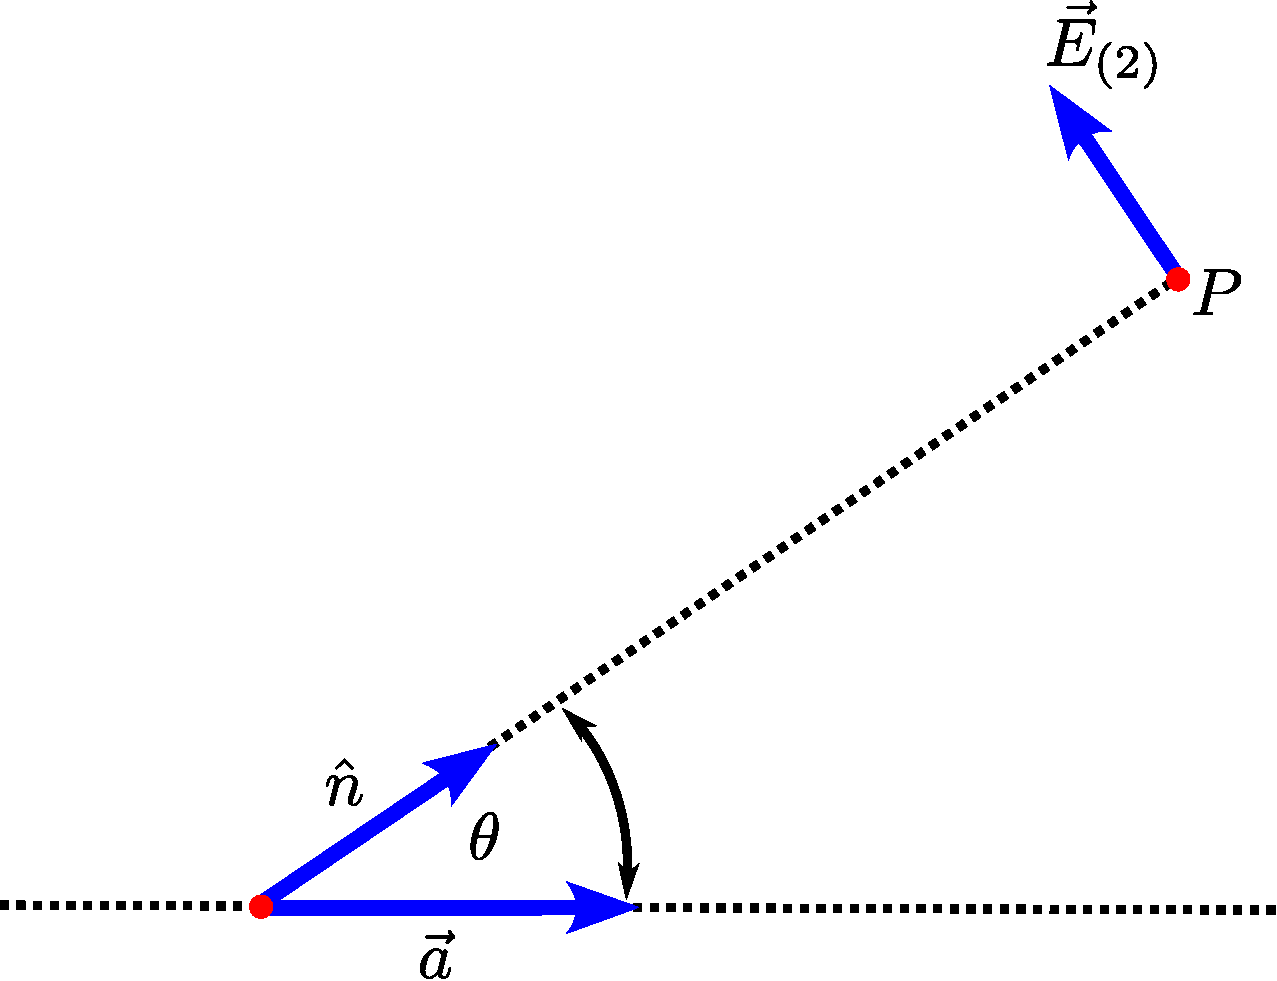
\psfig{file=fig/fig-a-n-Erad.pdf,height=5cm,angle=0}}
\caption{Direcciones de la aceleraci'on $\vec{a}$, vector unitario $\hat{n}$ y campo el'ectrico $\vec{E}_{(2)}$.}
\label{fig:natheta}
\end{figure}
En un \textit{gr'afico de distribuci'on de potencia} (donde se usan coordenadas polares
en las que el radio es identificado con ${dP}/{d\Omega}$, que es funci'on
del 'angulo $\theta$) encontramos una distribuci'on como muestra la figura
\ref{lobulo01}. Vemos entonces que en el l'imite no-relativista la mayor
cantidad de la energ'ia es radiada en direcci'on normal a la aceleraci'on de la
carga.

\begin{figure}[!h]
\centerline{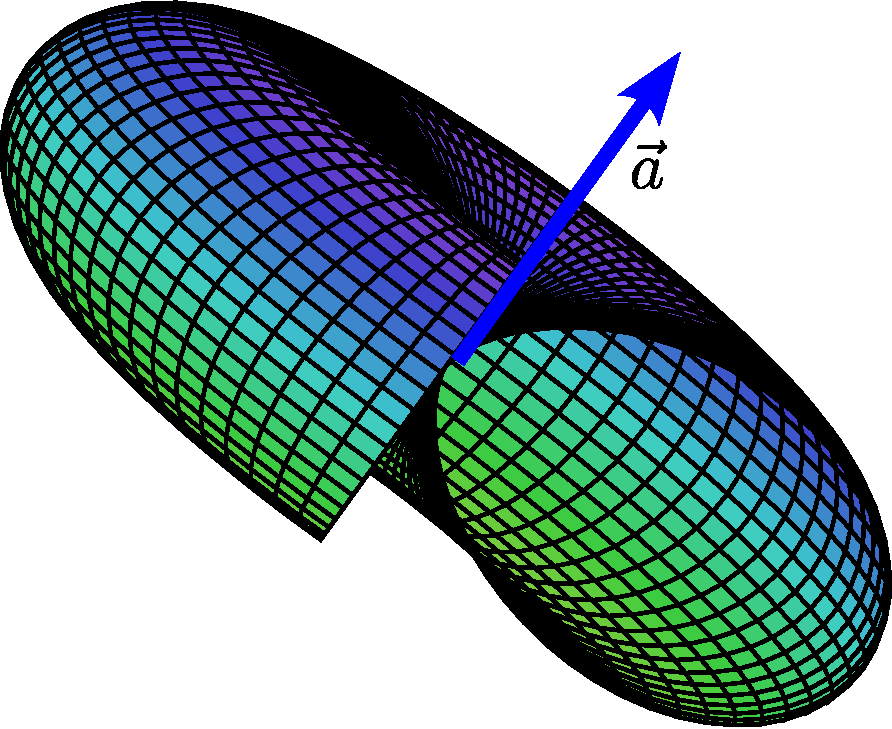
\includegraphics[height=6cm]{fig/fig-Larmor.pdf}\hfill
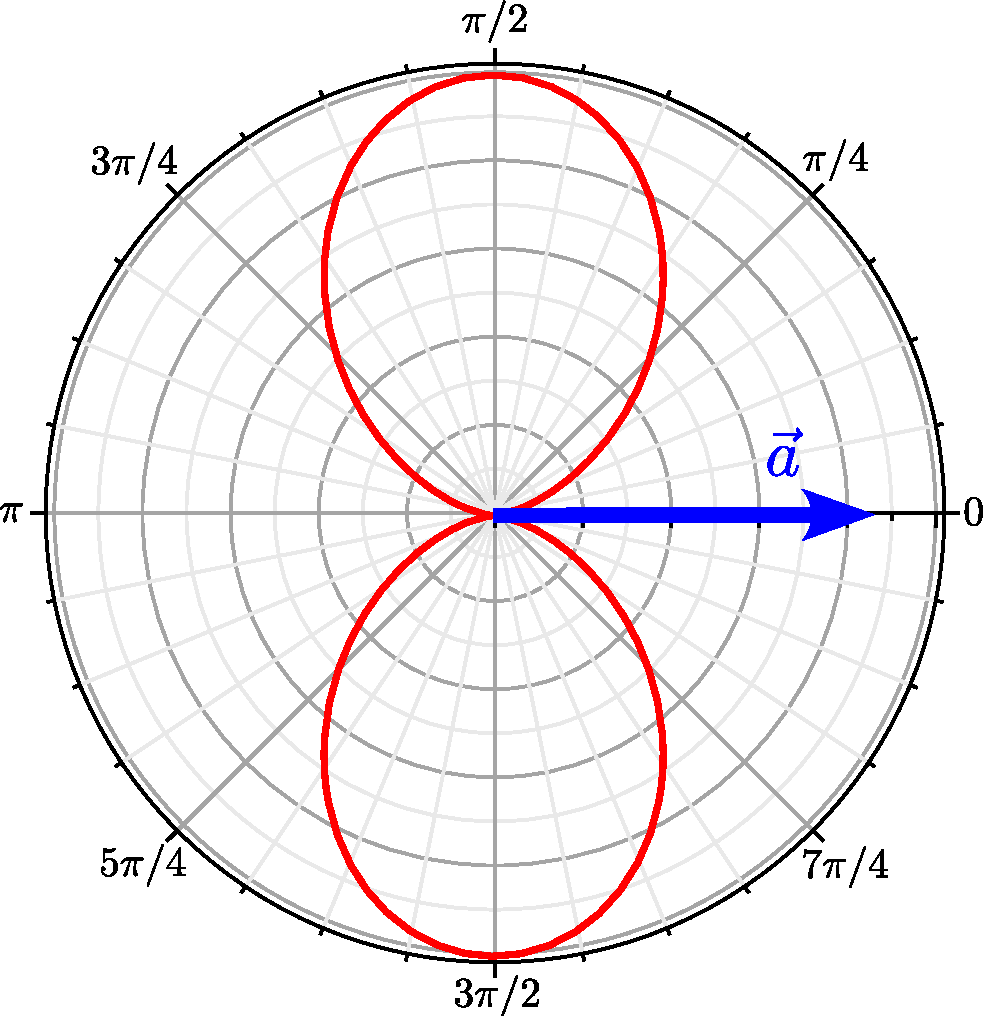
\includegraphics[height=6cm]{fig/fig-Larmor-02.pdf}}
\caption{Distribuci'on de potencia para una carga no-relativista en movimiento
acelerado. C'odigos Python \href{https://github.com/gfrubi/electrodinamica/blob/master/figuras-editables/fig-Larmor-3D.py}{aqu\'i} y \href{https://github.com/gfrubi/electrodinamica/blob/master/figuras-editables/fig-Larmor.py}{aqu\'i}.}
\label{lobulo01}
\end{figure}
La \textit{potencia total emitida} por la carga es entonces
\begin{eqnarray}
P(t)  & =&\int_{\Omega}\frac{dP}{d\Omega}(t)\,d\Omega\\
& =&\frac{q^2\mu}{16\pi^2c}\int_{\Omega} [\vec{a}^2\sen^2\theta]_{\rm ret}\,d\Omega\\
& =&\frac{q^2\mu}{16\pi^2c}\int_0^{\pi}\int_0^{2\pi}\vec{a}^2_{\rm ret}
\sen^2\theta\sen\theta\,d\theta d\varphi \\
& =&\frac{q^2\mu}{16\pi^2c}\,\vec{a}^2_{\rm ret}\, \frac{4}{3}\,2\pi \\
& =&\frac{q^2\mu}{6\pi c}\,\vec{a}^2_{\rm ret}.
\end{eqnarray}
Este resultado es conocido como \emph{f'ormula de Larmor}\footnote{Joseph Larmor (1857-1942): f'isico y matem'atico irland'es. Ver \url{http://es.wikipedia.org/wiki/Joseph_Larmor}.}.
%\begin{equation}
%\boxed{P=\frac{2q^2}{3c^3}\,\vec{a}^2.}\label{R-larmor}
%\end{equation}
\begin{equation}\marginnote{F'ormula de Larmor}
\boxed{P(t)=\frac{q^2\mu}{6\pi c}\,\vec{a}^2_{\rm ret}.}\label{R-larmor}
\end{equation}

Este importante resultado implica, en particular, que cargas de igual magnitud, pero masas distintas sometidas a la acci'on de una misma fuerza (o fuerzas de igual magnitud) rad'ian con potencias distintas si sus masas son distintas. Por ejemplo, \textit{en un sistema formado por protones y electrones, acelerados bajo la acci'on de un mismo campo el'ectrico externo, ser'an los electrones quienes m'as energ'ia radiar'an} puesto que, si bien sus cargas son iguales en m'odulo, la masa de los electrones es mucho menor que la de los protones ($m_{\rm p}\approx 1836\,m_{\rm e}$, ver ap'endice \ref{app:constantes}. Por lo tanto, $P_{\rm e}\approx 3\times 10^6\, P_{\rm p}$). Como consecuencia, en \textit{primera aproximaci'on, son los electrones los principales responsables de la radiaci'on emitida por un sistema}.

%\subsubsection{Ejemplo: Movimiento circular}

\section{Distribuci'on de potencia (correcci'on relativista)}
La energ'ia radiada (muy lejos de la regi'on donde se mueve la carga) es dada por 
\begin{equation}
 E=\int_t\oint_\Omega \frac{dP}{d\Omega}\,d\Omega\,dt=\frac{q^2\mu}{16\pi^2 c}\oint_\Omega\int_t\left.\frac{\left|\hat{n}\times
\left[ \left( \hat{n}-\vec{\beta}\right)\times{\vec{a}}\right]\right|^2}{\left(
1-\hat{n}\cdot\vec{\beta}\right) ^{6}}\right|_{\rm ret}\,dt\,d\Omega .
\end{equation}
Considere el caso particular en que \textit{la carga acelera s'olo en un cierto intervalo de tiempo}, por ejemplo, $\vec{a}(t)\neq\vec{0}$ s'olo entre $t=T_1$ y $t=T_2$. La radiaci'on emitida es entonces causada por la aceleraci'on de la carga en ese periodo de tiempo. Sin embargo, debido a que el integrando est'a evaluado en el tiempo retardado $t'(\vec{x},t)$, el intervalo de tiempo en que se realiza la integraci'on (\ref{Ecasi}) para calcular la energ'ia radiada  (``muy lejos'') difiere del intervalo de tiempo en que la carga aceler'o. 'Esta es una consecuencia de la velocidad finita ($c$) de propagaci'on de las se\~nales electromagn'eticas. En el ejemplo particular analizado, la contribuci'on a la integral s'olo ser'a no nula en un intervalo de tiempo entre $t=t_1$ y $t=t_2$, de modo que
\begin{equation}
 E=\frac{q^2\mu}{16\pi^2 c}\oint_\Omega\int_{t_1}^{t_2}\left.\frac{\left|\hat{n}\times
\left[ \left( \hat{n}-\vec{\beta}\right)\times{\vec{a}}\right]\right|^2}{\left(
1-\hat{n}\cdot\vec{\beta}\right) ^{6}}\right|_{\rm ret}\,dt\,d\Omega , \label{Ecasi}
\end{equation}
y donde los valores $t_1$ y $t_2$ est'an relacionados con $T_1$ y $T_2$ por medio de
\begin{eqnarray}
T_1=t'(\vec{x},t_1)=t_1-\frac{1}{c}|\vec{x}-\vec{z}(T_1)|
\approx t_1-\frac{r}{c}, \\
T_2=t'(\vec{x},t_2)=t_2-\frac{1}{c}|\vec{x}-\vec{z}(T_2)|
\approx t_2-\frac{r}{c},
\end{eqnarray}
es decir, que $T_1$ y $T_2$ son los tiempos retardados asociados a los tiempos $t_1$ y $t_2$. Aqu'i hemos considerado que $r=|\vec{x}|\gg |\vec{z}(t)|$. Ver figura \ref{fig:tiempos}.
\begin{figure}[H]
\centerline{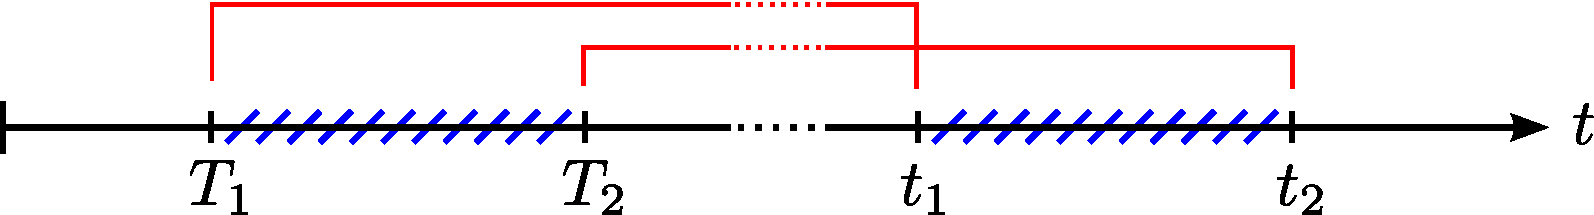
\psfig{file=fig/fig-tiempos.pdf,height=1.5cm,angle=0}}
\caption{Tiempos retardados y tiempos de observaci'on.}
\label{fig:tiempos}
\end{figure}

En resumen, si bien la carga acelera s'olo en el intervalo de tiempo $[T_1,T_2]$, la integral \eqref{Ecasi} para la energ'ia radiada se extiende sobre un intervalo de tiempo diferente (y posterior) $[t_1,t_2]$. En la mayor'ia de las situaciones es m'as conveniente calcular la energ'ia radiada de modo que se integre \textit{directamente en el intervalo de tiempo correspondiente al periodo en que la carga acelera}. Esto equivale a realizar, \textit{para un valor de $\vec{x}'$ fijo dentro de la integral sobre el 'angulo s'olido en \eqref{Ecasi}},  un cambio de variable de $t$ a $t'$, es decir, a escribir
\begin{equation}
 E=\frac{q^2\mu}{16\pi^2 c}\oint_\Omega\int_{T_1}^{T_2}\left.\frac{\left|\hat{n}\times
\left[ \left( \hat{n}-\vec{\beta}\right)\times{\vec{a}}\right]\right|^2}{\left(
1-\hat{n}\cdot\vec{\beta}\right) ^{6}}\right|_{t'}\left(\frac{dt}{dt'}\right)\,dt'd\Omega .\label{Edt'}
\end{equation}
En el cambio de variable anterior las coordenadas espaciales no son variadas, de modo que
\begin{equation}
\frac{dt}{dt'}=\left[\left(\frac{\partial t'}{\partial t}\right)_{\vec{x}=\text{cte.}}\right]^{-1}
=\left[\partial_t t'\right]^{-1}=1-\hat{n}\cdot\vec{\beta}. \label{dtdt'}
\end{equation}
En la 'ultima igualdad hemos usado nuestro resultado (\ref{dtt'2}). Note que esto implica que $dt<dt'$ \textit{si la velocidad de la carga est'a dirigida en la misma direcci'on que el vector} $\vec{n}$ (que apunta desde la carga hasta el punto lejano de observaci'on) y $dt>dt'$ \textit{en caso contrario}. Esta diferencia de intervalos de tiempo corresponde al simple efecto cinem'atico en virtud del cual  la duraci'on de una se\~nal emitida por una fuente luminosa en movimiento es percibida como menor si la fuente se mueve hacia el receptor, y viceversa (efecto Doppler).

Reemplazando (\ref{dtdt'}) en (\ref{Edt'}) obtenemos
\begin{equation}
 E=\frac{q^2\mu}{16\pi^2 c}\oint_\Omega\int_{T_1}^{T_2}\left.\frac{\left|\hat{n}\times\left[ \left( \hat{n}-\vec{\beta}\right)\times{\vec{a}}\right]\right|^2}{\left(1-\hat{n}\cdot\vec{\beta}\right)^5}\right|_{t'}\,dt'd\Omega .\label{Edt'2}
\end{equation}

Ahora \textit{el integrando est'a evaluado en el mismo tiempo usado para la integraci'on}, y por lo tanto s'olo contribuye integrar sobre el intervalo de tiempo en el cual la carga acelera. Puede decirse que la integral (\ref{Edt'2}) permite calcular la energ'ia que \textit{ser'a irradiada} por la carga debido a su movimiento (aceleraci'on) en el intervalo $[T_1,T_2]$.

Podemos consecuentemente definir una correspondiente potencia irradiada por unidad de 'angulo s'olido:
\begin{equation}
\boxed{\frac{dP'}{d\Omega}(t):=\frac{q^2\mu}{16\pi^2 c}\frac{\left|\hat{n}\times
\left[ \left( \hat{n}-\vec{\beta}\right)\times{\vec{a}}\right]\right|^2}{\left(
1-\hat{n}\cdot\vec{\beta}\right) ^{5}},} \label{dP'}
\end{equation}
de modo que
\begin{equation}
 \boxed{E=\int_\Omega\int_{T_1}^{T_2}\frac{dP'}{d\Omega}(t)\,dt\,d\Omega}
\end{equation}
es la energ'ia (\textit{que ser'a}) radiada por la carga, debido a su movimiento entre los tiempos $T_1$ y $T_2$ (es decir, con posici'on inicial $\vec{z}(T_1)$ y final $\vec{z}(T_2)$, etc).

Resumiendo: la potencia (por unidad de 'angulo s'olido) (\ref{dP'}) se diferencia de (\ref{dPdO}) en que la 'ultima es la energ'ia radiada (por unidad de 'angulo s'olido) \textit{por unidad de tiempo transcurrido en los puntos (muy lejanos) de observaci'on}, mientras que (\ref{dP'}) es la energ'ia (que ser'a) radiada (por unidad de 'angulo s'olido) \textit{por unidad de tiempo transcurrido en el movimiento de la carga}. Si bien la energ'ia total radiada dada por las expresiones \eqref{Ecasi} y \eqref{dP'} es la misma, en la mayor'ia de las aplicaciones\footnote{...donde las velocidades de las cargas son relativistas, de otro modo la diferencia es insignificante.} es m'as conveniente describir la distribuci'on de potencia radiada usando \eqref{dP'}.

\subsubsection{Ejemplo: Movimiento unidimensional}
\begin{figure}[!h]
\centerline{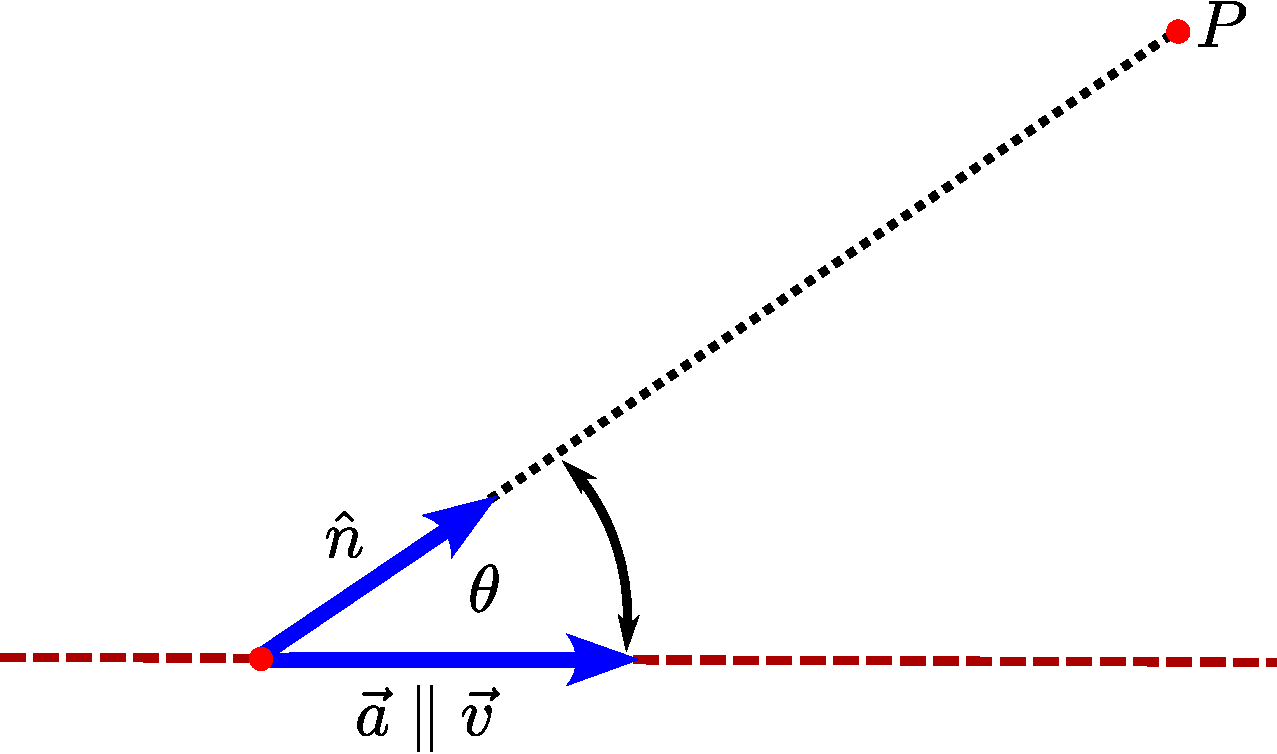
\psfig{file=fig/fig-movimiento_lineal.pdf,height=4cm,angle=0}}
\caption{Geometr'ia para un movimiento unidimensional acelerado.}
\label{R14}
\end{figure}
En este caso de movimiento unidimensional acelerado tenemos que la velocidad es paralela a la aceleraci'on, de modo que $\vec{\beta}\times\vec{a}=\vec{0}$. Adem'as,
$\hat{n}\cdot\vec{\beta}=\beta\cos\theta$.
Reemplazando esto en \eqref{dP'} encontramos que 
\begin{equation}
\frac{dP'}{d\Omega}=\frac{q^2\mu}{16\pi^2 c}\frac{\sen^2
\theta}{\left(1-\beta\cos\theta\right)^5}. \label{dppdO}
\end{equation}
\begin{figure}[H]
\centerline{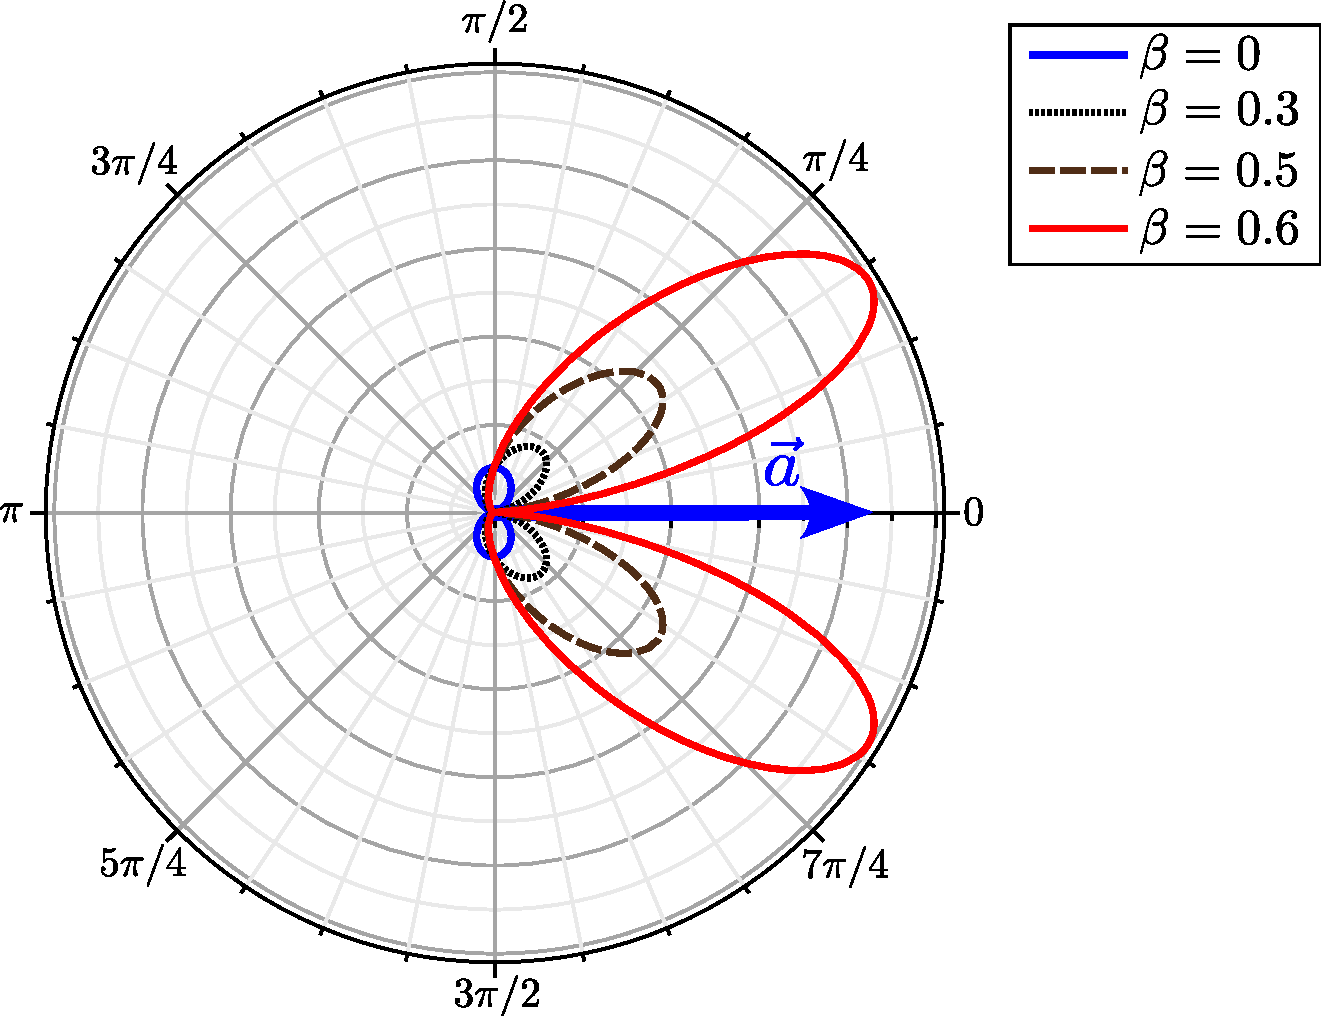
\psfig{file=fig/fig-carga-relativista.pdf,height=7cm}}
\caption{L'obulos de radiaci'on para una carga relativista acelerada. Suponemos
iguales aceleraciones y normalizamos con respecto a ${q^2\mu}/{16\pi^2 c}$. C'odigo Python \href{https://github.com/gfrubi/electrodinamica/blob/master/figuras-editables/fig-carga-relativista.py}{aqu\'i}.}
\label{lobulo02}
\end{figure}
Podemos encontrar el 'angulo $\theta=\theta_{\rm max}$ en el que se emite el
\textit{m'aximo de radiaci'on}. Derivando (\ref{dppdO}) con respecto a $\theta$ e
igualando a cero, encontramos que
\begin{equation}
\cos\theta_{\rm max}=\frac{1}{3\beta}\left\{  \sqrt{1+15\beta^2}-1\right\}  .
\end{equation}
Esto indica que, para la misma aceleraci'on, la radiaci'on emitida por una carga se concentra m'as y m'as en la direcci'on de movimiento, a medida que la velocidad de la carga es mayor.


\section{Scattering de Thomson}
%Thomson=por carga, clasicamente elastico (igual frecuencia), intensidad indep. de frecuencia.
%Compton= igual que Thomson, pero tomando en cuenta efecto Compton = corrimiento frecuencia, para energías altas (comparables a energía en reposo de carga)
%Rayleigh=por particulas neutras pequeñas comparadas con \lambda: moleculas (aire), elastico = dipolos = intensidad depende de frec^4. Ejemplo, difusión de luz solar en moléculas de la atmósfera.
%Mie = cuerpos neutros grandes comparados con \lambda
%Raman=inelastico, absorbe/emite energia de modos de excitación de un sólido o líquido.


%*** AGREGAR: Introducir Intensidad $I$ de radiacion (pot/area)

Si una onda electromagn'etica monocrom'atica incide
sobre una part'icula libre de carga $q$ y masa $m$, la carga acelera y
entonces emite radiaci'on. Esta radiaci'on ser'a emitida en otras
direcciones respecto de la direcci'on de la onda incidente. Adem'as, si la carga se mueve a velocidades no-relativistas la radiaci'on emitida por esta carga tendr'a \textit{casi exclusivamente} la misma frecuencia que la radiaci'on incidente (ver secci'on \ref{sec:rfp} para mayores detalles). El proceso completo puede ser descrito como \textit{scattering} (dispersi'on) \textit{esl'astico} de la radiaci'on incidente, que llamamos scattering de Thomson\footnote{Joseph John Thomson (1856-1940): f'isico brit'anico. Ver \url{http://es.wikipedia.org/wiki/Joseph_John_Thomson}.}.

La potencia instant'anea radiada es dada por (\ref{Lardif}) o, introduciendo el
\textit{vector de polarizaci'on $\vec{\epsilon}$ de la onda emitida} (que es, por definici'on el vector paralelo a la direcci'on del campo el'ectrico radiado, ver figura \ref{fig:natheta}):
\begin{equation}
\frac{dP}{d\Omega}=\frac{q^2\mu}{16\pi^2 c}|\vec{\epsilon}\cdot\vec{a}|^2.
\end{equation}
En este caso, la aceleraci'on es producida por la fuerza que la onda incidente ejerce sobre la carga. Si la onda incidente es \textit{plana y polarizada linealmente}, con vector de onda $\vec{k}_0$ y vector de polarizaci'on $\vec{\epsilon}_0$, su campo el'ectrico puede ser descrito usando
\begin{equation}
\vec{E}_0(\vec{x},t)=\operatorname{Re}\left[
\vec{\epsilon}_0E_0e^{i(\vec{k}_0\cdot\vec{x}-\omega t)}\right] .
\end{equation}
Suponiendo que la velocidad de la carga es en todo momento mucho menor que la de la
luz, podemos despreciar el t'ermino dependiente del campo magn'etico en la fuerza de Lorentz. Entonces, la aceleraci'on de la carga es proporcional al campo el'ectrico de la onda incidente:
\begin{equation}
\frac{d^2\vec{x}}{dt^2}
=\operatorname{Re}\left[\frac{qE_0}{m}\vec{\epsilon}_0e^{i(\vec{k}_0\cdot\vec{x}(t)
-\omega t)}\right] .
\end{equation}
Considerando las condiciones iniciales $\vec{x}(0)=\vec{0}$ y $\vec{v}(0)=\vec{0}$, integramos esta ecuaci'on y obtenemos que la posici'on y velocidad de la carga tienen la forma
\begin{equation}
\vec{x}(t)
=\operatorname{Re}\left[-\frac{qE_0}{m\omega^2}\vec{\epsilon}_0(e^{-i\omega t}-1)\right] ,
\end{equation}
\begin{equation}
\vec{v}(t)
=\operatorname{Re}\left[i\frac{qE_0}{m\omega}\vec{\epsilon}_0e^{-i\omega t}\right] .
\end{equation}
Vemos de aqu'i que las amplitudes de las oscilaciones en posici'on y velocidad son
$A={qE_0}/{m\omega^2}$ y $v_{\max}={qE_0}/{m\omega}$. Por lo
tanto, la aproximaci'on usada es consistente s'olo si $v_{\max}\ll c$, es decir si
$E_0\ll {m\omega c}/{q}$. Ya que $A={v_{\max}}/{\omega}$, esta condici'on
es equivalente a $A\ll c/\omega=\lambda/2\pi$, es decir, a que \textit{la amplitud de la oscilaci'on de la carga sea mucho menor que la longitud de onda (reducida) de la radiaci'on incidente}.

Es conveniente calcular el flujo de energ'ia promedio irradiado en un ciclo,
para lo cual requerimos el promedio $\left\langle
{dP}/{d\Omega}\right\rangle$ en un periodo:
\begin{eqnarray}
\left\langle\frac{dP}{d\Omega}\right\rangle  &=&
\frac{q^2\mu}{16\pi^2 c}\left\langle |\vec{\epsilon}\cdot\vec{a}|^2\right\rangle \\
&=&\left(\frac{q^2\mu}{16\pi^2 c}\right)\left(\frac{qE_0}{m}\right)^2\left|
\vec{\epsilon}\cdot\vec{\epsilon}_0\right|^2\left\langle
\cos^2(\omega t)\right\rangle \\
&=&\left(\frac{q^4\mu E_0^2}{32\pi^2 c m^2}\right)\left|
\vec{\epsilon}\cdot\vec{\epsilon}_0\right|^2\\
&=&\left(\frac{q^2\mu}{4\pi m}\right)^2\left(\frac{E_0^2}{2\mu c}\right) \left|
\vec{\epsilon}\cdot\vec{\epsilon}_0\right|^2.
\end{eqnarray}
En la pr'actica es conveniente describir este proceso de scattering por medio de
la correspondiente  \textit{secci'on diferencial de scattering}:
\begin{equation}
\frac{d\sigma}{d\Omega}:=\frac{\left( \text{Energ'ia promedio radiada por unidad
de tiempo y de 'angulo s'olido}\right) }{\left( \text{Energ'ia promedio
incidente por unidad de 'area y de tiempo}\right) }=\frac{\left\langle
\frac{dP}{d\Omega}\right\rangle}{\left\langle S_0\right\rangle}.
\end{equation}
Note que ${d\sigma}/{d\Omega}$ tiene unidades de 'area (por unidad de 'angulo
s'olido).
El flujo de energ'ia incidente promedio es precisamente el vector de Poynting
del campo incidente, promediado en un periodo, y est'a dado por la expresi'on \eqref{Sprom}:
\begin{eqnarray}
\left\langle S_0\right\rangle &=&\frac{1}{2\mu c}E_0^2.
\end{eqnarray}
Obtenemos entonces que la secci'on diferencial de scattering es dada por
\begin{equation}
\boxed{\frac{d\sigma}{d\Omega}  =\left(\frac{q^2\mu}{4\pi m}\right)^2\left|
\vec{\epsilon}\cdot\vec{\epsilon}_0\right|^2 .}\label{seeT}
\end{equation}
La cantidad $r_q:={q^2\mu}/{4\pi m}=(1/{4\pi\varepsilon})({q^2}/{mc^2})$ tiene dimensiones de longitud, y juega el rol de ``\textit{tama\~no efectivo}'' de la carga para el proceso de scattering considerado\footnote{Compare, por ejemplo, con la secci'on diferencial de scaterring de una esfera de radio $R$ impactada por peque\~nas part'iculas de prueba (de masa despreciable): $d\sigma/d\Omega=R^2/4$, $\sigma=\pi R^2$.}. Por ejemplo, para el electr'on en el vac'io $r_{\rm e}=(1/{4\pi\varepsilon_0})({e^2}/{m_{\rm e}c^2})\approx 2,8\times 10^{-15}m$. Esta distancia caracter'istica (de la interacci'on electromagn'etica) del electr'on es llamada \textit{radio cl'asico del electr'on}.

Para evaluar (\ref{seeT}) requerimos de una expresi'on expl'icita para
$\vec{\epsilon}$. El c'alculo es m'as sencillo si elegimos los ejes coordenados de modo que el vector de onda inicial $\vec{k}_0$ sea paralelo al eje $z$ y el vector $\epsilon_0$ paralelo al eje $x$. Ver figura \ref{fig:thomson}. En este caso, podemos escribir, $\vec{k}_0=k_0\hat{z}$, 
\begin{equation}\label{epsilon0}
\vec\epsilon_0=\hat{x},
\end{equation}
y 
\begin{equation}
\hat{n}=\hat{x}\sen\theta\cos\varphi + \hat{y}\sen\theta\sen\varphi +\hat{z}\cos\theta, \label{ene}
\end{equation}
de modo que $\theta$ es el 'angulo entre $\hat{n}$ y $\vec{k}_0$, es decir, el
\textit{'angulo de scattering} entre la radiaci'on incidente y la emitida, y $\varphi$ es el 'angulo azimutal entre $\vec{\epsilon}_0$ y
$\hat{n}$.
\begin{figure}[H]
\centerline{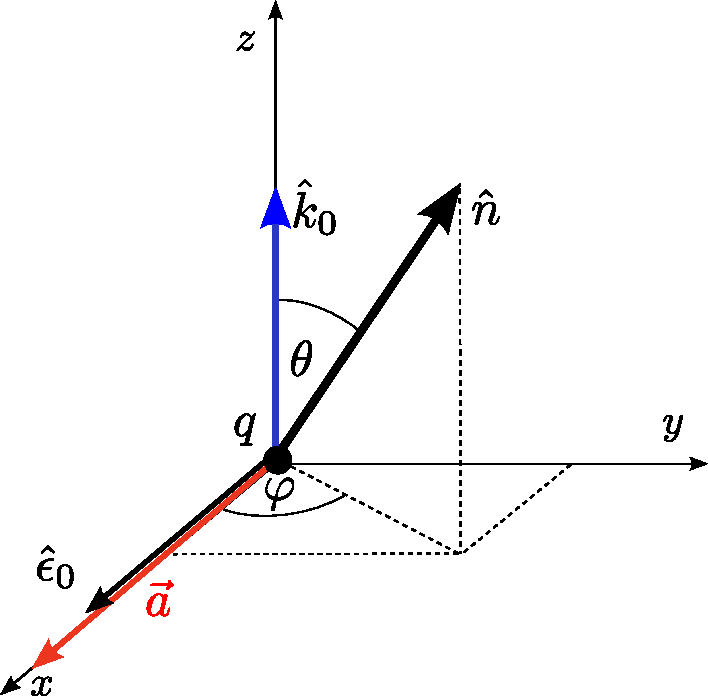
\psfig{file=fig/fig-thomson-esquema.pdf,height=5cm}}
 \caption{Esquema para el scattering Thomson.}
\label{fig:thomson}
\end{figure}
Sabemos que (la componente radiativa d)el campo el'ectrico producido por la carga es paralelo a
$\hat{n}\times(\hat{n}\times\vec{a})\propto
\hat{n}\times(\hat{n}\times\vec{\epsilon}_0)$, por lo que podemos escribir
\begin{equation}
\vec{\epsilon}:=\frac{\vec{V}}{|\vec{V}|}, \qquad
\vec{V}:=\hat{n}\times(\hat{n}\times\vec{\epsilon}_0).
\end{equation}
Al calcular $\vec{V}$ usando de \eqref{epsilon0} y \eqref{ene} encontramos que
\begin{equation}
\vec{V}=-\hat{x}(\cos^2\theta+\sen^2\theta\sen^2\varphi)+\hat{y}\sen^2\theta\sen\varphi\cos\varphi
+\hat{z}\sen\theta\cos\theta\cos\varphi,
\end{equation}
y por lo tanto
\begin{equation}
|\vec{V}|=\sqrt{\sen^2\varphi+\cos^2\theta\cos^2\varphi}.
\end{equation}
As'i, obtenemos
\begin{eqnarray}
 \vec{\epsilon}\cdot\vec{\epsilon}_0&=&\frac{1}{|\vec{V}|}
\vec{V}\cdot\vec{\epsilon}_0 \\
 &=& -\frac{1}{|\vec{V}|}\left(\sen^2\varphi+\cos^2\theta\cos^2\varphi \right) \\
  &=&-\sqrt{\sen^2\varphi+\cos^2\theta\cos^2\varphi} .
\end{eqnarray}
Por lo tanto,
\begin{equation}
\frac{d\sigma}{d\Omega}=\left(\frac{q^2\mu}{4\pi m}\right)^2
\left(\sen^2\varphi+\cos^2\theta\cos^2\varphi \right).
\end{equation}
Recuerde que $\theta$ es el 'angulo de scattering y $\varphi$ es el 'angulo
azimutal entre la polarizaci'on inicial y la direcci'on de la radiaci'on
emitida.

Para radiaci'on incidente \textit{no polarizada}, podemos considerar que la
mitad de la radiaci'on tiene una polarizaci'on descrita por un 'angulo $\varphi$
y la otra mitad est'a polarizada en la direcci'on perpendicular, es decir,
correspondiente a cambiar el 'angulo $\varphi$ por ${\pi}/{2}-\varphi$, ver figura  \ref{fig:thomson}. De este modo, la secci'on diferencial de scattering es dada, en este caso, por
\begin{align}
\left. \frac{d\sigma}{d\Omega}\right|_{\rm no-pol}&=\frac{1}{2}\left[\left.
\frac{d\sigma}{d\Omega}\right|_\varphi+\left.
\frac{d\sigma}{d\Omega}\right|_{\frac{\pi}{2}-\varphi}\right] \\
&=\frac{1}{2}\left(\frac{q^2\mu}{4\pi m}\right)^2\left[\sen^2\varphi+\cos^2\theta\cos^2\varphi
+\sen^2\left(\frac{\pi}{2}-\varphi\right)+\cos^2\theta\cos^2\left(\frac{\pi}{2}-\varphi\right)\right] \\
&=\frac{1}{2}\left(\frac{q^2\mu}{4\pi m}\right)^2\left[\sen^2\varphi+\cos^2\theta\cos^2\varphi
+\cos^2\varphi+\cos^2\theta\sen^2\varphi\right].
\end{align}
Como era de esperar, en este caso obtenemos una secci'on diferencial de scattering independiente de $\varphi$:
\begin{equation}
\boxed{\frac{d\sigma}{d\Omega}=\left(\frac{q^2\mu}{4\pi m}\right)^2\frac{1}
{2}\left(  1+\cos^2\theta\right) .}
\end{equation}
\begin{figure}[H]
\centerline{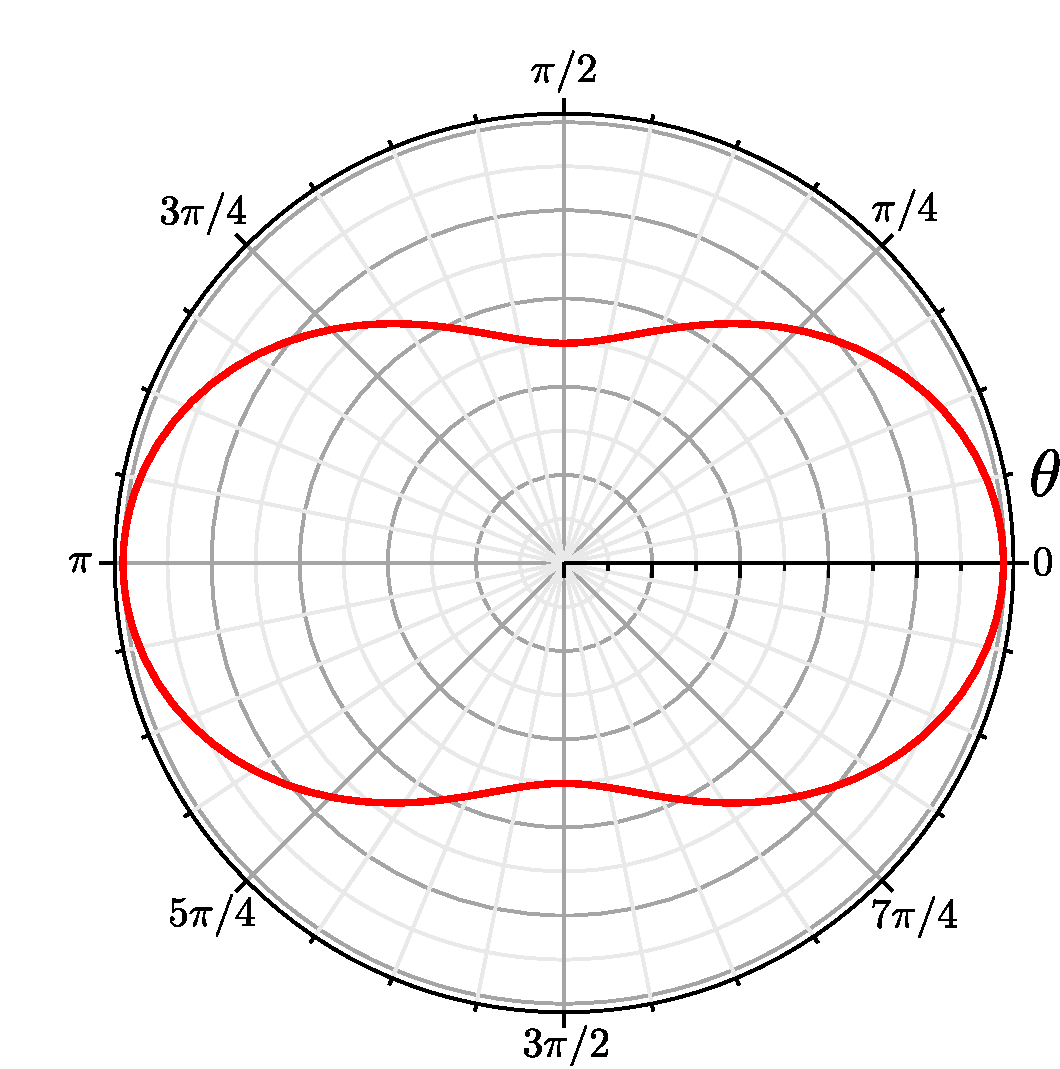
\psfig{file=fig/fig-thomson2d.pdf,height=5cm}}
 \caption{Secci\'on diferencial de scattering $d\sigma/d\Omega$ en funci'on de $\theta$ en el plano $z-x$.}
\label{fig:thomson_2d}
\end{figure}
'Esta es la llamada \textit{f'ormula de Thomson} para scattering de radiaci'on
por cargas libres, y es apropiada para describir muchas situaciones f'isicas, com por ejemplo \textit{scattering de rayos X
no-polarizados por electrones}, o \textit{rayos gamma por protones}. 
La distribuci'on angular se muestra en la figura \ref{fig:thomson_2d}. 

La \textit{secci'on total de scattering}, definida en general como la integral sobre el 'angulo s'olido de la secci'on diferencial, es llamada en este caso \textit{secci'on tranversal de Thomson}, y es dada por
\begin{equation}
\boxed{\sigma_{T}=\frac{8\pi}{3}\left(\frac{q^2\mu}{4\pi m}\right)^2=\frac{8\pi}{3} r_q^2.}
\end{equation}

Para el caso de electrones, la secci'on tranversal total de Thomson tiene el valor $\sigma_{T}\approx 6.65\times 10^{-29}$ m$^2$ y $r_q\approx 2.82\times 10^{-15}$ m es el llamado \textit{radio cl'asico del electr'on}.

\subsection{Correcciones a la f'ormula de Thomson*}
La f'ormula cl'asica de Thomson se ajusta a las observaciones s'olo para frecuencias bajas, donde el momentum del fot'on incidente puede ser ignorado. Cuando los momenta $\hbar\omega/c$ de los fotones son comparables o mayores que $mc$, es necesario incluir algunas modificaciones al modelo sencillo aqu'i expuesto. Uno de estos efectos a tomar en cuenta es el efecto Compton, por el que la frecuencia (energ'ia) de un fot'on dispersado es menor que la frecuencia (energ'ia) del incidente, ya que la carga necesariamente sufre de un ``recoil'' durante el proceso. La cinem'atica (relativista) predice que el cambio de vector de onda de la radiaci'on es de la forma
\begin{equation}
\frac{k'}{k}=\frac{1}{1+\frac{\hbar\omega}{mc^2}\left(  1-\cos
\theta\right)  }, \label{Thomson}
\end{equation}
donde $\theta$ es el 'angulo de scattering en la sistema laboratorio (el marco
de referecia en reposo con la carga blanco). Un c'alculo cu'antico del
scattering de fotones por part'iculas de carga $q$ y masa $m$ produce la seccion
transversal siguiente:
\begin{equation}
\frac{d\sigma}{d\Omega}=\left(\frac{q^2\mu}{4\pi m}\right)^2  \left(
\frac{k'}{k}\right)^2\left|  \vec{\epsilon}\cdot\vec{\epsilon}_0\right|
^2 , \label{Thomson-corr}
\end{equation}
en lugar de la expresi'on cl'asica. El factor $(k'/k)^2$ describe una
reducci'on  (respecto al resultado cl'asico de Thomson) de la energ'ia radiada
para 'angulos grandes, como se muestra en las curvas segmentadas en la figura.
Adem'as, existen correcciones adicionales para el scattering fot'on-electr'on al
tomar en cuenta el spin ${1}/{2}$ del electr'on (descrito, por ejemplo, por
la ecuaci'on de Dirac). Las curvas son similares a las del caso de part'iculas
sin spin, pero las secciones son un poco mayores para 'angulos grandes debido a
la contribuci'on del momento magn'etico del electr'on.

\begin{figure}[!h]
\centerline{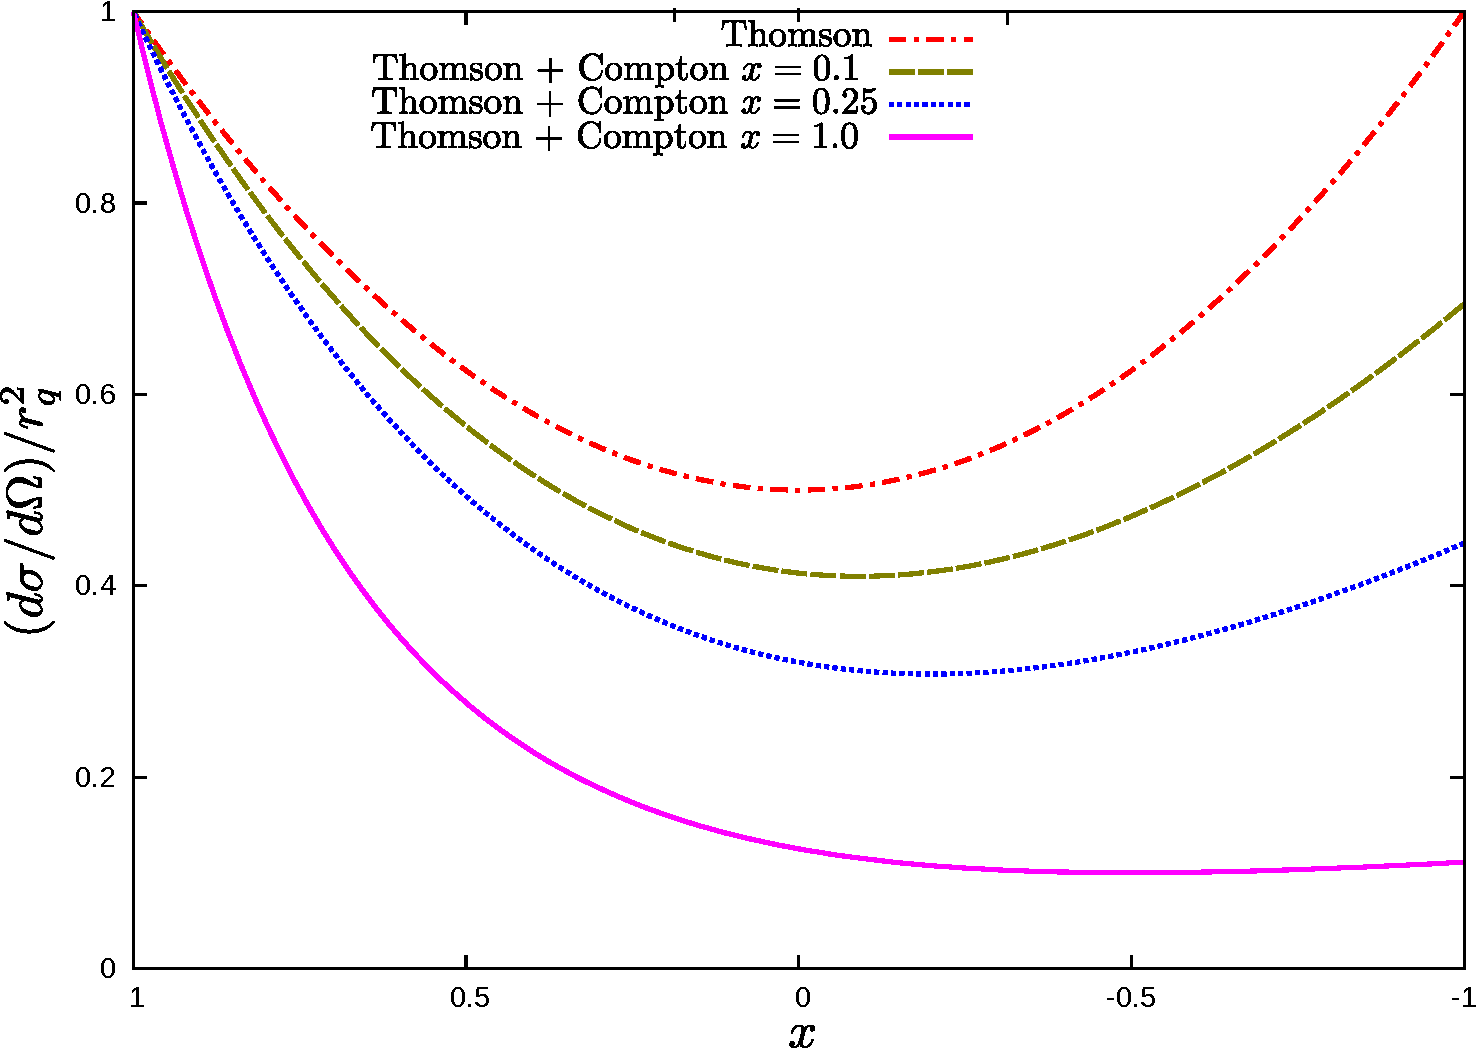
\psfig{file=fig/fig-thomson.pdf,height=5cm}}
 \caption{Secci'on diferencial de scattering Thomson (\ref{Thomson}) y
correcciones cu'antico-relativistas (\ref{Thomson-corr}). El gr'afico muestra
${d\sigma}/{d\Omega}$ en unidades de $r_q^2$ en funci'on de
$\cos\theta$ para distintos valores de $x:={\hbar\omega}/{mc^2}$.}
\label{thomson}
\end{figure}

Nota: Adem'as existe una expresi'on que incluye correcciones relativistas y de la interacci'on de la radiaci'on con el momentum magn\'{e}tico del electr'on:
\begin{equation}
\frac{d\sigma }{d\Omega}=\frac{1}{2}\left(\frac{q^2\mu}{4\pi m}\right)^2
\left(  \frac{1}{1+x\left(  1-\cos
\theta\right)  }\right)  ^{2}\left(  1+\cos^{2}\theta+\frac{x^{2}\left(
1-\cos\theta\right)  ^{2}}{1+x\left(  1-\cos\theta\right)  }\right),
\end{equation}
donde $x:={\hbar\omega}/{mc^{2}}$. La expresi'on anterior es la llamada \textit{f'ormula de Klein-Nishina}, que puede ser calculada en el contexto de la teor'ia Cu'antica de Campos del campo electromagn'etico interactuando con fermiones de spin 1/2 conocida como \textit{electrodin'amica cu'antica}.
La secci'on eficaz total de scattering de acuerdo a la f'ormula de Klein-Nishina es
\begin{equation}
 \sigma(x)=\frac{3}{4}\sigma_T\left[\frac{(1+x)}{x^3}\left\lbrace\frac{2x(1+x)}{1+2x}-\ln(1+2x)\right\rbrace+\frac{1}{2x}\ln(1+2x)-\frac{1+3x}{(1+2x)^2}\right].
\end{equation}



%
%  Nosotros solo trabajamos con los limites de
% la expresion para $\hbar\omega\ll mc^2$ y $\hbar\omega\gg mc^2$%
% \begin{equation}
% \frac{\sigma}{\sigma_{T}}=\left\{
% \begin{array}
% [c]{c}%
% 1-2\frac{\hbar\omega}{mc^2}+...\text{ }\hbar\omega\ll mc^2\\
% \frac{3}{4}\frac{mc^2}{\hbar\omega}\text{ }\hbar\omega\gg mc^2%
% \end{array}
% \right.
% \end{equation}
% Para scattering por electrones el limite de frecuencia baja es el mismo, pero
% altas frecuencias hay un factor multiplicativo adicional $\frac{1}{4}+\frac
% {1}{2}\ln\left(  2\hbar\omega/mc^2\right)  .$
%
% Para protones la salida desde la formula de Thomson ocurre para energias de
% fotones sobre 100 MeV aproximadamente. Esto es lejos bajo la energia critica
% $\hbar\omega\sim Mc^2\sim1$GeV,



\section{Distribuci'on de Energ'ia en 'Angulo y Frecuencia, radiada
por cargas aceleradas}

Hab'iamos obtenido, ver \eqref{Pinf1} y \eqref{S2E}, que la potencia irradiada por unidad de 'angulo s'olido es dada en general por
\begin{equation}\label{dp1}
\frac{dP}{d\Omega}(\hat{n},t)=\lim_{r\to\infty}\frac{1}{\mu c}\left|r\vec{E}_{\rm{rad}}(\vec{x},t)\right|^2 , %=\left|  \vec{\cal A}(t,\hat{n})\right|  _{\rm ret}^2, 
\end{equation}
donde $\vec{E}_{\rm{rad}}$ es el campo el'ectrico radiativo.
%
%Introduciremos el campo vectorial auxiliar $\vec{\cal A}(\hat{n},t)$, definido por
%\begin{equation}
%\vec{\cal A}(\hat{n},t):=\frac{1}{\sqrt{\mu c}} \lim_{r\to\infty}\left(r\vec{E}_{\rm{rad}}(\vec{x},t)\right).
%\label{dp2}
%\end{equation}
%\begin{equation}
%\vec{\cal A}(\hat{n},t):=\frac{1}{\sqrt{\mu c}} \lim_{r\to\infty}\left(r\vec{E}_{\rm{rad}}\right)_{\rm ret}=\sqrt{\frac{q^2\mu}{16\pi^2
%c}}\lim_{r\to\infty}\left.\frac{\hat{n}\times\left[ \left( \hat{n}-\vec{\beta}\right)
%\times{\vec{a}}\right] }{\left( 1-\vec{\beta}\cdot\hat{n}\right)
%^3}\right|_{\rm ret}.
%\label{dp2}
%\end{equation}
La energ'ia total irradiada por unidad de 'angulo s'olido es entonces
\begin{equation}
\frac{dE}{d\Omega}(\hat{n}) =\frac{1}{\mu c}\int_{-\infty}^{\infty}\lim_{r\to\infty}\left|r\vec{E}_{\rm{rad}}(\vec{x},t)\right|^2 dt .
\end{equation}
%\begin{equation}
%\frac{dE}{d\Omega}(\hat{n}) =\int_{-\infty}^{\infty}\frac{dP}{d\Omega}(\hat{n})\,dt
%=\int_{-\infty}^{\infty}\left|  \vec{\cal A}(\hat{n},t)  \right|^2dt .
%\end{equation}
Queremos estudiar el \textit{espectro} de la radiaci'on emitida, es decir, \textit{la distribuci'on de potencia para distintas frecuencias}. Para ello, podemos \textit{expresar el campo radiado en t'erminos de oscilaciones peri'odicas}. Esto significa expresar el campo el'ectrico como una superposici'on de funciones arm'onicas, por medio de la transformada de Fourier $\tilde{\vec{E}}(\vec{x},\omega)$ del vector $\vec{E}(\vec{x},t)$, de modo que
\begin{equation}
 \vec{E}(\vec{x},t)=\frac{1}{\sqrt{2\pi}}\int_{-\infty}^{\infty}\tilde{\vec{E}}
(\vec{x},\omega) e^{i\omega t}d\omega ,
\end{equation}
%\begin{equation}
% \vec{\cal A}(\hat{n},t)=\frac{1}{\sqrt{2\pi}}\int_{-\infty}^{\infty}\vec{\cal
%A}(\omega) e^{i\omega t}d\omega ,
%\end{equation}
donde
\begin{equation}
\tilde{\vec{E}}(\vec{x},\omega) :=\frac{1}{\sqrt{2\pi}}\int_{-\infty}^{\infty}\vec{E}(\vec{x},t) e^{-i\omega t}dt .  \label{dp3}
\end{equation}
%\begin{equation}
%\vec{E}(\hat{n},\omega) :=\frac{1}{\sqrt{2\pi}}\int_{-\infty}^{\infty}\vec{\cal
%A}(t) e^{-i\omega t}dt .  \label{dp3}
%\end{equation}

El hecho que %$\vec{\cal A}(\hat{n},t)$ 
$ \vec{E}(\vec{x},t)$ es real se traduce en que 
%$\vec{\cal A}(\hat{n},-\omega)=\vec{\cal A}^*(\hat{n},\omega)$
$\tilde{\vec{E}}^*(\vec{x},\omega)=\tilde{\vec{E}}(\vec{x},-\omega)$. En t'erminos de la transformada de 
%$\vec{\cal A}(\hat{n},t)$
$ \vec{E}(\vec{x},t)$, la energ'ia total radiada por unidad de 'angulo s'olido puede escribirse como:
\begin{eqnarray}
\frac{dE}{d\Omega}(\hat{n}) &=&\frac{1}{\mu c}\lim_{r\to\infty} \int_{-\infty}^{\infty}r^2\left|\vec{E}(\vec{x},t)
\right|^2dt \label{dEdO0}\\
&=&\frac{1}{\mu c}\lim_{r\to\infty}\int_{-\infty}^{\infty}r^2\vec{E}(\vec{x},t)\cdot \vec{E}^*(\vec{x},t)dt\\
&=&\frac{1}{2\pi}\frac{1}{\mu c}\lim_{r\to\infty}\int_{-\infty}^{\infty}\int_{-\infty}^{\infty}\int_{-\infty}^{
\infty}r^2\tilde{\vec{E}}(\vec{x},\omega) \cdot e^{i\omega t}\tilde{\vec{E}}^\ast(\vec{x},\omega')e^{-i\omega' t}\,d\omega d\omega' dt\\
&=&\frac{1}{2\pi}\frac{1}{\mu c}\lim_{r\to\infty} \int_{-\infty}^{\infty}\int_{-\infty}^{\infty}r^2\vec{E}(\vec{x},\omega)\cdot \vec{E}^*(\vec{x},\omega')\int_{-\infty}^{\infty} e^{i(\omega-\omega')t}\,dtd\omega d\omega' .
\end{eqnarray}
%\begin{eqnarray}
%\frac{dE}{d\Omega}(\hat{n}) &=&\int_{-\infty}^{\infty}\left|\vec{\cal A}(t)
%\right|^2dt \label{dEdO0}\\
%&=&\int_{-\infty}^{\infty}\vec{\cal A}(\hat{n},t)\cdot \vec{\cal A}^*(\hat{n},t)dt\\
%&=&\frac{1}{2\pi}\int_{-\infty}^{\infty}\int_{-\infty}^{\infty}\int_{-\infty}^{
%\infty}\vec{\cal A}(\hat{n},\omega) \cdot e^{i\omega t}\vec{\cal A}^\ast\left(\hat{n},\omega'\right)e^{-i\omega' t}\,d\omega d\omega' dt\\
%&=&\frac{1}{2\pi} \int_{-\infty}^{\infty}\int_{-\infty}^{\infty}\vec{\cal A}(\hat{n},\omega)\cdot \vec{\cal A}^*(\hat{n},\omega')\int_{-\infty}^{\infty} e^{i(\omega-\omega')t}\,dtd\omega d\omega' .
%\end{eqnarray}
Recordando que
\begin{equation}
\frac{1}{2\pi}\int_{-\infty}^{\infty }e^{i\left((  k-k' \right)  x}dx=
\delta\left(  k-k' \right),
\end{equation}
llegamos a que
\begin{eqnarray}
\frac{dE}{d\Omega}(\hat{n})
&=&\frac{1}{\mu c}\lim_{r\to\infty}\int_{-\infty}^{\infty}\int_{-\infty}^{\infty} r^2\tilde{\vec{E}}(\vec{x},\omega)\cdot\tilde{\vec{E}}^\ast(\vec{x},\omega') \delta (\omega-\omega')  d\omega d\omega'\\
&=&\frac{1}{\mu c}\lim_{r\to\infty}\int_{-\infty}^{\infty}r^2\left|\tilde{\vec{E}}(\vec{x},\omega)\right|^2 d\omega. \label{dedO1}
\end{eqnarray}
%\begin{eqnarray}
%\frac{dE}{d\Omega}(\hat{n})
%&=&\int_{-\infty}^{\infty}\int_{-\infty}^{\infty}\vec{\cal A}(\hat{n},\omega)\cdot
%\vec{\cal A}^\ast(\hat{n},\omega') \delta (\omega-\omega')  d\omega d\omega'\\
%&=&\int_{-\infty}^{\infty}\left|\vec{\cal A}(\hat{n},\omega)\right|^2 d\omega. \label{dedO1}
%\end{eqnarray}
Note que la igualdad entre las expresiones (\ref{dEdO0}) y (\ref{dedO1}) no es m'as que el resultado usualmente conocido como \textit{teorema de Parceval}.

Definimos la\textit{ energ'ia radiada por unidad de 'angulo s'olido y por intervalo de frecuencia (angular)} ${d^2E}/{d\Omega d\omega}$, de modo que
\begin{equation}
\frac{dE}{d\Omega}(\hat{n})=\int_0^{\infty}\frac{d^2E}{d\Omega d\omega}(\hat{n},\omega)\,d\omega .
\end{equation}
Con esta definici'on y el resultado (\ref{dedO1}), encontramos
\begin{equation}
\frac{d^2E}{d\Omega d\omega}(\hat{n},\omega)=\frac{1}{\mu c}\lim_{r\to\infty}r^2\left[\left|\tilde{\vec{E}}(\vec{x},\omega)\right|^2 +\left|\tilde{\vec{E}}(\vec{x},-\omega)\right|^2\right]
=\frac{2}{\mu c}\lim_{r\to\infty}r^2\left|\tilde{\vec{E}}(\vec{x},\omega)\right|^2.
\end{equation}
En el caso de la radiaci'on de una carga acelerada, tenemos
\begin{equation}
\tilde{\vec{E}}(\vec{x},\omega)= \frac{1}{\sqrt{2\pi}}\frac{q\mu}{4\pi}\int_{-\infty}^{\infty
}\left.\frac{\hat{n}\times\left[ \left( \hat{n}-\vec{\beta}\right)
\times{\vec{a}}\right] }{R\left( 1-\vec{\beta}\cdot\hat{n}\right)
^3}\right|_{\rm ret}e^{-i\omega t}dt .
\end{equation}
%\begin{equation}
%\vec{\cal A}(\hat{n},\omega)= \sqrt{\frac{q^2\mu}{32\pi^3c}}\int_{-\infty}^{\infty
%}\left.\frac{\hat{n}\times\left[ \left( \hat{n}-\vec{\beta}\right)
%\times{\vec{a}}\right] }{\left( 1-\vec{\beta}\cdot\hat{n}\right)
%^3}\right|_{\rm ret}e^{-i\omega t}dt .
%\end{equation}
Para simplificar la integral introducimos la nueva variable de integraci'on
$t':=t_{\rm ret}(t)=t-{R}/{c}$ y usamos (\ref{dtt'2}), de modo que podemos escribir
\begin{eqnarray}
\tilde{\vec{E}}(\vec{x},\omega)&=&\frac{1}{\sqrt{2\pi}}\frac{q\mu}{4\pi}\int_{-\infty}^{\infty
}\left.\frac{\hat{n}\times\left[ \left( \hat{n}-\vec{\beta}\right)
\times{\vec{a}}\right] }{R\left( 1-\vec{\beta}\cdot\hat{n}\right)
^3}\right|_{t'}e^{-i\omega (t'+R(t')/c)}\left(
1-\vec{\beta}\cdot\hat{n}\right) dt' \\
&=&\frac{1}{\sqrt{2\pi}}\frac{q\mu}{4\pi}\int_{-\infty}^{\infty
}\left.\frac{\hat{n}\times\left[ \left( \hat{n}-\vec{\beta}\right)
\times{\vec{a}}\right] }{R\left(1-\vec{\beta}\cdot\hat{n}\right)^2}
\right|_{t'}e^{-i\omega (t'+R(t')/c)} dt' \\
&=&\frac{1}{\sqrt{2\pi}}\frac{q\mu}{4\pi}\int_{-\infty}^{\infty
}\frac{\hat{n}\times\left[ \left( \hat{n}-\vec{\beta}\right)
\times{\vec{a}}\right] }{R\left( 1-\vec{\beta}\cdot\hat{n}\right)^2}
e^{-i\omega (t+R(t)/c)} dt.
\end{eqnarray}
%\begin{eqnarray}
%\vec{\cal A}(\hat{n},\omega)&=&\sqrt{\frac{q^2\mu}{32\pi^3c}}\int_{-\infty}^{\infty
%}\left.\frac{\hat{n}\times\left[ \left( \hat{n}-\vec{\beta}\right)
%\times{\vec{a}}\right] }{\left( 1-\vec{\beta}\cdot\hat{n}\right)
%^3}\right|_{t'}e^{-i\omega (t'+R(t')/c)}\left(
%1-\vec{\beta}\cdot\hat{n}\right) dt' \\
%&=&\sqrt{\frac{q^2\mu}{32\pi^3c}}\int_{-\infty}^{\infty
%}\left.\frac{\hat{n}\times\left[ \left( \hat{n}-\vec{\beta}\right)
%\times{\vec{a}}\right] }{\left(1-\vec{\beta}\cdot\hat{n}\right)^2}
%\right|_{t'}e^{-i\omega (t'+R(t')/c)} dt' \\
%&=&\sqrt{\frac{q^2\mu}{32\pi^3c}}\int_{-\infty}^{\infty
%}\frac{\hat{n}\times\left[ \left( \hat{n}-\vec{\beta}\right)
%\times{\vec{a}}\right] }{\left( 1-\vec{\beta}\cdot\hat{n}\right)^2}
%e^{-i\omega (t+R(t)/c)} dt.
%\end{eqnarray}
En el 'ultimo paso hemos renombrado la variable de integraci'on volviendo
nuevamente a denotarla por $t$. Esta integral es evaluada en ``en el infinito'', es decir, a grandes distancias de la carga ($r\rightarrow\infty$). Tomando en cuenta esto, podemos expandir $R$ en potencias de ${\vec{z}}/{r}$, obteniendo
\begin{equation}
R(t)  =r-\vec{z}(t) \cdot\hat{n}+O\left(\left[z/r\right]^2\right). \label{expR} %aqui cambie
\end{equation}
Usando esta expansi'on, podemos escribir:
\begin{equation}
\tilde{\vec{E}}(\vec{x},\omega)=\frac{1}{\sqrt{2\pi}}\frac{q\mu}{4\pi}\frac{e^{-i\frac{\omega r}{c}}}{r}\int_{-\infty}^{\infty}\frac{\hat{n}\times\left[ \left( \hat{n}-\vec{\beta}\right)
\times{\vec{a}}\right] }{\left( 1-\vec{\beta}\cdot\hat{n}\right)^2}
e^{-i\omega (t-\vec{z}(t)\cdot\hat{n}/c+O([z/r]^2))} dt,
\end{equation}
%\begin{equation}
%\vec{\cal A}(\hat{n},\omega)=\sqrt{\frac{q^2\mu}{32\pi^3c}}e^{-i\frac{\omega
%r}{c}}\int_{-\infty}^{\infty}\frac{\hat{n}\times\left[ \left( \hat{n}-\vec{\beta}\right)
%\times{\vec{a}}\right] }{\left( 1-\vec{\beta}\cdot\hat{n}\right)^2}
%e^{-i\omega (t-\vec{z}(t)\cdot\hat{n}/c+O([z/r]^2))} dt,
%\end{equation}
y, por lo tanto, la energ'ia total irradiada por unidad de 'angulo s'olido e
intervalo de frecuencia es (en el l'imite $r\to\infty$)
\begin{equation}\marginnote{Distribuci'on de energ'ia en frecuencia}
\boxed{\frac{d^2E}{d\Omega d\omega}(\hat{n},\omega)
=\frac{q^2\mu}{16\pi^3c}\left|\int_{-\infty}^{\infty
}\frac{\hat{n}\times\left[ \left( \hat{n}-\vec{\beta}\right)
\times{\vec{a}}\right] }{\left( 1-\vec{\beta}\cdot\hat{n}\right)^2}
e^{-i\omega (t-\vec{z}(t)\cdot\hat{n}/c)} dt\right|^2 .} \label{dEdOdo}
\end{equation}
En general, \textit{una carga en un movimiento arbitrario irradiar'a en un continuo de frecuencias}. Esto se refleja en que ${d^2E}/{d\Omega d\omega}$ ser'a una cierta funci'on continua de la frecuencia $\omega$ de emisi'on.

\subsection{Caso de movimiento peri'odico}\label{sec:rfp}


Si el movimiento de una carga es \textit{peri'odico}, entonces el
espectro continuo de frecuencias de la radiaci'on emitida se reduce a un
\textit{espectro discreto} conteniendo frecuencias m\'{u}ltiples de la frecuencia
fundamental.

Si el movimiento es peri'odico, con periodo $T$, la velocidad y aceleraci'on de la carga ser'an funciones peri'odicas. Como consecuencia, tambi'en $\vec{E}(\vec{x},t)$ ser'a una funci'on peri'odica en $t$, y por lo tanto es posible expresarla en t'erminos de la siguiente \textit{serie de Fourier}
\begin{equation}
\vec{E}(\vec{x},t) =\sum_{m\,\in\, \mathbb{Z}} \vec{E}_{m}(\vec{x})e^{i\omega_{m}t},
\end{equation}
donde $\omega_{m}:=m\omega_0$ ser'an m'ultiplos de la frecuencia
fundamental $\omega_0:={2\pi}/{T}$, y
\begin{equation}
\vec{E}_{m}(\vec{x}) =\frac{1}{T}\int_0^{T}\vec{E}(\vec{x},t) e^{-i\omega_{m}t}dt. \label{defAm}
\end{equation}
Debido a la periodicidad del movimiento, la energ'ia radiada entre $t=-\infty$ y $t=+\infty$ \textit{es infinita}. Esto motiva considerar, en lugar de la energ'ia  total emitida (por unidad de 'angulo s'olido), la energ'ia emitida s'olo en un periodo de la oscilaci'on o, equivalentemente, la \textit{potencia promedio} de la radiaci'on emitida \textit{en un periodo} $T$ (por unidad de 'angulo s'olido), definida por
\begin{equation}
\left\langle \frac{dP}{d\Omega}\right\rangle (\hat{n}) :=\frac{1}{T}\int_0^{T}\frac{dP}{d\Omega}(\hat{n},t)\,dt.
\end{equation}
Usando la expansi'on en serie de Fourier del vector $\vec{\cal A}$, tenemos que
\begin{align}
\left\langle \frac{dP}{d\Omega}\right\rangle (\hat{n})&
=\frac{1}{T}\int_0^{T}\lim_{r\to\infty}\frac{1}{\mu c}\left|r \vec{E}(\vec{x},t)\right|^2dt\\
&  =\frac{1}{\mu c}\lim_{r\to\infty}\frac{r^2}{T}\int_0^{T}\sum_{m}\vec{E}_{m}^*e^{-i\omega_{m}t}\cdot\sum_{m'}\vec{E}_{m'}e^{i\omega_{m'}t}dt\\
&  =\frac{1}{\mu c}\lim_{r\to\infty}\frac{r^2}{T}\sum_{m,m' }\vec{E}_{m}^*\cdot\vec{E}_{m'}e^{i\left(\omega_{m'}-\omega_{m}\right)  t}dt\\
&  =\frac{1}{\mu c}\lim_{r\to\infty}r^2 \sum_{m,m'}\vec{E}_{m}^*\cdot\vec{E}_{m'}\frac{1}{T}
\int_0^{T}e^{i\omega_0\left(m'-m\right)  t}dt\\
&  =\frac{1}{\mu c}\lim_{r\to\infty}r^2\sum_{m,m' }\vec{E}_{m}^*\cdot\vec{E}_{m' }\delta_{m,m'}\\
&  =\frac{1}{\mu c}\lim_{r\to\infty}r^2\sum_{m}\left|\vec{E}_{m}\right|^2,
\end{align}
donde hemos usado
\begin{equation}
\frac{1}{T}\int_0^{T}e^{i\omega_0\left(m'-m\right)t }dt\equiv\delta_{m,m' }.
\end{equation}
Puesto que $\vec{E}(\hat{n},t)$ es real, tendremos que $\vec{E}_{m}^*=\vec{E}_{-m}$, y entonces podemos escribir:
\begin{equation}
\left\langle\frac{dP}{d\Omega}\right\rangle (\hat{n}) =\frac{1}{\mu c}\lim_{r\to\infty}r^2\left[\left|\vec{E}_0\right|^2
+2\sum_{m=1}^{\infty}\left|\vec{E}_{m}\right|^2\right].
\end{equation}
Definimos la \textit{potencia promedio radiada por
unidad de 'angulo s'olido en el m-'esimo arm'onico} como:
\begin{equation}
\left\langle\frac{dP_{m}}{d\Omega}\right\rangle (\hat{n}) :=\frac{2}{\mu c}\lim_{r\to\infty}r^2\left|\vec{E}_{m}\right|^2, \qquad m=1,2,3,\cdots.
\end{equation}
La expresi'on (\ref{defAm}) nos permite entonces escribir, para el caso de el campo producido por una carga puntual:
\begin{eqnarray}
\left\langle \frac{dP_{m}}{d\Omega}\right\rangle (\hat{n})&=&
\frac{2}{\mu cT^2}\lim_{r\to\infty}r^2\left|\int_0^{T}\vec{E}(\vec{x},t)e^{-i\omega_{m}t}dt\right|^2\\
&=&\frac{q^2\mu}{8\pi^2T^2c}\left| \int_0^{T}\left.\frac{\hat{n}\times\left[  \left(\hat{n}-\vec{\beta}\right)\times\vec{a}\right] }{\left(
1-\vec{\beta}\cdot\hat{n}\right)^3}\right|_{\rm ret} e^{-i\omega_{m}t}dt\right|^2.
\end{eqnarray}
Procedemos ahora en forma an'aloga al caso de espectro continuo, es decir, efectuamos un cambio de variable de integraci'on para expresar la integral en t'erminos del tiempo retardado, y usamos la expansi'on (\ref{expR}). Con esto, obtenemos
\begin{eqnarray}
\left\langle \frac{dP_{m}}{d\Omega}\right\rangle (\hat{n})
  &=&\frac{q^2\mu}{8\pi^2T^2c}\left|
\int_{-{R}/{c}}^{T-{R}/{c}}\frac{\hat{n}\times\left[\left(\hat{n}-\vec{
\beta}\right)\times\vec{a}\right]}{\left(1-\vec{\beta}\cdot\hat{n}\right)^2} e^{-i\omega_{m}\left(t-\vec{z}\cdot\hat{n}/c\right)}dt \right|^2. \label{int2}
\end{eqnarray}
Adem'as, puesto que el integrando de (\ref{int2}) es peri'odico (asume los
mismos valores para $t$ y $t+T$), entonces podemos escribir
\begin{equation}
\boxed{\left\langle \frac{dP_{m}}{d\Omega}\right\rangle (\hat{n})
=\frac{q^2\mu}{8\pi^2T^2c}\left|
\int_0^{T}\frac{\hat{n}\times\left[\left(\hat{n}-\vec{\beta}\right)
\times\vec{a}\right]}{\left(1-\vec{\beta}\cdot\hat{n}\right)^2} e^{-i\omega_{m}\left(t-\vec{z}\cdot\hat{n}/c\right)}dt \right|^2, }\label{int3}
\end{equation}
que es la expresi'on an'aloga a (\ref{dEdOdo}).

Es posible reescribir (\ref{int3}) en forma m'as simple, usando la identidad
\begin{equation}
\frac{d}{dt}\left[ \frac{\hat{n}\times\left(  \hat{n}\times\vec{\beta}\right)
}{\left(  1-\vec{\beta}\cdot\hat{n}\right)  }\right] \equiv\frac{1}{c}
\frac{\hat{n}\times\left[
\left(  \hat{n}-\vec{\beta}\right)  \times\vec{a}\right]
}{\left(  1-\vec{\beta}\cdot\hat{n}\right)^2}, \label{iddt1}
\end{equation}
y efectuando una integraci'on por partes, ya que
\begin{align}
\frac{1}{c}\int_0^{T}\frac{\hat{n}\times\left[\left(\hat{n}-\vec{\beta}\right)
\times\vec{a}\right]}{\left(1-\vec{\beta}\cdot\hat{n}\right)^2} e^{-i\omega_{m}\left(t-\frac{1}{c}\vec{z}\cdot\hat{n}\right)}dt
&= \left.\frac{\hat{n}\times\left(\hat{n}\times\vec{\beta}\right)
}{\left(1-\vec{\beta}\cdot\hat{n}\right)} e^{-i\omega_{m}\left(t-\frac{1}{c}\vec{z}\cdot\hat{n}\right)  }\right|^T_0
\nonumber\\
&\quad- \int_0^{T}\frac{\hat{n}\times\left(
\hat{n}\times\vec{\beta}\right)}{\left(  1-\vec{\beta}\cdot\hat{n}\right) }
e^{-i\omega_{m}\left(t-\frac{1}{c}\vec{z}\cdot\hat{n}\right)} \left[-i\omega_m(1-\vec{\beta}\cdot\hat{n})\right] dt. \\
&=i\omega_m \int_0^{T}\hat{n}\times\left(\hat{n}\times\vec{\beta}\right)
e^{-i\omega_{m}\left(t-\frac{1}{c}\vec{z}\cdot\hat{n}\right)  }dt.
\end{align}
Aqu'i usamos el hecho que el primer t'ermino se anula puesto que la funci'on a evaluar asume
id'enticos valores tanto en $t=0$ como en $t=T$. Tomando en cuenta todos estos
elementos llegamos a:
\begin{align}
\left\langle \frac{dP_{m}}{d\Omega}\right\rangle (\hat{n}) &
=\frac{q^2\mu}{4\pi c}\frac{m^2\omega_0^4}{\left(2\pi\right)^3}\left|\int_0^{2\pi/\omega_0}\hat{n}\times\left(\hat{n}\times\vec{v}\right)
e^{-i\omega_{m}\left(t-\frac{1}{c}\vec{z}\cdot\hat{n}\right)}dt \right|^2\\
&=\frac{q^2\mu}{4\pi c}\frac{m^2\omega_0^4}{\left(2\pi\right)^3}\left|
\hat{n}\times\int_0^{2\pi/\omega_0}\left(  \hat{n}\times\vec{v}\right)
e^{-i\omega_{m}\left(t-\frac{1}{c}\vec{z}\cdot\hat{n}\right)  }dt \right|^2\\
&=\frac{q^2\mu}{4\pi c}\frac{m^2\omega_0^4}{\left(2\pi\right)^3}\left|
\int_0^{2\pi/\omega_0}\left(  \vec{v}\times\hat{n}\right)  e^{-i\omega
_{m}\left(t-\frac{1}{c}\vec{z}\cdot\hat{n}\right) }dt \right|^2.
\end{align}

Nuestro resultado final es entonces una expresi'on anal'itica para la potencia promedio (en un periodo) radiada (al infinito) por unidad de 'angulo s'olido en el modo de frecuencia
$\omega_m=m\omega_0=2\pi {m}/{T}$ por una carga $q$ que se mueve en una
trayectoria peri'odica arbitraria (en general, relativista) $\vec{z}(t)$, de
periodo $T$:
\begin{equation}\marginnote{Distribuci'on discreta de potencia}
\boxed{\left\langle \frac{dP_{m}}{d\Omega}\right\rangle (\hat{n})
=\frac{q^2\mu}{4\pi c}\frac{m^2\omega_0^4}{\left(2\pi\right)^3}\left|
\int_0^{2\pi/\omega_0}\left(  \vec{v}\times\hat{n}\right)
e^{-i\omega_{m}\left(t-\frac{\vec{z}\cdot\hat{n}}{c}\right)}dt\right|^2.}
\label{promradperi'odico}
\end{equation}
Como consecuencia, encontramos que $\left\langle {dP_{m}}/{d\Omega}\right\rangle=0$ para $m=0$.

Note adem'as que es posible usar una expresi'on an'aloga a (\ref{promradperi'odico}) para el caso del espectro continuo, bajo ciertas condiciones adicionales. Usando la identidad (\ref{iddt1}) tenemos que
\begin{align}
\frac{1}{c}\int_{-\infty}^{+\infty}\frac{\hat{n}\times\left[\left(\hat{n}-\vec{\beta}\right) \times\vec{a}\right]}{\left(
1-\vec{\beta}\cdot\hat{n}\right)^2}e^{-i\omega\left(  t
-\frac{1}{c}\vec{z}\cdot\hat{n}\right)}dt
&= \left.\frac{\hat{n}\times\left(  \hat{n}\times\vec{\beta}\right)
}{\left(1-\vec{\beta}\cdot\hat{n}\right)}
e^{-i\omega\left(t-\frac{1}{c}\vec{z}\cdot\hat{n}\right)}\right|^{+\infty}_{-\infty}
\nonumber\\
&\quad +i\omega \int_{-\infty}^{+\infty}\hat{n}\times\left(\hat{n}\times\vec{\beta}\right)
e^{-i\omega\left(t-\frac{1}{c}\vec{z}\cdot\hat{n}\right)  }dt.
\end{align}
En general, el primer t'ermino del lado derecho de esta expresi'on puede no ser nulo. Sin embargo, \textit{si la velocidad de la carga tiende a cero para} $t\to\pm\infty$, entonces podemos escribir
\begin{equation}
\boxed{\frac{d^2E}{d\Omega d\omega}(\hat{n},\omega)
=\frac{q^2\mu\omega^2}{16\pi^3c}\left|\int_{-\infty}^{+\infty}
\left(  \vec{v}\times\hat{n}\right)
e^{-i\omega\left(t-\frac{\vec{z}\cdot\hat{n}}{c}\right)  }dt\right|^2 .} \label{dEdOdo2}
\end{equation}

\subsubsection{Ejemplo: Radiaci'on de una carga en M.A.S.}

Si la carga tiene un movimiento arm'onico simple de la forma
\begin{equation}
\vec{z}(t) =a\cos(\omega_0t)\hat{z},
\end{equation}
entonces
\begin{equation}
\vec{v}(t) =-a\omega_0\sen(\omega_0t)\hat{z}.
\end{equation}
Claramente, el sistema tiene simetr'ia respecto a rotaciones en torno al eje
$z$. Esto implica que podemos considerar el vector $\hat{n}$ como contenido en
el plano $y-z$, sin perder generalidad, es decir,
\begin{equation}
\hat{n}=\hat{z}\cos\theta+\hat{y}\sen\theta,
\end{equation}
donde $\theta$ es el 'angulo entre $\hat{n}$ y el eje $z$. Con esto tendremos
que
\begin{equation}
 \vec{z}\cdot\hat{n}=a\cos(\omega_0t)\cos\theta ,
\end{equation}
y
\begin{equation}
\vec{v}\times\hat{n}=a\omega_0\sen\theta\sen(\omega_0t)  \hat{x},
\end{equation}
de modo que
\begin{align}
\left\langle \frac{dP_{m}}{d\Omega}\right\rangle &=
\frac{q^2\mu}{4\pi c}\frac{m^2\omega_0^4}{\left(2\pi\right)^3}
\left| \int_0^{2\pi\omega_0}a\omega_0\sen\theta\sen\left(\omega_0t\right)
\hat{x}e^{-i\omega_0m\left(t-\frac{a\cos\left(\omega_0t\right)\cos\theta}{c}\right)}dt\right|^2\\
&=\frac{q^2\mu}{4\pi c}\frac{m^2\omega_0^4}{\left(2\pi\right)^3}
a^2\omega_0^2\sen^2\theta\left| \int_0^{2\pi/\omega_0}\sen\left(
\omega_0t\right) e^{-i\omega_0mt}e^{i\omega_0m\frac{a\cos\left(
\omega_0t\right)  \cos\theta}{c}}dt\right|^2 .  \label{promedioantescvar}
\end{align}
Calculemos primero la integral
\begin{equation}
I:=\int_0^{2\pi/\omega_0}\sen\left(\omega_0t\right)
e^{-i\omega_0mt}e^{i\omega_0m\frac{a\cos\left(  \omega_0t\right)
\cos\theta}{c}}dt.
\end{equation}
Introduciendo la nueva variable de integraci'on adimensional
$x:=\omega_0t-\frac{\pi}{2}$ se tiene que
\begin{eqnarray}
I&=&\frac{1}{\omega_0}e^{-i\frac{\pi}{2}m}\int_{-\frac{\pi}{2}}^{\frac{3\pi}{2}}
\sen\left(x+\frac{\pi}{2}\right)  e^{-ixm}e^{i\frac{\omega_0ma}{c}\cos\left(
x+\frac{\pi}{2}\right)  \cos\theta}dx \\
&=&\frac{1}{\omega_0}e^{-i\frac{\pi}{2}m}\int_{-\pi+\frac{\pi}{2}}^{\pi+\frac{\pi
}{2}}\cos(x)e^{-ixm}e^{-i\frac{\omega_0ma}{c}\sen x\cos\theta}dx\\
&=&\frac{1}{\omega_0}e^{-i\frac{\pi}{2}m}\int_{-\pi}^{\pi}\cos(x)
e^{-ixm}e^{-i\beta m\sen x\cos\theta}dx\\
&=&\frac{1}{2\omega_0}e^{-i\frac{\pi}{2}m}\int_{-\pi}^{\pi}\left(
e^{ix}+e^{-ix}\right)e^{-ixm}e^{-i\beta m\sen x\cos\theta}dx\\
&=&\frac{e^{-i\frac{\pi}{2}m}}{2\omega_0}\left[\int_{-\pi}^{\pi}e^{-ix\left(
m-1\right)}e^{-i\beta m\sen x\cos\theta}dx+\int_{-\pi}^{\pi}e^{-ix\left(
1+m\right)}e^{-i\beta m\sen x\cos\theta}dx\right]  .
\end{eqnarray}
Aqu'i hemos adem'as introducido la definici'on $\beta:={a\omega_0}/{c}$ que
corresponde a la amplitud de la velocidad del oscilador, respecto a la velocidad
de la luz.

%Finalmente, realizando el cambio de variable de integraci'on $x\rightarrow-x$ obtenemos:
%\begin{equation}
%I=\frac{e^{-i\frac{\pi}{2}m}}{2\omega_0}\left(  \int_{-\pi}^{\pi}e^{-ix\left(
%m+1\right)}e^{-i\beta m\sen x\cos\theta}dx+\int_{-\pi}^{\pi}e^{-ix\left(  m-1\right)
%}e^{-i\beta m\sen x\cos\theta}dx\right)  .
%\end{equation}
Este resultado puede ser escrito en t'erminos de \textit{funciones de Bessel}
$J_n(z)$, ya que\footnote{Ver, por ejemplo, la \cite{GR00}, p'agina
902, expresi'on 8.411-1.}
\begin{equation}
J_{n}(z)  =\frac{1}{2\pi}\int_{-\pi}^{\pi}e^{-inx}e^{iz\sen x}dx ,
\end{equation}
y
\begin{equation}
 J_n(x)=(-1)^nJ_n(-x).
\end{equation}

Con esto, nuestra integral puede escribirse como
\begin{equation}
I=\frac{\pi}{\omega_0}(-1)^{m+1}e^{-i\frac{\pi}{2}m}\left[J_{m-1}\left(\beta
m\cos\theta\right)+J_{m+1}\left(\beta m\cos\theta\right)  \right]  .
\end{equation}
Recurrimos ahora a la siguiente identidad\footnote{Ver \cite{GR00}, p'agina 916, expresi'on 8.471-1, o \cite{AW01}, p'agina 672, expresi'on (11.10).}:
\begin{equation}
J_{n-1}(x)  +J_{n+1}(x)  =\frac{2n}{x}J_{n}\left(
x\right)  ,
\end{equation}
y entonces
\begin{equation}\label{Ifinal}
I=(-1)^{m+1}e^{-i\frac{\pi}{2}m}\frac{2\pi}{\omega_0\beta\cos\theta}J_{m}\left(  \beta m\cos\theta\right).
\end{equation}
Sustituyendo \eqref{Ifinal} en \eqref{promedioantescvar} llegamos a nuestro
resultado final:
\begin{equation}
\left\langle \frac{dP_{m}}{d\Omega}\right\rangle
=\frac{q^2\mu c^3\beta^2m^2}{8\pi^2 a^2}\tan^2\theta\left[  J_{m}\left(\beta
m\cos\theta\right)\right]^2,
\end{equation}
o bien,
\begin{equation}
\boxed{\left\langle \frac{dP_{m}}{d\Omega}\right\rangle
=\frac{q^2\mu c}{4\pi}\frac{\omega_0^2m^2}{2\pi}\tan^2\theta\left[ J_{m}\left(\frac{a\omega_0
m}{c}\cos\theta\right)  \right]^2.}
\end{equation}
\begin{figure}[ht]
% \centerline{\psfig{file=fig/fig-lobulo_beta_0.5.pdf,height=5cm,angle=0}}
\centerline{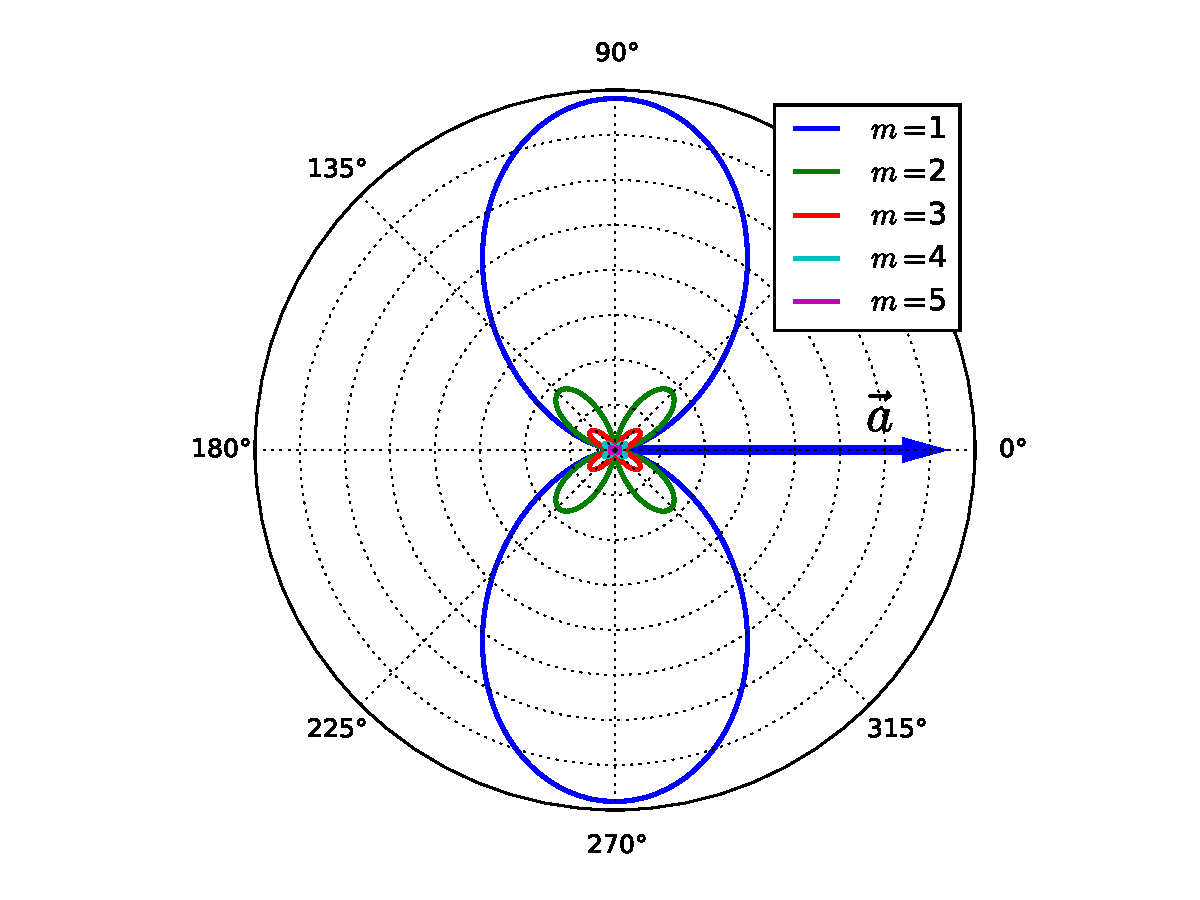
\psfig{file=fig/fig-mas.pdf,height=5cm,angle=0}}
 \caption{L'obulo de radiaci'on para $m=1,\dots,5$, $\beta=0,5$.}
\label{TER2}
\end{figure}
\begin{figure}[ht]
\centerline{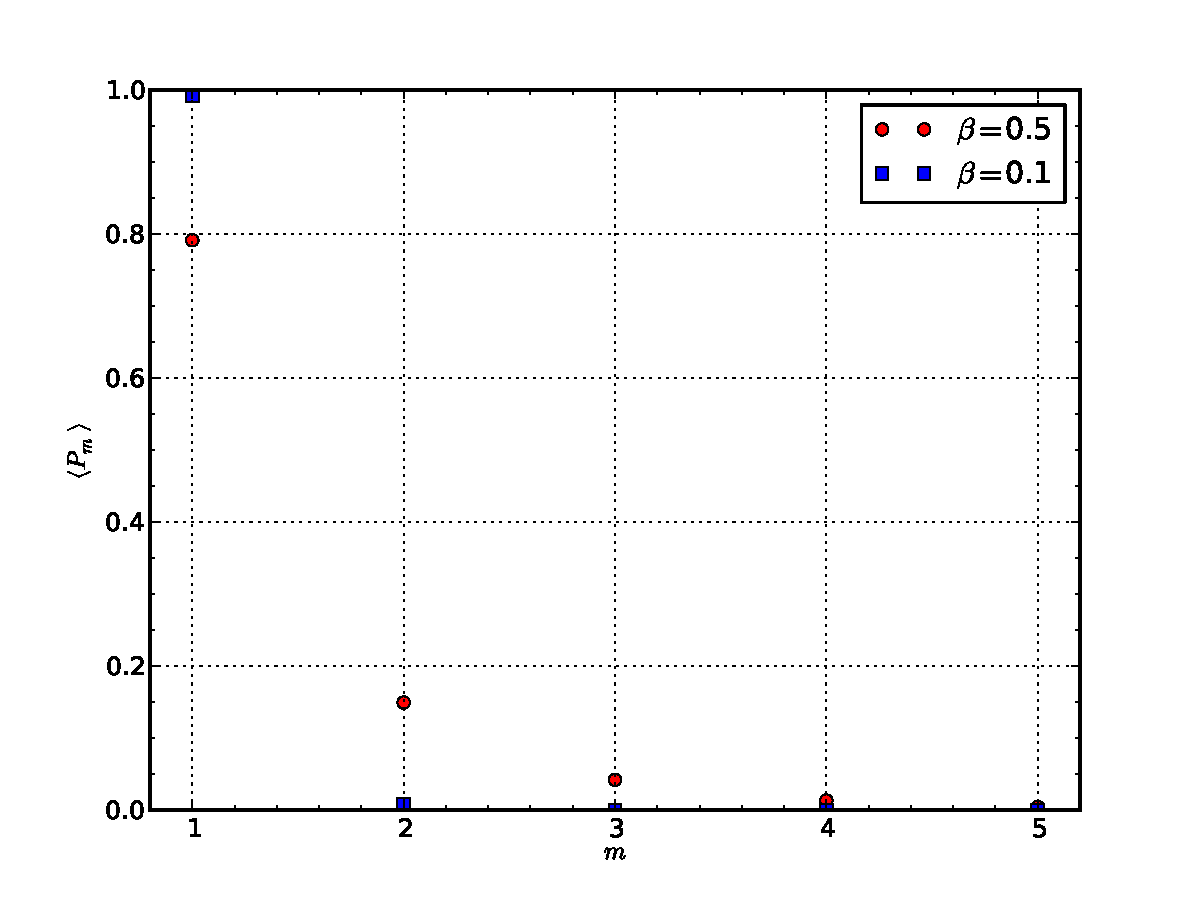
\psfig{file=fig/fig-mas-potencia-total-comparacion.pdf,height=5cm,angle=0}}
 \caption{Potencia promedio radiada para $m=1,\dots,5$, con par'ametros de velocidad $\beta=0,5$ y  $\beta=0,1$, normalizadas respecto a la potencia total.}
\label{TER3}
\end{figure}
Podemos comprobar que \textit{la mayor cantidad de energ'ia se irradia en la
frecuencia fundamental} $\omega_0$ (es decir, para $m=1$), mientras que los
arm'onicos superiores son en general suprimidos. Para movimientos
no-relativistas ($\beta\ll 1$) s'olo la frecuencia fundamental rad'ia
significativamente.

 En el l'imite no relativista, $\beta\ll 1$, podemos usar\footnote{Ver \cite{GR00}, p'agina 908, expresi'on 8.440, o \cite{AW01} p'agina 670, expresi'on (11.5).}
\begin{equation*}
J_{n}(x)\approx \frac{x^n}{2^nn!}, \qquad |x|\ll 1.
\end{equation*}
Por lo tanto, en este l'imite
\begin{equation}
\left\langle \frac{dP_{m}}{d\Omega}\right\rangle
\approx  \frac{\mu c}{8\pi^2}\left[\frac{q\omega_0}{(m-1)!}\left(\frac{a\omega_0m}{2c}\cos\theta\right)^{m}\tan\theta\right]^2.
\end{equation}
Adem'as, de aqu'i obtenemos
\begin{equation}
\frac{\left\langle \frac{dP_{m+1}}{d\Omega}\right\rangle}{\left\langle \frac{dP_{m}}{d\Omega}\right\rangle}\approx \left[\frac{a\omega_0}{2c}\cos\theta\right]^2=O(\beta^2),
\end{equation}
que muestra que la potencia radiada decrece en un factor del orden $\beta^2$ entre un arm'onico y el siguiente. Adem'as,
\begin{equation}
\left\langle \frac{dP_{1}}{d\Omega}\right\rangle
\approx  \frac{q^2\mu a^2\omega_0^4}{32\pi^2 c}\sen^2\theta.
\end{equation}

 Integrando con respecto al 'angulo s'olido obtenemos la potencia total promedio:
\begin{eqnarray}
\left\langle P_{1}\right\rangle&=& \int \left\langle\frac{dP_{1}}{d\Omega}\right\rangle\,d\Omega\\
&\approx &\frac{q^2\mu a^2\omega_0^4}{32\pi^2c}\,2\pi\int_{0}^{\pi
}\sin ^{3}\theta\, d\theta   \\
&\approx &\frac{q^2\mu a^2\omega_0^4}{16\pi c}\,\frac{4}{3}  \\
&\approx &\frac{q^2\mu a^2\omega_0^4}{12\pi c}.
\end{eqnarray}

Note la consistencia de este resultado con la f'ormula de Larmor (\ref{R-larmor}), ya que en este caso $\left\langle\vec{a}^2\right\rangle=\left\langle a^2\omega_0^4\cos^2(\omega_0t)\right\rangle=a^2\omega_0^4/2$.


\section{Dipolo de Hertz (dipolo el'ectrico ideal)}

En 1886 Hertz\footnote{Heinrich Rudolf Hertz (1857-1894): f'isico alem'an. Ver \url{http://es.wikipedia.org/wiki/Heinrich_Rudolf_Hertz}.} desarroll'o la primera \textit{antena dipolar} con la que realiz'o experimentos de emisi'on y recepci'on de \textit{ondas de radio} (``ondas hertzianas''). El modelo m'as sencillo de una antena dipolar es el de un \textit{dipolo el'ectrico con momento dipolar que cambia en el tiempo}.

Consideraremos entonces el modelo idealizado de un dipolo el'ectrico, formado por dos cargas $q_1=q$ y $q_2=-q$ situadas en las posiciones
\begin{equation}
 \vec{z}_1(t)=\frac{1}{2}\vec{d}(t), \qquad \vec{z}_2(t)=-\frac{1}{2}\vec{d}(t).
\end{equation}
El momento dipolar el'ectrico del sistema es dado por
\begin{equation}
 \vec{p}(t)=q\vec{d}(t).
\end{equation}
En un instante y una posici'on dada, el campo producido por este dipolo es la \textit{superposici'on del campo} correspondiente a cada carga. En particular, el potencial vectorial (siempre usando el gauge de Lorenz) es la suma de los potenciales vectoriales retardados, ver (\ref{potretq}b), de ambas cargas:
\begin{equation}
\vec{A}(\vec{x},t)=\frac{\mu c}{4\pi}\left[\left.\frac{q_1\vec{\beta}_1}{R_1(1-\hat{n}_1\cdot\vec{\beta}_1)}\right|_{{\rm ret}_1} +\left.\frac{q_2\vec{\beta}_2}{R_2(1-\hat{n}_2\cdot\vec{\beta}_2)}\right|_{{\rm ret}_2}\right].
\end{equation}
Note que las contribuciones de cada carga est'an evaluadas en el tiempo retardado correspondiente que, en general, \textit{es diferente}: $t'_1\neq t'_2$, ya que $\vec{z}_1(t)\neq\vec{z}_2(t)$.

Si las cargas se mueven a velocidades peque\~nas comparadas con la de la luz, $\beta_1\ll 1$, $\beta_2\ll 1$, podemos escribir
\begin{eqnarray}
\vec{A}(\vec{x},t)&\approx&\frac{\mu c}{4\pi}\left[\left.\frac{q_1\vec{\beta}_1}{R_1}(1+\hat{n}_1\cdot\vec{\beta}_1)\right|_{{\rm ret}_1} +\left.\frac{q_2\vec{\beta}_2}{R_2}(1+\hat{n}_2\cdot\vec{\beta}_2)\right|_{{\rm ret}_2}\right] \\
&=&\frac{q\mu c}{4\pi}\left[\left.\frac{\vec{\beta}_1}{R_1}\right|_{{\rm ret}_1} -\left.\frac{\vec{\beta}_2}{R_2}\right|_{{\rm ret}_2}\right] +O(\beta^2).
\end{eqnarray}
En el l'imite de ``dipolo ideal'' $d\to 0$ ($\vec{z}_1\to\vec{0}$, $\vec{z}_2\to\vec{0}$), tenemos que
\begin{equation}
 \vec{R}_1\to\vec{R}_2\to\vec{r}, \qquad \hat{n}_1\to\hat{n}_2\to\hat{r}, \qquad  t'_1=t'_2\to t-\frac{r}{c},
\end{equation}
y por lo tanto,
\begin{equation}
 \vec{A}(\vec{x},t)=\frac{q\mu c}{4\pi}\frac{1}{r}\left.(\vec{\beta}_1-\vec{\beta}_2)\right|_{t-\frac{r}{c}}.
\end{equation}
Podemos escribir este resultado en t'erminos de la variaci'on temporal del momento dipolar el'ectrico del sistema, ya que
\begin{equation}
q\left[\vec{\beta}_1(t)-\vec{\beta}_2(t)\right]=\frac{q}{c}\left[\dot{\vec{z}}_1(t)-\dot{\vec{z}}_2(t)\right]=\frac{q}{c}\dot{\vec{d}}(t)=\frac{\dot{\vec{p}}(t)}{c}.
\end{equation}
Entonces, para un dipolo ideal no-relativista, obtenemos
\begin{equation}
\boxed{\vec{A}(\vec{x},t)=\frac{\mu}{4\pi}\frac{\dot{\vec{p}}(t-{r}/{c})}{r}.} \label{Adipid}
\end{equation}
Podemos calcular el potencial escalar en forma an'aloga, es decir, a partir de la superposici'on de los potenciales retardados de las cargas que constituyen el dipolo. Alternativamente, podemos usar el hecho que los potenciales retardados fueron calculados usando el gauge de Lorenz. En efecto, usando \eqref{gLorenz} podemos calcular $\phi$ en t'erminos del potencial vectorial $\vec{A}$:
\begin{eqnarray}
\phi(\vec{x},t)&=&\phi(\vec{x},t_0)-c^2\int_{t_0}^t(\vec{\nabla}\cdot\vec{A})(\vec{x},\bar{t})\,d\bar{t} \\
&=&\phi(\vec{x},t_0)-\frac{\mu c^2}{4\pi} \vec{\nabla}\cdot\left[\frac{1}{r}\int_{t_0}^t\dot{\vec{p}}(\bar{t}-{r}/{c})\,d\bar{t}\right] \\
&=&\phi(\vec{x},t_0)-\frac{\mu c^2}{4\pi} \vec{\nabla}\cdot\left[\frac{1}{r}\left[\vec{p}(t-{r}/{c})-\vec{p}(t_0-{r}/{c})\right]\right] \\
&=&\phi(\vec{x},t_0)+\frac{1}{4\pi\varepsilon}\left[\frac{1}{r^2}\,\hat{r}\cdot\vec{p}(t-{r}/{c})+\frac{1}{cr}\hat{r}\cdot\dot{\vec{p}}(t-{r}/{c})\right] \nonumber\\
&& -\frac{1}{4\pi\varepsilon}\left[\frac{1}{r^2}\,\hat{r}\cdot\vec{p}(t_0-{r}/{c})+\frac{1}{cr}\hat{r}\cdot\dot{\vec{p}}(t_0-{r}/{c})\right] \\
&=& g(\vec{x},t)+\frac{1}{4\pi\varepsilon}\left[\frac{1}{r^2}\,\hat{r}\cdot\vec{p}(t-{r}/{c})+\frac{1}{cr}\hat{r}\cdot\dot{\vec{p}}(t-{r}/{c})\right] .
\end{eqnarray}
La funci'on $g(\vec{x},t)$ puede elegirse como nula imponiendo la condici'on que $\phi(\vec{x},t)$ se anule en el l'imite $\vec{p}\to\vec{0}$. Con esto, obtenemos 
\begin{equation}
\boxed{\phi(\vec{x},t)=\frac{1}{4\pi\varepsilon}\left[\frac{\hat{r}\cdot\vec{p}}{r^2}+\frac{\hat{r}\cdot\dot{\vec{p}}}{cr}\right]_{t-{r}/{c}}.} \label{phidipid}
\end{equation}
Vemos de este resultado que es posible diferenciar dos regiones del espacio, determinados por cu'al de los dos t'erminos que compone el potencial escalar ser'a predominante:

\paragraph{La \textit{zona cercana}} (near zone) se define como la zona en que
\begin{equation}
\phi(\vec{x},t)\approx\frac{1}{4\pi\varepsilon}\left.\frac{\hat{r}\cdot\vec{p}}{r^2}\right|_{\rm ret},
\end{equation}
es decir, en que \textit{el campo tiene la misma forma que en el caso est'atico}. M'as detalladamente, como el potencial tiene, cuando se expresa en t'erminos del momento dipolar, la misma forma funcional que en el caso est'atico, pero ahora con $\vec{p}=\vec{p}(t)$, se dice que el campo es \textit{cuasi-est'atico}. De la expresi'on \eqref{phidipid} vemos que esto ocurre para distancias $r$ tales que
\begin{equation}
|\dot{p}|r\ll c|p|.
\end{equation}

\paragraph{La \textit{zona lejana o zona de radiaci'on}} (far zone), por otro lado, corresponde a distancias lejanas tales que $|\dot{p}|r\gg c|p|$, de modo que
\begin{equation}
\phi(\vec{x},t)\approx\frac{1}{4\pi\varepsilon}\left.\frac{\hat{r}\cdot\dot{\vec{p}}}{cr}\right|_{\rm ret}.
\end{equation}

Por ejemplo, para un dipolo variando arm'onicamente, $\vec{p}(t)=\vec{p}_0\cos(\omega t)$, tenemos que la zona cercana est'a definida por $r\ll c/\omega=1/k=\lambda/2\pi$. En otras palabras, \textbf{las zonas cercana y lejana est'an definidas respecto de la distancia determinada por la longitud de onda de la radiaci'on emitida}.

Derivando los potenciales (\ref{Adipid}) y (\ref{phidipid}) obtenemos los campos el'ectrico y magn'etico correspondientes:
\begin{equation}
 \boxed{\vec{E}=\frac{1}{4\pi\varepsilon}\left[\frac{(\ddot{\vec{p}}\cdot\hat{r})\hat{r}-\ddot{\vec{p}}}{c^2r}+\frac{3(\dot{\vec{p}}\cdot\hat{r})\hat{r}-\dot{\vec{p}}}{cr^2}+\frac{3(\vec{p}\cdot\hat{r})\hat{r}-\vec{p}}{r^3}\right]_{\rm ret},}
\end{equation}
\begin{equation}
 \boxed{\vec{B}=\frac{\mu}{4\pi}\left[\frac{\ddot{\vec{p}}\times\hat{r}}{cr}+\frac{\dot{\vec{p}}\times\hat{r}}{r^2}\right]_{\rm ret}.}
\end{equation}
En la \textit{zona cercana}, los campos est'an dominados por las siguientes contribuciones:
\begin{equation}
 \vec{E}\approx\frac{1}{4\pi\varepsilon}\frac{3(\vec{p}\cdot\hat{r})\hat{r}-\vec{p}}{r^3},
\qquad
 \vec{B}\approx\frac{\mu}{4\pi}\frac{\dot{\vec{p}}\times\hat{r}}{r^2}.
\end{equation}
Por otro lado, en la \textit{zona lejana}, o \textit{zona de radiaci'on}, los campos est'an dominados por los t'erminos que decaen con $1/r$:
\begin{equation}
 \vec{E}\approx\vec{E}_{\rm rad}=\frac{1}{4\pi\varepsilon}\frac{(\ddot{\vec{p}}\cdot\hat{r})\hat{r}-\ddot{\vec{p}}}{c^2r}=\frac{1}{4\pi\varepsilon}\frac{(\ddot{\vec{p}}\times\hat{r})\times\hat{r}}{c^2r}, \qquad
 \vec{B}\approx \vec{B}_{\rm rad}=\frac{\mu}{4\pi}\frac{\ddot{\vec{p}}\times\hat{r}}{cr}.
\end{equation}
Notamos que estos campos satisfacen
\begin{equation}
 \vec{E}_{\rm rad}\cdot\hat{r}=0,\qquad  \vec{B}_{\rm rad}\cdot\hat{r}=0,\qquad \vec{B}_{\rm rad}=\frac{1}{c}\hat{r}\times\vec{E}_{\rm rad}, \qquad \vec{E}_{\rm rad}=c\vec{B}_{\rm rad}\times\hat{r},
\end{equation}
de modo que la parte radiativa del vector de Poynting es dada por
\begin{equation}
\vec{S}=\frac{1}{\mu c}\vec{E}\times(\hat{r}\times\vec{E}) 
=\frac{1}{\mu c}\vec{E}^2\,\hat{r}= \frac{\mu}{16\pi^2 c}\left|\frac{(\ddot{\vec{p}}\times\hat{r})\times\hat{r}}{r}\right|^2\hat{r} 
=\frac{\mu}{16\pi^2 c}\frac{\ddot{\vec{p}}{\,}^2}{r^2}\sen^2\theta\,\hat{r},
\end{equation}
donde $\theta$ es el 'angulo entre $\ddot{\vec{p}}$ y $\hat{r}$ (que, en general, depende del tiempo). La potencia radiada por el dipolo por unidad de 'angulo s'olido es entonces 
\begin{equation}
\boxed{\frac{dP}{d\Omega}%=r^2\vec{S}\cdot \hat{r}
=\frac{\mu}{16\pi^2 c}\left.{\ddot{\vec{p}}{\,}^2}\sen^2\theta\right|_{\rm ret}.}
\end{equation}
\begin{figure}[H]
\centerline{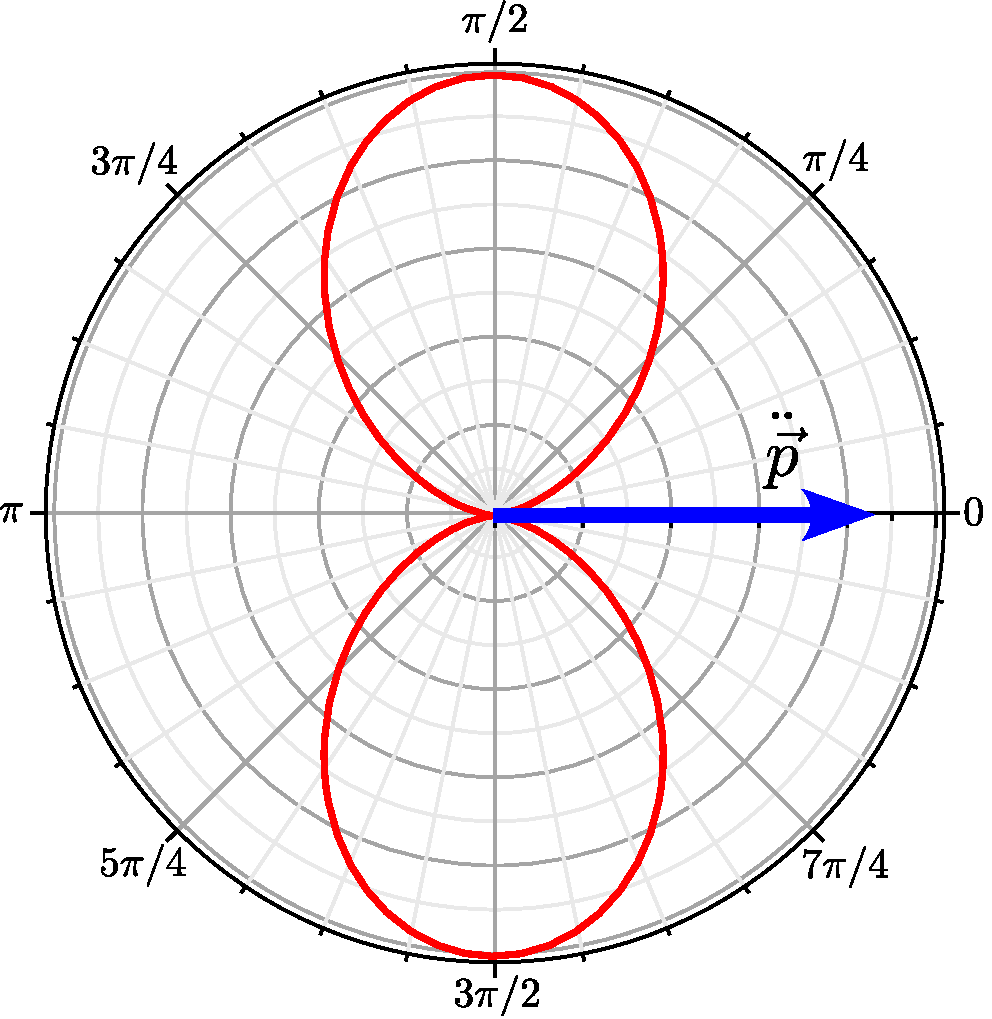
\psfig{file=fig/fig-dipolo.pdf,height=5cm,angle=0}}
 \caption{L'obulo de radiaci'on de un dipolo ideal.}
\label{fig-dipolo}
\end{figure}
Finalmente, la potencia (instant'anea) total radiada adopta una forma an'aloga a aquella dada por la f'ormula de Larmor, ver \eqref{R-larmor}:
\begin{equation}\label{PotdH}
\boxed{P=\frac{\mu}{6\pi c}\left.\ddot{\vec{p}}{\,}^2\right|_{\rm ret}.}
\end{equation}

Para un dipolo variando \textit{arm'onicamente} en el tiempo con frecuencia angular $\omega$, de modo que $\ddot{\vec{p}}(t)=-\omega^2\vec{p}(t)$, la \textit{potencia promedio} puede escribirse como:
\begin{equation}
\left\langle P\right\rangle
=\frac{\mu}{6\pi c}\left\langle\left.\ddot{\vec{p}}{\,}^2\right|_{\rm ret}\right\rangle 
=\frac{\mu}{6\pi c}\omega^4\left\langle\left.\vec{p}^2\right|_{\rm ret}\right\rangle
=\frac{\mu}{12\pi c}\omega^4 p_0^2,
%=\frac{(2\pi)^3\mu}{6c}\frac{p_0^2}{\lambda^4},
\end{equation}
con $p_0^2:=2\left\langle \vec{p}{\,}^2(t)\right\rangle$.


\section{Radiaci'on de una peque\~na espira de corriente}

Consideremos un peque\~no circuito (una espira) circular, de radio $a$, por el cual fluye una corriente $I(t)$. Consideraremos adem'as que en todo momento  el cable es el'ectricamente neutro y que la corriente que circula por 'el es uniforme. Entonces, $\rho=0$ y por lo tanto podemos considerar que $\phi=0$.

El potencial vectorial es dado por la expresi'on general (\ref{potret}b). Como en este caso la distribuci'on de corriente es unidimensional, podemos reemplazar $\vec{J}\,dV'$ por $I\,d\vec{\ell} '$, de modo que
\begin{equation}
 \vec{A}(\vec{x},t)=\frac{\mu}{4\pi}\oint \frac{I(t_{\rm ret})}{R}d\vec{\ell} ' , \label{Aloop1}
\end{equation}
con $R=|\vec{x}-\vec{x}'|$ y $t_{\rm ret}=t-R/c$.

En analog'ia con lo discutido en la secci'on anterior, consideraremos el caso de un \textit{dipolo magn'etico ideal}, que corresponde al l'imite en que $a\to 0$, pero $\mu=AI=\pi a^2I$ tiende a un valor finito.

Sobre la circunferencia de la espira tenemos que $\vec{x}'=a\hat{r}'$. Adicionalmente, expandiremos (\ref{Aloop1}) en potencias de $a/r\ll 1$.  Comenzamos expandiendo $R$:
\begin{eqnarray}
 R&=&r\left|\hat{r}-\frac{a\hat{r}'}{r}\right| \\
&=&r\left(1-\frac{a}{r}\hat{r}\cdot\hat{r}'+O(a^2)\right) \\
&=& r-a\hat{r}\cdot\hat{r}'+O(a^2).
\end{eqnarray}
Como consecuencia de esto, obtenemos
\begin{equation}
 \frac{1}{R}=\frac{1}{r}+\frac{a}{r^2}\hat{r}\cdot\hat{r}'+O(a^2),
\end{equation}
y adem'as,
\begin{equation}
 t_{\rm ret}=t-\frac{r}{c}+\frac{a}{c}\hat{r}\cdot\hat{r}'+O(a^2).
\end{equation}
Expandiremos ahora la expresi'on $I(t_{\rm ret})$:
\begin{eqnarray}
 I(t_{\rm ret})
&=&I\left(t-\frac{r}{c}+\frac{a}{c}\hat{r}\cdot\hat{r}'+O(a^2)\right) \\
&=&I\left(t-\frac{r}{c}\right)+\dot{I}\left(t-\frac{r}{c}\right)\left(\frac{a}{c}\hat{r}\cdot\hat{r}'\right)+O(a^2).
\end{eqnarray}
De esta forma, podemos escribir que
\begin{eqnarray}
\frac{I(t_{\rm ret})}{R}
&=&\left[\frac{1}{r}+\frac{a}{r^2}\hat{r}\cdot\hat{r}'+O(a^2)\right]\left[I\left(t-\frac{r}{c}\right)+\dot{I}\left(t-\frac{r}{c}\right)\left(\frac{a}{c}\hat{r}\cdot\hat{r}'\right)+O(a^2)\right]\\
&=&\frac{I}{r}+\frac{a\dot{I}}{cr}(\hat{r}\cdot\hat{r}')+\frac{aI}{r^2}(\hat{r}\cdot\hat{r}')
+O(a^2)\\
&=&\frac{I}{r}+\frac{a\dot{I}}{cr}(\hat{r}\cdot\hat{r}')+\frac{aI}{r^2}(\hat{r}\cdot\hat{r}')+O(a^2).
\end{eqnarray}
Note que para simplificar la notaci'on hemos omitido explicitar que las funciones $I$ y $\dot{I}$ est'an evaluadas en el tiempo $t':=t-r/c$. Al introducir esta expansi'on en (\ref{Aloop1}) obtenemos:
\begin{eqnarray}
 \vec{A}(\vec{x},t)&=&\frac{\mu}{4\pi r}\left[I\oint d\vec{\ell}'
+\frac{a\dot{I}}{c}\oint(\hat{r}\cdot\hat{r}')d\vec{\ell}'+\frac{aI}{r}\oint(\hat{r}\cdot\hat{r}')d\vec{\ell}'+O(a^2)\right]  \\
&=&\frac{\mu}{4\pi r}\left[Ia\oint d\hat{r}'
+\frac{a^2\dot{I}}{c}\oint(\hat{r}\cdot\hat{r}')d\hat{r}'+\frac{a^2I}{r}\oint(\hat{r}\cdot\hat{r}')d\hat{r}'\right] +O(a^3).
\end{eqnarray}
Pero $\oint d\hat{r}'=\vec{0}$ sobre toda curva cerrada. Adem'as un simple c'alculo muestra que para cualquier curva cerrada plana (como nuestra espira) se satisface 
\begin{equation}
\oint(\hat{r}\cdot\hat{r}')d\hat{r}'=\pi(\hat{z}\times\hat{r}) .
\end{equation}
Con esto, e introduciendo el \textit{momento magn'etico} de la espira, $\vec{\mu}=\pi a^2I\hat{z}$, obtenemos
\begin{equation}
 \boxed{\vec{A}(\vec{x},t)=\frac{\mu}{4\pi}\left[\frac{\vec{\mu}\times\hat{r}}{r^2}+\frac{\dot{\vec{\mu}}\times\hat{r}}{cr}\right]_{\rm ret}.}
\end{equation}

Calculamos ahora los campos el'ectrico y magn'etico a partir de los potenciales. Obtenemos que
\begin{equation}
 \boxed{\vec{E}(\vec{x},t)=\frac{\mu}{4\pi}\left[\frac{\hat{r}\times\dot{\vec{\mu}}}{r^2}+\frac{\hat{r}\times\ddot{\vec{\mu}}}{cr}\right]_{\rm ret},}
\end{equation}
\begin{equation}
\boxed{ \vec{B}(\vec{x},t)=\frac{\mu}{4\pi}\left[\frac{3(\hat{r}\cdot\vec{\mu})\hat{r}-\vec{\mu}}{r^3}+\frac{3(\hat{r}\cdot\dot{\vec{\mu}})\hat{r}-\dot{\vec{\mu}}}{cr^2}+\frac{(\hat{r}\cdot\ddot{\vec{\mu}})\hat{r}-\ddot{\vec{\mu}}}{c^2r}\right]_{\rm ret}.}
\end{equation}
Tal como hemos visto en los casos anteriores, las componentes radiativas son aquellas que decaen con $1/r$, es decir,
\begin{equation}
 \boxed{\vec{E}_{\rm rad}(\vec{x},t)
=\frac{\mu}{4\pi c}\frac{\hat{r}\times\ddot{\vec{\mu}}}{r},} \qquad
 \boxed{\vec{B}_{\rm rad}(\vec{x},t)=\frac{\mu}{4\pi c^2}\frac{(\hat{r}\cdot\ddot{\vec{\mu}})\hat{r}-\ddot{\vec{\mu}}}{r}.}
\end{equation}

Como es directo de verificar, estos campos satisfacen nuevamente las relaciones:
\begin{equation}
\vec{E}_{\rm rad}\cdot\hat{r}=0, \qquad \vec{B}_{\rm rad}\cdot\hat{r}=0, \qquad \vec{B}_{\rm rad}=\frac{1}{c}\hat{r}\times\vec{E}_{\rm rad}, \quad \vec{E}_{\rm rad}=c\vec{B}_{\rm rad}\times\hat{r},
\end{equation}
tal como es t'ipico de un campo de radiaci'on. Como consecuencia, el vector de Poynting adopta la forma $\vec{S}=(1/\mu c)\vec{E}_{\rm rad}^2\hat{r}$, de modo que la energ'ia se propaga en la direcci'on del vector $\hat{r}$. La potencia por unidad de 'angulo s'olido radiada por la peque\~na espira de corriente es entonces
\begin{equation}
\boxed{\frac{dP}{d\Omega}(\hat{r},t)=\frac{\mu}{16\pi^2 c^3}\ddot{\vec{\mu}}{\,}^2\sen^2\theta ,}
\end{equation}
donde $\theta$ es ahora el 'angulo entre $\ddot{\vec{\mu}}$ y $\hat{r}$. La potencia total radiada es entonces

\begin{equation}\label{Pdipmag}
\boxed{P(t)=\frac{\mu}{6\pi}\frac{\ddot{\vec{\mu}}{\,}^2}{c^3}.}
\end{equation}

\section{Resistencia de radiaci'on}

En un circuito el'ectrico con una fuente y una resistencia, la potencia instant'anea disipada (en calor) por la resistencia es dada por $P(t)=RI^2(t)$. Para el caso de corrientes peri'odicas, la potencia disipada promedio es entonces dada por $\left\langle P\right\rangle=R\left\langle I^2\right\rangle$.
An'alogamente, en el caso de un sistema de cargas y corrientes que rad'ia una potencia promedio $\left\langle P_{\rm rad}\right\rangle$ y es alimentada por una corriente $I(t)$, se define la \textit{resistencia de radiaci'on} $R_{\rm rad}$ por
\begin{equation}
R_{\rm rad}:=\frac{\left\langle P_{\rm rad}\right\rangle}{\left\langle I^2\right\rangle}.
\end{equation}

\subsection{Resistencia de radiaci'on de un dipolo de Hertz}\label{sec:RRdH}
Consideremos el caso en que el dipolo est'a constituido por un (peque\~no) condensador de placas paralelas. Entonces el momento dipolar del sistema es dado por $p(t)=Q(t)d$, donde $Q(t)$ es la magnitud de la carga almacenada en las placas en el instante $t$ y $d$ es la distancia entre las placas. Entonces $\dot{p}(t)=\dot{Q}(t)d=I(t)d$, donde $I(t)$ es la corriente que alimenta al condensador. Usando esta expresi'on, podemos evaluar la potencia \eqref{PotdH} radiada por el dipolo, obteniendo
%\begin{equation}
%\left\langle P_{\rm rad}\right\rangle=\frac{2}{3}\frac{\langle \dot{I}^2\rangle d^2}{c^3}
%\end{equation}
%o, en unidades S.I.,
\begin{equation}
\left\langle P_{\rm rad}\right\rangle=\frac{\mu}{6\pi c}{\langle\dot{I}^2\rangle d^2}.
\end{equation}
Si la corriente que alimenta el sistema es peri'odica con frecuencia angular $\omega$ entonces $\langle\dot{I}^2\rangle=\omega^2\langle I^2\rangle$ y por lo tanto
\begin{equation}
\left\langle P_{\rm rad}\right\rangle=\frac{\mu}{6\pi c}{\langle I^2\rangle \omega^2d^2}.
\end{equation}
La resistencia de radiaci'on en este caso es dada por
\begin{equation}\label{Rradp}
R_{\rm rad}=\frac{\mu}{6\pi c}{\omega^2d^2}
=\frac{2\pi}{3}\mu c\left(\frac{d}{\lambda}\right)^2
=\frac{2\pi}{3}Z_0\left(\frac{d}{\lambda}\right)^2,
\end{equation}
donde hemos introducido la constante $Z:=\mu c=1/\varepsilon c=\sqrt{\mu/\varepsilon}$, que en el vac'io asume el valor $Z_0=119,9169832\pi\,[\Omega]\approx 377\,[\Omega]$. En este caso, $Z_0$ es llamada la \textit{impedancia del vac'io}, o \textit{impedancia del espacio libre}.

\subsection{Resistencia de radiaci'on de una peque\~na espira}
Consideramos una peque\~na espira circular, de radio $a$, que es alimentada por una fuente que suministra una diferencia de potencial variable, de modo que la corriente que circula por la espira es dada por $I(t)$. En este caso, el momento magn'etico del sistema tiene m'odulo $\mu(t)=\pi a^2I(t)$. Suponiendo que la corriente que circula por la espira var'ia arm'onicamente en el tiempo, con frecuencia angular $\omega$, y que $a\ll c/\omega$, podemos modelar la radiaci'on emitida como aquella producida por un dipolo magn'etico ideal. Bajo estas condiciones, la expresi'on (\ref{Pdipmag}) nos permite escribir
\begin{equation}
\left\langle P_{\rm rad}\right\rangle=\frac{\mu}{6\pi c^3}{\left\langle \ddot{\mu}^2\right\rangle}=\frac{\pi\mu}{6c^3}{a^4}\left\langle \ddot{I}^ 2\right\rangle .
\end{equation}
%o, en unidades del Sistema Internacional,
%\begin{equation}
%\left\langle P_{\rm rad}\right\rangle=\frac{\pi}{6\varepsilon_0}\frac{a^4}{c^5}\left\langle \ddot{I}^ 2\right\rangle.
%\end{equation}
Como suponemos que la corriente var'ia arm'onicamente en el tiempo, tendremos que $\langle\ddot{I}^ 2\rangle=\omega^4\langle I^ 2\rangle$ y, por lo tanto, la resistencia de radiaci'on resulta ser
\begin{equation}
R_{\rm rad}=\frac{\pi\mu}{6c^3}{a^4\omega^4}
=\frac{8\pi^5}{3}Z\left(\frac{a}{\lambda}\right)^4.
\end{equation}
Evaluando esta expresi'on en el caso del vac'io, encontramos
\begin{equation}\label{Rradmu}
R_{\rm rad}\approx 6,4\times 10^{5}\left(\frac{a}{\lambda}\right)^4 [\Omega].
\end{equation}

Consideremos finalmente que con una misma corriente se alimenta el condensador discutido en la secci'on \ref{sec:RRdH} y, alternativamente, la espira que acabamos de analizar. Si ambos sistemas son \textit{aproximadamente del mismo tama\~no} ($d\approx a$) podemos escribir, usando los resultados (\ref{Rradp}) y (\ref{Rradmu}), 
\begin{equation}
\frac{R_{\rm rad}^{\vec\mu}}{R_{\rm rad}^{\vec{p}}}\approx 4\pi^4\left(\frac{a}{\lambda}\right)^2=\pi^2\left(\frac{2\pi a}{\lambda}\right)^2\approx 10\left(\frac{2\pi a}{\lambda}\right)^2.
\end{equation}
Por lo tanto, como hemos supuesto que $a\ll\lambda/2\pi$, encontramos que  $R_{\rm rad}^{\vec\mu}\ll R_{\rm rad}^{\vec{p}}$. En este sentido un peque\~no condensador rad'ia m'as ``eficientemente'' que una espira de similar tama\~no, alimentada con la misma corriente alterna.


\section{Campos radiativos de una distribuci'on general de carga y corriente}

Aqu'i nos concentraremos en determinar s'olo las \textit{componentes radiativas} de los campos generados \textit{por una distribuci'on general de carga y corriente}. Estos campos corresponden a los t'erminos de $\vec{E}$ y $\vec{B}$ que decaen como $1/r$, ya que s'olo 'estos contribuyen a la potencia radiada. En t'erminos de los potenciales electromagn'eticos, es tambi'en suficiente calcular los t'erminos que decaen con $1/r$.

En este caso general, los potenciales retardados son dados por las expresiones (\ref{potret}). Ya que estamos interesados en el \textit{campo de radiaci'on}, muy lejos de la fuente, podemos realizar una expansi'on en potencias de $\vec{x}'/r\ll 1$ de las cantidades involucradas en (\ref{potret}):
\begin{eqnarray}
 R&=&r\left|\hat{r}-\frac{\vec{x}'}{r}\right| \\
&=&r\left(1-\frac{\hat{r}\cdot\vec{x}'}{r}+O(r^{-2})\right) \\
&=& r-\hat{r}\cdot\vec{x}'+O(r^{-1}),
\end{eqnarray}
\begin{equation}
 \frac{1}{R}=\frac{1}{r}+O(r^{-2}),
\end{equation}
y
\begin{equation}
 t_{\rm ret}=t-\frac{r}{c}+\frac{\hat{r}\cdot\vec{x}'}{c}+O(r^{-1}).
\end{equation}
Para calcular los campos incluyendo t'erminos hasta orden $1/r$ es suficiente expandir $\rho(\vec{x}',t_{\rm ret})$ y $\vec{J}(\vec{x}',t_{\rm ret})$ a orden 0 en potencias de $1/r$, es decir,
\begin{equation}
 \rho(\vec{x}',t_{\rm ret})=\rho(\vec{x}',t-\frac{r}{c}+\frac{\hat{r}\cdot\vec{x}'}{c})+O(r^{-1}),
\end{equation}
de modo que
\begin{equation}
 \frac{\rho(\vec{x}',t_{\rm ret})}{R}=\frac{1}{r}\rho(\vec{x}',t-\frac{r}{c}+\frac{\hat{r}\cdot\vec{x}'}{c})+O(r^{-2}),
\end{equation}
y, similarmente,
\begin{equation}
 \frac{\vec{J}(\vec{x}',t_{\rm ret})}{R}=\frac{1}{r}\vec{J}(\vec{x}',t-\frac{r}{c}+\frac{\hat{r}\cdot\vec{x}'}{c})+O(r^{-2}).
\end{equation}
Estas expansiones son v'alidas para $r\gg d$, donde $d$ es el (orden de magnitud del) tama\~no (lineal) de la distribuci'on de cargas y corrientes. Con ellas, las integrales generales (\ref{potret}) se reducen a
\begin{equation}
 \phi(\vec{x},t)=\frac{1}{4\pi\varepsilon}\frac{1}{r}\int\rho(\vec{x}',t-\frac{r}{c}+\frac{\hat{r}\cdot\vec{x}'}{c})\,dV'+O(r^{-2}),
\end{equation}
\begin{equation}
 \vec{A}(\vec{x},t)=\frac{\mu}{4\pi}\frac{1}{r}\int\vec{J}(\vec{x}',t-\frac{r}{c}+\frac{\hat{r}\cdot\vec{x}'}{c})\,dV'+O(r^{-2}).
\end{equation}
En otras palabras,
\begin{equation}
 \boxed{\phi_{\rm rad}(\vec{x},t)
=\frac{1}{4\pi\varepsilon}\frac{1}{r}\int\rho(\vec{x}',t-\frac{r}{c}+\frac{\hat{r}\cdot\vec{x}'}{c})\,dV',} \label{phirad}
\end{equation}
\begin{equation}
 \boxed{\vec{A}_{\rm rad}(\vec{x},t)
=\frac{\mu}{4\pi}\frac{1}{r}\int\vec{J}(\vec{x}',t-\frac{r}{c}+\frac{\hat{r}\cdot\vec{x}'}{c})\,dV'.} \label{Arad}
\end{equation}

\subsection{Expansi'on multipolar}\label{sec:emr}

Podemos expresar \eqref{phirad} y \eqref{Arad} como una suma de t'erminos proporcionales a los \textit{momentos multipolares el'ectricos y magn'eticos de la distribuci'on de cargas y corrientes} que es fuente del campo. Para esto, expandimos los integrandos de \eqref{phirad} y \eqref{Arad} en potencias de $(\hat{r}\cdot\vec{x}')/c$. Por ejemplo,
\begin{eqnarray}
 \rho(\vec{x}',t'+\frac{\hat{r}\cdot\vec{x}'}{c})&=&\rho(\vec{x}',t')+\left(\frac{\hat{r}\cdot\vec{x}'}{c}\right)\dot\rho(\vec{x}',t')+\frac{1}{2}\left(\frac{\hat{r}\cdot\vec{x}'}{c}\right)^2\ddot\rho(\vec{x}',t') \nonumber\\
 &&+\cdots+\frac{1}{n!}\left(\frac{\hat{r}\cdot\vec{x}'}{c}\right)^n\stackrel{(n)}{\rho}\!\!\!(\vec{x}',t')+\cdots ,
\end{eqnarray}
donde hemos denotado $t':=t-r/c$ y $\stackrel{(n)}{\rho}:=\partial^n\rho/\partial t^n$ es la $n$-'esima derivada parcial de $\rho$ respecto al tiempo.

Esta expansi'on tendr'a t'erminos cada vez m'as peque\~nos, y por lo tanto su \textit{truncamiento} a 'ordenes cada vez mayores suministrar'a \textit{mejores aproximaciones} al resultado exacto, si se satisface (en cada punto de la distribuci'on) que
\begin{equation}
 |\rho|\gg \frac{|\dot{\rho}|d}{c}, \qquad  |\dot{\rho}|\gg \frac{|\ddot{\rho}|d}{c},
\end{equation}
etc., es decir, si
\begin{equation}
|\stackrel{(n)}{\rho}|\gg \frac{d}{c}\,|\stackrel{(n+1)}{\rho}|, \qquad n=0,1,2,\cdots .
\end{equation}
Si la fuente \textit{var'ia temporalmente en forma arm'onica}, por ejemplo si $\rho(\vec{x},t)=\rho_0(\vec{x})\cos(\omega t)$, entonces la condici'on anterior es equivalente (para todo $n$) a
\begin{equation}
d\ll\frac{c}{\omega}=\frac{\lambda}{2\pi},
\end{equation}
es decir, a que \textbf{el tama\~no (lineal) de la fuente sea mucho menor que la longitud de onda asociada a la frecuencia $\omega$}. Recuerde que siempre es posible \textit{descomponer $\rho$ en una superposici'on de oscilaciones arm'onicas}, v'ia an'alisis de Fourier.

Suponiendo que las condiciones anteriores se satisfacen, podemos escribir:
\begin{align}
\phi_{\rm rad}(\vec{x},t)
 &= \frac{1}{4\pi\varepsilon}\frac{1}{r}\left[  \int\rho\,dV'+\frac{\hat{r}_i}{c}\int\dot{\rho}x'_i\,dV'+\frac{1}{2}\frac{\hat{r}_i}{c}\frac{\hat{r}_j}{c}\int\ddot{\rho}x'_ix'_j\,dV'\right. \nonumber \\
 &\qquad\qquad\  \left.+\cdots +
\frac{1}{n!}\frac{\hat{r}_{j_1}}{c}\cdots\frac{\hat{r}_{j_n}}{c}\int\stackrel{(n)}{\rho}\!\!\!x'_{j_1}\cdots x'_{j_n}\,dV'+\cdots\right] \\
 &= \frac{1}{4\pi\varepsilon}\frac{1}{r}\left[  \int\rho\,dV'+\frac{\hat{r}_i}{c}\frac{d\ }{dt}\left(\int\rho x'_i\,dV'\right)+\frac{1}{2}\frac{\hat{r}_i}{c}\frac{\hat{r}_j}{c}\frac{d^2\ }{dt^2}\left(\int\rho x'_ix'_j\,dV'\right)\right. \nonumber \\
 &\qquad\qquad\ \left.+\cdots +
\frac{1}{n!}\frac{\hat{r}_{j_1}}{c}\cdots\frac{\hat{r}_{j_n}}{c}\frac{d^n\ }{dt^n}\left(\int\rho x'_{j_1}\cdots x'_{j_n}\,dV'\right) +\cdots\right] \\
 &= \frac{1}{4\pi\varepsilon}\frac{1}{r}\left[  Q+\frac{\hat{r}_i}{c}\frac{d\ }{dt}Q_i+\frac{1}{2}\frac{\hat{r}_i}{c}\frac{\hat{r}_j}{c}\frac{d^2\ }{dt^2}Q_{ij}\right. \nonumber \\
 &\qquad\qquad\ \left.+\cdots +\frac{1}{n!}\frac{\hat{r}_{j_1}}{c}\cdots\frac{\hat{r}_{j_n}}{c}\frac{d^n\ }{dt^n}Q_{j_1\cdots j_n} +\cdots\right] ,
\end{align}
donde
\begin{equation}
 Q_{j_1\cdots j_n}(t):=\int\rho(\vec{x}',t)\, x'_{j_1}\cdots x'_{j_n}\,dV'
\end{equation}
es el \textit{momento multipolar el'ectrico de orden} $n$. En resumen,
\begin{align}
 \phi_{\rm rad}(\vec{x},t) &= \frac{1}{4\pi\varepsilon}\frac{1}{r}\left[  Q(t')+\frac{\hat{r}_i}{c}\dot{Q}_i(t')+\frac{1}{2}\frac{\hat{r}_i}{c}\frac{\hat{r}_j}{c}\ddot{Q}_{ij}(t') \right.\nonumber\\
& \qquad\qquad\ \left.+\cdots +\frac{1}{n!}\frac{\hat{r}_{j_1}}{c}\cdots\frac{\hat{r}_{j_n}}{c}\stackrel{(n)}{Q}\!\!{}_{j_1\cdots j_n}(t') +\cdots\right] .  \label{emprad}
\end{align}
An'alogamente, para el potencial vectorial, tendremos la siguiente expansi'on
\begin{align}
A_i^{\rm rad}(\vec{x},t) &= \frac{\mu}{4\pi}\frac{1}{r}\left[  M_i(t')+\frac{\hat{r}_j}{c}\dot{M}_{ji}(t')+\frac{1}{2}\frac{\hat{r}_j}{c}\frac{\hat{r}_k}{c}\ddot{M}_{jki}(t')\right.\nonumber\\
& \qquad\qquad\ \left.+\cdots +\frac{1}{n!}\frac{\hat{r}_{j_1}}{c}\cdots\frac{\hat{r}_{j_n}}{c}\stackrel{(n)}{M}\!\!{}_{j_1\cdots j_ni}(t') +\cdots\right] , \label{emArad}
\end{align}
donde
\begin{equation}
 M_{j_1\cdots j_ni}(t):=\int x'_{j_1}\cdots x'_{j_n}J_i(\vec{x}',t)\,dV'
\end{equation}
denotan los \textit{momentos multipolares magn'eticos de orden} $n$ de la distribuci'on. Note que en (\ref{emprad}) y (\ref{emArad}) (las derivadas de) los momentos multipolares est'an evaluados en el tiempo retardado $t'=t-r/c$.

Calculamos ahora la componente radiativa del campo el'ectrico, es decir, aquella que decae con $1/r$ a grandes distancias. A partir de (\ref{emprad}) y (\ref{emArad}) encontramos que
\begin{align}
E_i^{\rm rad}(\vec{x},t) &= \frac{\mu c}{4\pi}\frac{1}{r}\left[\hat{r}_i\dot{Q}+\frac{1}{c}\left(\hat{r}_i\hat{r}_j\ddot{p}_j-\dot{M}_i\right)+\frac{1}{2c^2}\left(\hat{r}_i\hat{r}_j\hat{r}_k\dddot{Q}_{jk} -2\hat{r}_j\ddot{M}_{ji}\right)+\cdots\right.\nonumber\\
& \qquad\qquad \left.+\frac{1}{n!c^n}\hat{r}_{j_1}\cdots\hat{r}_{j_{n-1}}\left(\!\stackrel{(n+1)}{Q}\!\!\!\!\!{}_{j_1\cdots j_n}\hat{r}_{j_n}\hat{r}_i- n\stackrel{(n)}{M}\!\!{}_{j_1\cdots j_{n-1}i}\right)+\cdots\right]_{\rm ret}. \label{emErad}
\end{align}

Para un sistema de cargas y corrientes que est'e \textit{aislado el'ectricamente} la carga total del sistema permanece constante, de modo que $\dot{Q}=0$. Por otro lado, \textit{el momento monopolar magn'etico $M_i$ es proporcional a la variaci'on temporal del momento dipolar el'ectrico $p_i$}. En efecto, en el caso magnetost'atico se tiene que $M_i=0$, lo que puede ser demostrado considerando la integral $\oint_Sx_iJ_j\, dS_j$ en una superficie $S$ que encierre la distribuci'on de cargas y corrientes, pero sobre la cual $\vec{J}=\vec{0}$. Ver secci'on \ref{sec:emm}. En el caso no estacionario que ahora consideramos, tenemos que
\begin{eqnarray}
 0&=&\oint_Sx_iJ_j\, dS_j\\
&=&\int_V\partial_j(x_iJ_j)\,dV \\
&=&\int_VJ_i\,dV+\int_Vx_i(\partial_jJ_j)\,dV \\
&=&M_i-\int_Vx_i(\partial_t\rho)\,dV \\
&=&M_i-\frac{d\ }{dt}\int_Vx_i\rho\,dV \\
&=&M_i-\dot{p}_i,
\end{eqnarray}
donde hemos usado el teorema de Gauss y la ecuaci'on de continuidad. Por lo tanto,
\begin{equation}
 \vec{M}=\dot{\vec{p}}.
\end{equation}
An'alogamente, para el momento dipolar magn'etico podemos considerar la siguiente integral:
\begin{eqnarray}
 0&=&\oint_Sx_ix_jJ_k\, dS_k\\
&=&\int_V\partial_k(x_ix_jJ_k)\,dV \\
&=&\int_V(x_jJ_i+x_iJ_j)\,dV+\int_Vx_ix_j(\partial_kJ_k)\,dV \\
&=&\int_V(x_jJ_i+x_iJ_j)\,dV-\int_Vx_ix_j(\partial_t\rho)\,dV \\
&=&2M_{(ij)}-\dot{Q}_{ij}.
\end{eqnarray}
En otras palabras, \textit{la parte sim'etrica de $M_{ij}$ es igual a la variaci'on temporal del momento cuadrupolar el'ectrico}. Por otro lado, la parte antisim'etrica es, por definici'on, proporcional al \textit{(pesudo-)vector momento dipolar magn'etico} $\vec{\mu}$:
\begin{equation}
 M_{[ij]}=\epsilon_{ijk}\mu_k, \qquad \mu_k:=\frac{1}{2}\epsilon_{ijk}\int_Vx_jJ_k\,dV.
\end{equation}
En resumen,
\begin{equation}
 M_{ij}=\frac{1}{2}\dot{Q}_{ij}+\epsilon_{ijk}\mu_k.
\end{equation}
Con esto, podemos reescribir \eqref{emErad} como
\begin{equation}
\boxed{E_i^{\rm rad}(\vec{x},t)=\frac{\mu}{4\pi}\frac{1}{r}\left[\left(\hat{r}_i\hat{r}_j\ddot{p}_j-\ddot{p}_i\right)+\frac{1}{c}\epsilon_{ijk}\hat{r}_j\ddot{\mu}_k+\frac{1}{2c}\left(\hat{r}_i\hat{r}_j\hat{r}_k\dddot{Q}_{jk} -\hat{r}_j\dddot{Q}_{ji}\right)+\cdots\right]_{\rm ret} .} \label{emErad2}
\end{equation}
Vemos entonces que el primer t'ermino corresponde al campo de radiaci'on de un \textit{dipolo el'ectrico} (ideal), el segundo al de un \textit{dipolo magn'etico} (ideal). El tercero es la \textit{contribuci'on cuadrupolar el'ectrica}, etc.

Por otro lado, usando (\ref{emprad}) y (\ref{emArad}) puede verificarse que
\begin{equation}
 \vec{B}_{\rm rad}(\vec{x},t)=\frac{1}{c}\hat{r}\times\vec{E}_{\rm rad}(\vec{x},t), \quad  \vec{E}_{\rm rad}(\vec{x},t)=c\vec{B}_{\rm rad}(\vec{x},t)\times\hat{r}, \quad \vec{E}_{\rm rad}\times\vec{B}_{\rm rad}=\frac{1}{c}\left|\vec{E}_{\rm rad}\right|^2\hat{r},
\end{equation}
como es usual para un campo de radiaci'on. De aqu'i obtenemos, finalmente, una expansi'on para la \textit{potencia por unidad de 'angulo s'olido radiada por una distribuci'on arbitraria (pero aislada) de cargas y corrientes}, en t'erminos de sus momentos multipolares:
\begin{equation}
 \boxed{\frac{dP}{d\Omega}(\hat{r},t)=\frac{\mu}{16\pi^2c} \left|\left(\hat{r}_i\hat{r}_j\ddot{p}_j-\ddot{p}_i\right)+\frac{1}{c}\epsilon_{ijk}\hat{r}_j\ddot{\mu}_k+\frac{1}{2c}\left(\hat{r}_i\hat{r}_j\hat{r}_k\dddot{Q}_{jk}-\hat{r}_j\dddot{Q}_{ji} \right)+\cdots\right|^2_{\rm ret}.}
\end{equation}


\section{Antenas lineales}

Consideremos una \textit{antena lineal} de largo $d$, alimentada en su punto medio por una fuente alterna de frecuencia angular $\omega$, orientada a lo largo del eje $z$. Supondremos que el perfil de corriente en la antena es de la forma
\begin{equation}
 I(z,t)=I_0\sen\left(\frac{kd}{2}-k|z|\right)\cos(\omega t),
\end{equation}
que satisface la condici'on de ser nula en los extremos, es decir,
\begin{equation}
 I\left(\pm \frac{d}{2},t\right)=0.
\end{equation}
La corriente en el centro ($z=0$) es dada por
\begin{equation}
 I(0,t)=I_0\sen\left(\frac{kd}{2}\right)\cos(\omega t).
\end{equation}
% \begin{eqnarray}
%  \vec{A}_{\rm rad}&=&\frac{\hat{z}}{cr}\int_{-d/2}^{d/2}I(z,t-\frac{r}{c}+\frac{z}{c}\cos\theta)\,dz \\
% &=&\frac{\hat{z}}{cr}\int_{-d/2}^{d/2}\cos(kz)\cos\left[\omega (t-\frac{r}{c}+\frac{z}{c}\cos\theta)\right]\,dz \\
% &=&\Re\left[\frac{\hat{z}}{cr}\int_{-d/2}^{d/2}\cos(kz)e^{i\omega (t-\frac{r}{c}+\frac{z}{c}\cos\theta)}\,dz \right]\\
% &=&\Re\left[\frac{\hat{z}}{cr}e^{i\omega(t-\frac{r}{c})}\int_{-d/2}^{d/2}\cos(kz)e^{ikz\cos\theta}\,dz \right]\\
% \end{eqnarray}
% \begin{eqnarray}
%  2\int_{-d/2}^{d/2}\cos(kz)e^{ikz\cos\theta}\,dz &=&\int_{-d/2}^{d/2}e^{ikz}e^{ikz\cos\theta}\,dz+\int_{-d/2}^{d/2}e^{-ikz}e^{ikz\cos\theta}\,dz \\
% &=&\left[\frac{e^{ikz}e^{ikz\cos\theta}}{ikz+ikz\cos\theta}+\frac{e^{-ikz}e^{ikz\cos\theta}}{-ikz+ikz\cos\theta}\right]_{-d/2}^{d/2}
% \end{eqnarray}

\begin{figure}[H]
\centerline{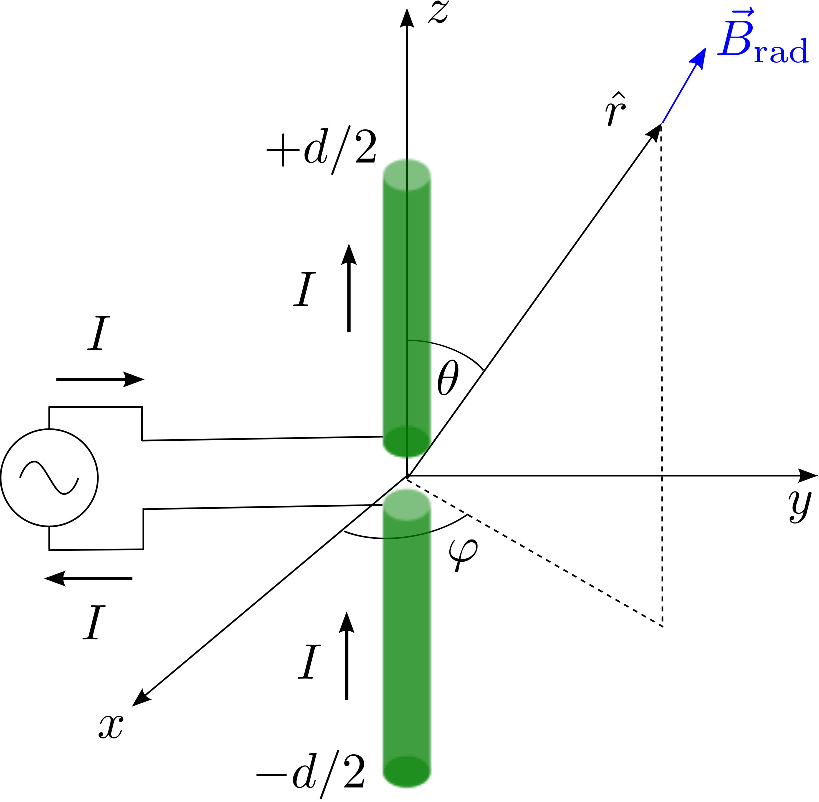
\psfig{file=fig/fig-antena.pdf,width=0.4\textwidth}}
 \caption{Esquema para antena lineal.}
\label{fig:antena}
\end{figure}

Consideraremos el caso en que el largo $d$ de la antena \textit{no} es despreciable comparado con la longitud de onda $\lambda=2\pi c/\omega$ de la radiaci'on emitida. En este caso no es posible utilizar la expansi'on multipolar de la secci'on \ref{sec:emr}. Por lo tanto, para determinar los campos radiativos debemos utilizar la expresiones  (\ref{phirad}) y (\ref{Arad}). En nuestro caso, donde la corriente que circula por el sistema es conocida, basta determinar el potencial vectorial usando (\ref{Arad}), puesto que a partir de 'el podemos calcular el campo magn'etico por medio del rotor. La componente radiativa del campo el'ectrico puede luego determinarse usando $\vec{E}_{\rm rad}=c\vec{B}_{\rm rad}\times\hat{r}$. Adem'as, como en nuestro caso la distribuci'on de corriente es lineal, (\ref{Arad}) se reduce a
\begin{eqnarray}
 \vec{A}_{\rm rad}&=&\frac{\mu}{4\pi}\frac{\hat{z}}{r}\int_{-d/2}^{d/2}I(z,t-\frac{r}{c}+\frac{z}{c}\cos\theta)\,dz \\
&=&\frac{\mu}{4\pi}\frac{\hat{z}I_0}{r}\int_{-d/2}^{d/2}\sen\left(\frac{kd}{2}-k|z|\right)\cos\left[\omega (t-\frac{r}{c}+\frac{z}{c}\cos\theta)\right]\,dz \\
&=&\frac{\mu}{4\pi}\Re\left[\frac{\hat{z}I_0}{r}\int_{-d/2}^{d/2}\sen\left(\frac{kd}{2}-k|z|\right)e^{i\omega (t-\frac{r}{c}+\frac{z}{c}\cos\theta)}\,dz \right]\\
&=&\frac{\mu}{4\pi}\Re\left[\frac{\hat{z}I_0}{r}e^{i\omega(t-\frac{r}{c})}\int_{-d/2}^{d/2}\sen\left(\frac{kd}{2}-k|z|\right)e^{ikz\cos\theta}\,dz \right] .
\end{eqnarray}
La integral involucrada puede ser calculada f'acilmente reduci'endola a integrales de exponenciales, obteniendo:
\begin{equation}
 \int_{-d/2}^{d/2}\sen\left(\frac{kd}{2}-k|z|\right)e^{ikz\cos\theta}\,dz=\frac{2}{k\sen^2\theta}\left[\cos\left(\frac{1}{2}kd\cos\theta\right)-\cos\left(\frac{1}{2}kd\right)\right] .
\end{equation}
Con esto, el potencial vectorial puede escribirse como
\begin{eqnarray}
 \vec{A}_{\rm rad}&=&
\Re\left\lbrace\frac{\mu I_0}{2\pi rk\sen^2\theta}e^{i\omega(t-\frac{r}{c})}\left[\cos\left(\frac{1}{2}kd\cos\theta\right)-\cos\left(\frac{1}{2}kd\right)\right] \right\rbrace\hat{z}\\
&=&\frac{\mu cI_0}{2\pi r\omega}\cos\left[\omega\left(t-\frac{r}{c}\right)\right]\frac{\left[\cos\left(\frac{1}{2}kd\cos\theta\right)-\cos\left(\frac{1}{2}kd\right)\right]}{\sen^2\theta}\hat{z} \\
&=&A_z\hat{z}.
\end{eqnarray}
Determinaremos ahora el campo magn'etico radiativo. Es conveniente calcular el rotor de $\vec{A}$ en coordenadas esf'ericas. Usando $\hat{z}=\hat{r}\cos\theta-\hat{\theta}\sen\theta$
tenemos que $\vec{A}=A_r\hat{r}+A_\theta\hat{\theta}$, con $A_r=A_z\cos\theta$ y $A_\theta=-A_z\sen\theta$. Ya que las componentes de $\vec{A}$ s'olo dependen de $r$ y $\theta$ y que adem'as $A_\varphi=0$ tenemos que el rotor se reduce a
\begin{equation}
 \vec{\nabla}\times\vec{A}=\frac{\hat{\varphi}}{r}\left(\frac{\partial\ }{\partial r}\left(rA_\theta\right)-\frac{\partial A_r}{\partial\theta}\right). \label{rotaa}
\end{equation}
Adem'as, ya que $A_r$ es proporcional a $1/r$, verificamos que el segundo t'ermino de (\ref{rotaa}) aportar'a con un t'ermino proporcional a $1/r^2$ al rotor, que no corresponde a una contribuci'on radiativa al campo magn'etico. De esta forma, llegamos a que
\begin{eqnarray}
 \vec{B}_{\rm rad}&=&\frac{\hat{\varphi}}{r}\frac{\partial\ }{\partial r}\left(rA_\theta\right) \\
&=&-\frac{\hat{\varphi}}{r}\frac{\partial\ }{\partial r}\left(\frac{\mu cI_0}{2\pi\omega}\cos\left[\omega\left(t-\frac{r}{c}\right)\right]\frac{\left[\cos\left(\frac{1}{2}kd\cos\theta\right)-\cos\left(\frac{1}{2}kd\right)\right]}{\sen\theta}\right) \\
&=&-\frac{\mu I_0}{2\pi r}\sen\left[\omega\left(t-\frac{r}{c}\right)\right]\frac{\left[\cos\left(\frac{1}{2}kd\cos\theta\right)-\cos\left(\frac{1}{2}kd\right)\right]}{\sen\theta}\,\hat{\varphi}.
\end{eqnarray}
La potencia instant'anea radiada por unidad de 'angulo s'olido puede entonces calcularse como:
\begin{eqnarray}
 \frac{dP}{d\Omega}&=&\frac{c}{\mu}\left|\vec{B}_{\rm rad}\right|^2 r^2\\
&=&\frac{\mu c I_0^2}{4\pi^2}\sen^2\left[\omega\left(t-\frac{r}{c}\right)\right]\frac{\left[\cos\left(\frac{1}{2}kd\cos\theta\right)-\cos\left(\frac{1}{2}kd\right)\right]^2}{\sen^2\theta}.
\end{eqnarray}
Ya que el movimiento es peri'odico es m'as 'util considerar la potencia promedio radiada:
\begin{equation}
 \left\langle\frac{dP}{d\Omega}\right\rangle=\frac{\mu cI_0^2}{8\pi^2}\left[\frac{\cos\left(\frac{1}{2}kd\cos\theta\right)-\cos\left(\frac{1}{2}kd\right)}{\sen\theta}\right]^2.
\end{equation}
Para una \textit{antena de media onda}, es decir, tal que $d=\lambda/2$, tendremos que $kd=\pi$ y entonces
\begin{equation}
 \left\langle\frac{dP}{d\Omega}\right\rangle=\frac{\mu c I_0^2}{8\pi^2}\frac{\cos^2\left(\frac{\pi}{2}\cos\theta\right)}{\sen^2\theta}.
\end{equation}
%
% Para la antena de una onda $kd=2\pi$:
% \begin{eqnarray}
%  \left\langle\frac{dP}{d\Omega}\right\rangle
% &=&\frac{I_0^2}{2\pi c}\left[\frac{\cos\left(\pi\cos\theta\right)+1}{\sen\theta}\right]^2 \\
% &=&\frac{I_0^2}{2\pi c}\left[\frac{2\cos^2\left(\frac{1}{2}\pi\cos\theta\right)}{\sen\theta}\right]^2 \\
% &=&\frac{2I_0^2}{\pi c}\frac{\cos^4\left(\frac{1}{2}\pi\cos\theta\right)}{\sen^2\theta}
% \end{eqnarray}
\begin{figure}[H]
\centerline{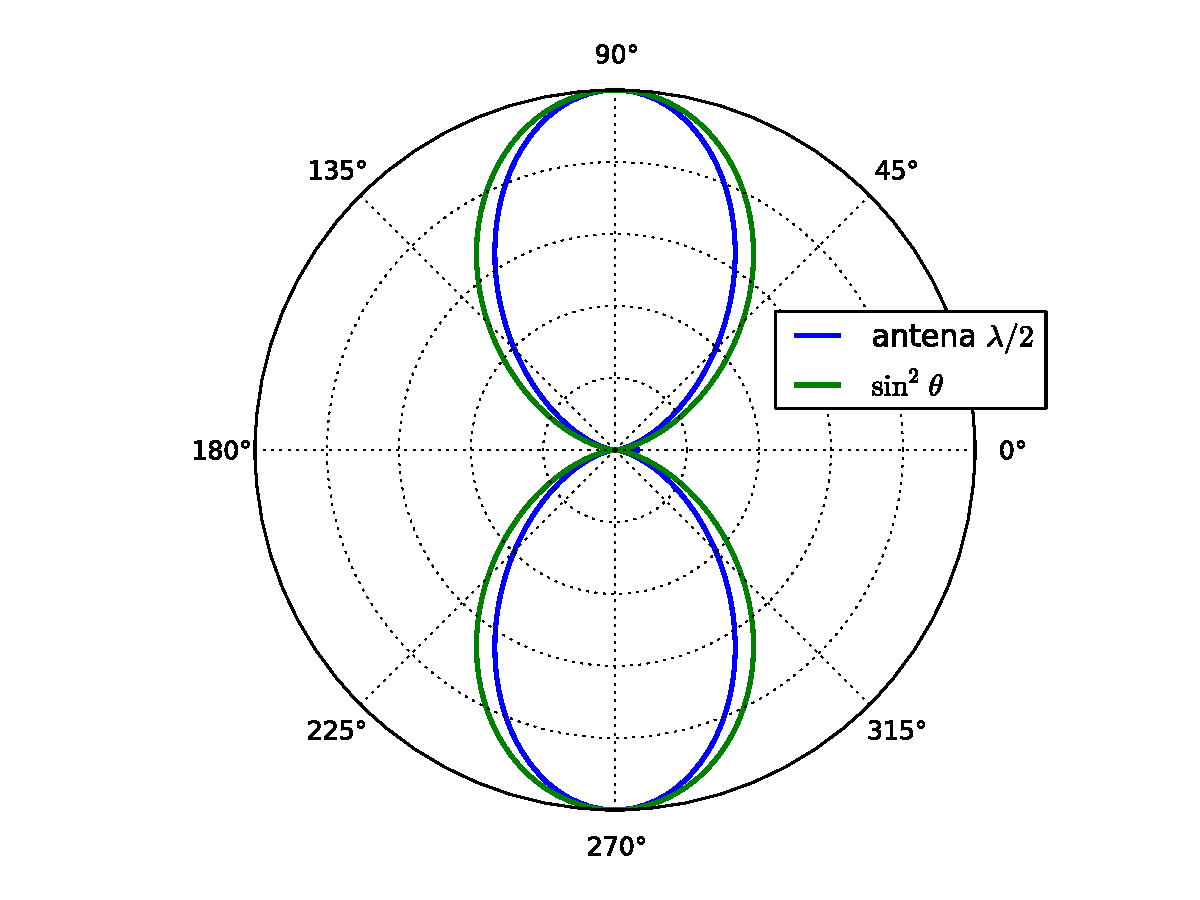
\psfig{file=fig/fig-antena-media-onda.pdf,width=0.5\textwidth}}
 \caption{L\'obulo de radiaci\'on para la antena de media onda en el plano $zx$.}
\label{fig:lobulo_antena}
\end{figure}


En este caso, la potencia promedio total es dada por
\begin{eqnarray}
 \left\langle P\right\rangle
&=&\frac{\mu c I_0^2}{8\pi^2}\int\frac{\cos^2\left(\frac{\pi}{2}\cos\theta\right)}{\sen^2\theta}\,d\Omega \\
&=&\frac{\mu c I_0^2}{4\pi}\int_0^\pi\frac{\cos^2\left(\frac{\pi}{2}\cos\theta\right)}{\sen\theta}\,d\theta\\
&=&\frac{\mu c I_0^2}{4\pi}\times 1.2188\cdots .
\end{eqnarray}
%En unidades S.I., este resultado se expresa como
%\begin{equation}
% \left\langle P\right\rangle
%=\frac{I_0^2}{4\pi\epsilon_0c}\times 1.2188\cdots=\left(\frac{c\mu_0}{4\pi}\times 1.2188\cdots\right)I_0^2.
%\end{equation}
Finalmente evaluando con $c\mu_0/4\pi\approx 30 [NmA^{-2}s^{-1}]$, obtenemos
\begin{equation}
 \left\langle P\right\rangle
=36,564[\Omega]\,I_0^2.
\end{equation}
De aqu'i obtenemos que la \textit{la resistencia de radiaci'on de una antena de media onda} es
\begin{equation}
 R_{\rm rad}\approx 73,13\,\Omega,
\end{equation}
ya que $\left\langle I^2\right\rangle=I_0^2/2$.